%% This document gives an example on how to use the ntnubachelorthesis
%% LaTeX document class.
%% Use oneside for PDF delivery and twoside for printing in a book style
%% use language english, norsk, nynorsk and one of the following shortenings
%%  ``BSP'' Bachelor i Spillprogrammering,\\
%%  ``BRD'' Bachelor i drift av nettverk og datasystemer,\\
%%  ``BIS'' Bachelor i Informasjonssikkerhet,\\
%%  ``BPU'' Bachelor i Programvareutvikling, \\
%%  ``BIND'' Bachelor i Ingeniorfad - data, \\
%%  ``BADR'' Bachelor i drift av datasystemer, \\
%%  ``BIT'' Bachelor i informatikk, \\
%%  ``BABED'' Bachelor i IT-støttet bedriftsutvikling.
%%  ``BMS'' Bachelor i material science.
%%  ``BCE'' Bachelor i chemical science. 
%%  ``BCE'' Bachelor i chemical science.  
%%  ``BPROG''  Bachelor in Programming [Games|Applications]
%%  ``BITSEC''  Bachelor in IT-Operations and Information security 
%%   for example \documentclass[BCE,norsk,twoside]{ntnuthesis/ntnubachelorthesis}

\documentclass[BPROG,english,oneside]{ntnuthesis/ntnubachelorthesis}
%\usepackage[table]{xcolor}
\usepackage[acronym]{glossaries}
\makeglossaries

\usepackage{colortbl}
\usepackage{csvsimple}
\usepackage{booktabs}
\usepackage{parallel,enumitem}
\usepackage{gnuplottex}
\usepackage{pgfplots}\pgfplotsset{compat=1.15}
\usepackage[super]{nth}
\usepackage{soul}
\usepackage{multirow}
\usepackage{graphicx}
\usepackage{float}
\graphicspath{ {inc/images/} }


\usepackage[utf8]{inputenc}
\usepackage[T1]{fontenc}
\usepackage{mathpazo}
\linespread{1.05}
\usepackage{tikz}
\usepackage{dependency/tikz-uml} 
\usepackage[super]{nth}
%\usepackage{amsmath}
%\usepackage{savetrees}

\definecolor{darkgreen}{rgb}{0,0.5,0}
\definecolor{darkred}{rgb}{0.5,0.0,0}

\lstset{ basicstyle=\ttfamily,
                keywordstyle=\color{blue}\ttfamily,
                stringstyle=\color{darkred}\ttfamily,
                commentstyle=\color{darkgreen}\ttfamily,
}


%Typesetting of C++
\newcommand{\CPP}[0]{{C\nolinebreak[4]\hspace{-.1em}\raisebox{.1ex}{\small\bf +\hspace{-.1em}+\ }}}



%\newcommand{\comment}[1]{\textcolor{blue}{\emph{#1}}}  %% use of the colour and you can see how to use commands with parts \comment{so what}

%% The class files defines these two
%% \newcommand{\NTNU}{Norwegian University for Science and Technology} %

% you can create you one #define like structures using the \newcommand feature
% you can change behaviour using \renewcommand

\newcommand{\com}[1]{{\color{red}#1}} % supervisor comment
%\renewcommand{\com}[1]{} %remove starting % to remove supervisor comments
% This will appear in text \com{Lecuters comment} and be visible unless you uncomment
% the renewcommand line.

\newcommand{\todo}[1]{{\color{green}#1}} % items to do
%\renewcommand{\todo}[1]{} %remove starting % to remove items to do

\newcommand{\n}[1]{{\color{blue}#1}} % other comment
%\renewcommand{\n}[1]{} %remove starting % to remove notes

\newcommand{\dn}[1]{} % add the d to a note to say that you have finished with it.

\newcommand{\gj}{NTNU i Gj\o{}vik}

% General purpose commands
\newcommand{\supervisor}{Kolloen, Øivind}
\newcommand{\productowner}{Frantz, Christopher}
\newcommand{\scrummaster}{Torkelsen, Eldar Hauge}
\newcommand{\groupleader}{Holt, Kent Wincent}
\newcommand{\facilitator}{Butt, Zohaib}

% Norwegian Characters,  needs the {} or to be separate from the next letters
% \o{}   \aa{}   \ae{}   so at the end of a word you can use \o  \aa   \ae
% \O{}   \AA{}   \AE{}   you can also just leave a space and latex will remove it
%    eg, NTNU i Gj\o vik  or NTNU i Gj\o{}vik

\begin{document}

\thesistitle{3D Representation of Complex Data Structures}
\thesisshorttitle{Codebase Visualizer 3D} % use this if you have a very long title and want something shorter on the header pages
\thesisauthor{Butt, Zohaib}
\thesisauthorA{Holt, Kent Wincent}
\thesisauthorB{Hauge Torkelsen, Eldar}
%\thesisauthorC{}
\thesissupervisor{\supervisor{}}
%\thesissupervisorA{john smith} %second supervisor


% There use to be a number associated with projects, this would help identify which project was selected.  If you are told to add a project number then this line adds the number.
%\oppgaveNo{29E}

\nmtkeywords{WebGl, Antlr, visualization, programming language, parsing, 3D, Git, MIT}

\nmtdesc{Code-bases can quickly become very large and complex and it's usually difficult to get an overview of the code and it's complexity. We received a task form \productowner{} that would consume a Git repository link and will visualize the code-base that resides within the repository using different colors and shapes. Therefore we've produced a solution that tries to visualize the code in a 3D environment, in a clear and concise way. This resulted in a Web-App containing a back-end API written in Go and an Antlr-based language parser in Java, as well as a front-end written in HTML/CSS/JS. We have tried to follow a professional development method by the use of Scrum, Jira, Confluence as well as high code quality and documentation of both the source code and the development process it-self.}

\nmtoppdragsgiver{\NTNU}
\nmtcontact{\productowner{}}




\thesisdate{\ntnubachelorthesisdate}
\useyear{20.05.2019}

\nmtappnumber{} %number of appendixes
\nmtpagecount{} %currently auto calculated but might be wrong




\thesistitleNOR{3D visualisering av komplekse datastrukturer.}
\nmtkeywordsNOR{WebGl, Antlr, visualisering, programmeringspråk analyse, 3D, Git, MIT}
\nmtdescNOR{Kode-baser kan fort bli store og komplekse, samt kan det ta veldig lang tid å få et overblikk av koden og dens kompleksitet. Vi fikk i oppgave av \productowner{} å implementere et system som kunne ta imot en Git URL og visualisere kode-basen som finnes i Git repositoriet, ved bruk av ulike farger og modeller. Dermed har vi laget en løsning som prøver å visualisere kode i et 3D miljø på en oversiktlig og klar måte. Denne løsningen resulterte til en Web-App med en back-end API i Go og en Antlr-basert språk leser i Java, samt en front-end i HTML/CSS/JS. Vi har prøvd å holde til en professionell utviklings metode, ved bruk av Scrum, Jira og Confluence, samt høy kode kvalitet og dokumentasjon av kildekoden og prosessen.}

 % this is the file which contains all the details about your thesis

\makefrontpages % make the frontpages

\chapter*{Preface} %the * means do not give the chapter a number
\label{chap:preface}

We would like to thank our product owner Frantz, Christopher for making this project and choosing us as the developer team for the project, but also help us improve the product through out bachelor. We would also like to thank our supervisor Kolloen, Øivind for great help in academic writting. A big thanks to participants for user studies and other bachelor students that have helped us correct or shared information related to thesis. We would also like to thank different lecturers and professors that have helped us to gain knowledge which has been used to develop the project and thanks to McCallum, Simon for making the \LaTeX{} template which was used to write the thesis.
 
 


\tableofcontents
\listoffigures
\listoftables
\lstlistoflistings
\printglossaries

% Language definitions
\lstset{ 
  backgroundcolor=\color{white},   % choose the background color; you must add \usepackage{color} or \usepackage{xcolor}; should come as last argument
  basicstyle=\footnotesize,        % the size of the fonts that are used for the code
  breakatwhitespace=false,         % sets if automatic breaks should only happen at whitespace
  breaklines=true,                 % sets automatic line breaking
  captionpos=b,                    % sets the caption-position to bottom
  %commentstyle=\color{mygreen},    % comment style
  deletekeywords={...},            % if you want to delete keywords from the given language
  escapeinside={\%*}{*)},          % if you want to add LaTeX within your code
  extendedchars=true,              % lets you use non-ASCII characters; for 8-bits encodings only, does not work with UTF-8
  firstnumber=0,                    % start line enumeration with line 1000
  %frame=single,	                   % adds a frame around the code
  keepspaces=true,                 % keeps spaces in text, useful for keeping indentation of code (possibly needs columns=flexible)
  keywordstyle=\color{blue},       % keyword style
  language=Octave,                 % the language of the code
  morekeywords={*,...},            % if you want to add more keywords to the set
  numbers=left,                    % where to put the line-numbers; possible values are (none, left, right)
  numbersep=5pt,                   % how far the line-numbers are from the code
  %numberstyle=\tiny\color{mygray}, % the style that is used for the line-numbers
  rulecolor=\color{black},         % if not set, the frame-color may be changed on line-breaks within not-black text (e.g. comments (green here))
  showspaces=false,                % show spaces everywhere adding particular underscores; it overrides 'showstringspaces'
  showstringspaces=false,          % underline spaces within strings only
  showtabs=false,                  % show tabs within strings adding particular underscores
  stepnumber=1,                    % the step between two line-numbers. If it's 1, each line will be numbered
  %stringstyle=\color{mymauve},     % string literal style
  tabsize=2,	                   % sets default tabsize to 2 spaces
  title=\lstname                   % show the filename of files included with \lstinputlisting; also try caption instead of title
  literate={å}{{\a}}1
            {ø}{{\o}}1
            {æ}{{\ae}}1
}

% Taken from Lena Herrmann at 
% http://lenaherrmann.net/2010/05/20/javascript-syntax-highlighting-in-the-latex-listings-package

\lstdefinelanguage{JavaScript}{
  keywords={typeof, new, true, false, catch, function, return, null, catch, switch, var, if, in, while, do, else, case, break},
keywordstyle=\color{teal}\bfseries,
  ndkeywords={class, export, boolean, throw, implements, import, this},
  ndkeywordstyle=\color{darkgray}\bfseries,
  identifierstyle=\color{black},
  sensitive=false,
  comment=[l]{//},
  morecomment=[s]{/*}{*/},
  commentstyle=\color{purple}\ttfamily,
  stringstyle=\color{brown}\ttfamily,
  morestring=[b]',
  morestring=[b]"
}

% Taken from Lena Herrmann at 
% http://lenaherrmann.net/2010/05/20/javascript-syntax-highlighting-in-the-latex-listings-package

\lstdefinelanguage{AntlrGrammar}{
    keywords={grammar, fragment},
    keywordstyle=\color{teal}\bfseries,
    ndkeywords={grammar, fragment},
    ndkeywordstyle=\color{darkgray}\bfseries,
    identifierstyle=\color{blue},
    sensitive=false,
    comment=[l]{//},
    morecomment=[s]{/*}{*/},
    commentstyle=\color{purple}\ttfamily,
    stringstyle=\color{brown}\ttfamily,
    morestring=[b]',
    morestring=[b]"
}

% From https://github.com/COPCSE-NTNU/bachelor-thesis-NTNU/blob/master/inc/implementation.tex
\lstdefinelanguage{go}
    {   morekeywords={var, for, int, string , float, struct, func, package, import},
        sensitive=false,
        morecomment=[l]{//},
        morecomment=[s]{/*}{*/},
        morestring=[b]",
        basicstyle=\ttfamily,
        keywordstyle=\color{teal}\bfseries,
        stringstyle=\color{brown}\bfseries,
        commentstyle=\color{purple}\bfseries
}


\chapter{Introduction}
\label{chap:introduction}

\section{Background}
% Should we introduce the state of the world before or after presenting the product owner? 
\newglossaryentry{whitebox}{name={white-box}, description={Software testing approaches that examine the program structure and derive test data from the program logic \cite{enc:whitebox}}}
\newglossaryentry{controlFlow}{name={Control flow}, description={The order of which a programs instructions or statements are executed \cite{wiki:controlFlow}}}
This project was requested by \productowner{} from the Department of Computer Science at \NTNUgjovik. The project was requested because finding libraries or frameworks that would fit well for new software projects can be a time consuming and difficult process that might require \gls{whitebox} analysis. This project should make the \gls{whitebox} analysis easier by abstracting the code and representing it as a 3D graphical structure and giving information on complexity and quality of the project. 

CodePark \cite{DBLP:journals/corr/abs-1708-02174} and CodeCity \cite{wettel2010software} are two applications trying to solve the same type of problem with similar 3D solution, representing the code as houses or city blocks. CodePark visualize the code-base in park-like environment. Each class in the code-base is represented as a interactable cube. In the cube, all functions in each class are visible on the wall and upon a click, it highlights the function in the code, which is shown on a separate wall. CodeCity represents the code as navigable cities, where each building represents a class and each district represents a package.

The two examples differ from this project in how this project will represent connections related to \gls{controlFlow} and the code not being represented as buildings or cities. This project will also represent different data-structures such as vectors and maps.

\section{Subject area}

Our software is meant to be used in a software development setting. Software development \cite{wiki:softwareDevelopment} includes many different processes such as system specification, software reuse, integration, development, testing and maintenance. Our system will mostly help with the software reuse and integration part, but will also indirectly affect the other processes.

System specification deals with identifying what the system should do and the environment it acts in.

Software reuse takes those specifications and identifies preexisting systems that could be used instead of developing new software. This process often identifies libraries and frameworks that can be used, which is often recommended \cite{Krueger:1992:SR:130844.130856} in both large and small systems. Developers spend a lot of time debugging, securing, documenting, structuring or finding suitable libraries and frameworks, etc. This can be frustrating and time consuming if there is no good documentation, source code or life cycle provided \cite{mileva2009mining}.

Software integration takes the preexisting systems or the software it integrates with and molds them to fit smoothly. The integration can vary in difficulty depending on the implementation of each software solution. 

Software development creates the functionality that is not provided by preexisting solutions. It is recommended to have as little code complexity \cite{DBLP:journals/corr/abs-1712-00675} as possible for readability  \cite{spinellis2003readingWritingCode} which can be hard for developers to see while programming and is partially reliant on how well the software integration went. Potential problems with the preexisting systems are likely to emerge at this state as it is difficult to see limitation and bugs during the software integration phase. Finding bugs in this scenario is time-consuming \cite{westland2002cost} and might require the developers to do white-box testing on an unfamiliar system.
Bugs that are not found during development will hopefully be found during software testing.

Software testing validates that the functionality works as expected with no side-effects. This can help spot bugs or shortcomings in the preexisting systems. If bugs are not found during software testing, then they are likely to persist through the life cycle of the software or until identified by the user

Software maintenance deals with updating the software to remove issues found by users or through normal use. It also assures that dependencies stay up to date.

The problem our system will help with is giving an impression of the build and quality of libraries and frameworks that are considered by the software reuse process. The system will act as a lesser alternative to documentation or as a quick overview to the libraries or framework.

\section{Boundaries}
\newglossaryentry{qualitymetric}{name={quality metric}, description={A rule for quantifying some characteristic or attribute of a computer software entity.
One of a set of techniques whose aim is to measure the quality of a computer program. \cite{enc:softwaremetric}}}
The system is not meant to help with software specification or the later stages of development after software integration. It is not meant to supersede or be an exhaustive substitution of documentation, but rather an abstraction and quick overview of the code base. The abstraction will be limited to a 3D visualization and textual representation of metric and meta data. It will not change the software in question or improve the quality, but give the end user an insight into the software model and code quality. 
The project will not involve developing new \glspl{qualitymetric}, but use preexisting metrics that have been used by other developers and been proven to be help-full.

The system will not build, nor execute the code-base in question but rather do static analysis. There will neither be provided any test coverage nor execution of any shipped testing functionality.

\section{Target group}
Target groups for the project can be divided into two parts; Application users and thesis readers.

\subsection{Web Application Users}
\newacronym{it}{IT}{Information Technology}
The web application mainly targets three different settings or context;
\begin{itemize}
    \item Academic - Students, lecturer or researchers studying \gls{it}. 
    \item Professional - \gls{it} developers.
    \item Amateur - hobbyists looking into \gls{it}.
\end{itemize}

\subsubsection{Academic}
\newglossaryentry{oop}{name={object-oriented programming}, description={Object-oriented programming is a programming paradigm based on the concept of "objects", which can contain data, and code, in the form of procedures}}
In an academic setting, the application can be used by students to check for code quality and complexity of their hand-in or their work. However the students must be familiar to concept like \gls{oop} to understand the visual output from the system. These students are expected to have at least one programming related semester for the system to be useful. 

Lecturers can use the system in the lectures to explain the differences between loosely and highly coupled architectures or discuss code quality.

\subsubsection{Professional and amateur}
The main target groups of this web-application are programmers in both professional and amateur settings. Here the application will be used mainly by the lead programmer as well as developers and architects to decide whether a library or framework should be used in production by assessing its complexity. 

Programmers that are in the learning phase might find this application useful because of its 3D visualization of the code-base which will help them to see the whole code-base as one structured and clear representation.

\subsection{Thesis readers}
\newglossaryentry{opensource}{name={open-source}, description={Open source is a term denoting that a product includes permission to use its source code, design documents, or content \cite{wiki:opensource}}}
Target group for the thesis is anyone interested in knowing about the development process, motivation or implementation of the project. First and foremost anyone involved in the grading process, but also any developer who would take the project further as an \gls{opensource} project or other derived work.
This thesis is a natural followup after reading the documentation provided in the \gls{git} repository.

\section{Motivation}
\newglossaryentry{devops}{name=DevOps, description={A set of practices that aim to improve connections between development and operations and shorten the development liefecycle while ensuring high quality}}
%
% REFACTORING: Continue refactoring from here
%
The project description shown in appendix \ref{appendix:initialProjectDescription}, indicated great potential and was interesting . It allowed for flexibility and depth, by spanning a variety of technologies and subject areas. It mentioned web-technologies, language parsing, complex data-structures, visualization with interaction and container technologies. For the group it was a good mix of familiar technologies for exploration and unfamiliar concepts to study. The project would allow for a practical application of \gls{devops} and system architecture which the group had a more theoretical understanding of. It would also explore language parsing that the group has a very limited knowledge of and associate with low-level, complicated or compiler related subject areas. Parsing would allow for a deep dive into niche aspects of C++, Java or other programming languages. In addition the project was about static analysis that could help to improve understanding of code quality. The main motivation was the high learning outcome.

\subsection{Background competence}
\label{sec:competence}

The groups knowledge that was considered relevant for the project included:
%%
%% How should be reference the course descriptions?
%%
\begin{itemize}
    \item Operating systems - All members had theoretical knowledge through a course and practical experience with Linux as main driver for several years.
    \item Architecture and static analysis - All members had a theoretical understanding through the software engineering and software security course but lacked more in depth practical experience.
    \item Visualization and interaction - All members had experience through the graphics programming and the games programming courses. 
    \item Complex data-structures - All members had theoretical experience through math for programming, math for computer science and algorithmic methods.
    \item Web-development - All members had experience through Cloud Technologies course. Besides, individual members had experience through Web Technology course, software security project or learning assistant task. 
\end{itemize}
\subsection{Competence to acquire}
\begin{itemize}
    \item Static analysis
    \item Language parsing
    \item Quality metrics and measures
    \item Complex data representation
    \item Client-side technologies  
\end{itemize}

\section{Constraints}

\subsubsection{Legal Constraints}
\begin{itemize}
%%%%%
% Product owner:
%   Add references.
%%%%%
    \item The resulting system will not be in violation of general data protection regulation. \cite{lovdata:gdpr}
    %\item ISO/IEC 27000 in regards to security.
    \item The system will not be in violation of Norwegian copyright act.
\end{itemize}

\subsubsection{Technological Constraints}

\begin{itemize}
    \item The system should be cross platform.
    \item The system should be dockerized.
    \item The system should have a REST API.
    \item The resulting system will not be in violation of general data protection regulation. \cite{lovdata:gdpr}
    %\item ISO/IEC 27000 in regards to security.
    \item The system will not be in violation of Norwegian copyright act.
\end{itemize}

\subsection{Time Constraints}
Project planning started \nth{5} Jan 2019.

\begin{itemize}
    \item The system should be finalized by \nth{16} May.
\end{itemize}

\section{Roles}
\subsection{Group roles}
\newglossaryentry{leadProg}{name=Lead programmer, description={The person who's responsible for ensuring good code efficiency and quality}}
\newglossaryentry{releaseMgr}{name=Release Manager, description={The person who's responsible for releasing production ready software}}
\newglossaryentry{devOpsEvang}{name=DevOps evangelist, description={The person who researches and pushes for DevOps concepts and methodologies}}
\newglossaryentry{scrumMaster}{name=Scrum Master, description={The person that manages sprints, backlog.}}
\newglossaryentry{automationArchitect}{name=Automation Architect, description={The person who's responsible for, design, implementation and analyzation of strategies for continuous deployments whilst ensuring high availability of product and pre-production stages}}
\newglossaryentry{leadSecurityEngineer}{name=Lead Security Engineer, description={The person who gives recommendations towards security and enforces them as much as possible}}
\newglossaryentry{recorder}{name=Recorder, description={The person who produces reports from meetings}}
\newglossaryentry{leadInteractionDesigner}{name=Lead Interaction Designer, description={The person who's responsible for ensuring that interactions are user-friendly}}
\newglossaryentry{XAProf}{name=Experience Assurance Professional, description={The person who's responsible for ensuring focus on user experience in any new and old functionality}}
\newglossaryentry{facilitator}{name=Facilitator, description={The person who readies materials for meetings}}
\newglossaryentry{utilityTechnologyPlayer}{name=Utility Technology Player, description={The person who's responsible of maintaining uptime of service and give inputs on security, quality and resource management}}

\begin{table}[H]
\centering
\begin{tabular}{|l|l|}
\hline
\multicolumn{2}{|c|}{ \cellcolor[HTML]{AFAFAF} Group roles} \\
\hline
    \cellcolor[HTML]{AFAFAF} Member & \cellcolor[HTML]{AFAFAF} Role \\
\hline
\multirow{4}{*}{Kent Wincent Holt - 473209} 
 & The Group leader \\
 & \gls{leadProg} \\
 & Software developer/tester \\
 & \gls{releaseMgr} \\

\hline
\multirow{5}{*}{Eldar Hauge Torkelsen - 473180} 
 & \gls{devOpsEvang} \\
 & \gls{scrumMaster} \\
 & \gls{automationArchitect} \\ 
 & Software developer/tester \\
 & \gls{leadSecurityEngineer} \\
 & \gls{recorder} \\
 & \gls{leadInteractionDesigner} \\
 
\hline
\multirow{4}{*}{Zohaib Butt - 473219 } 
 & Software developer/tester \\
 & \gls{XAProf} \\
 & \gls{facilitator} \\
 & \gls{utilityTechnologyPlayer} \\
\hline
\end{tabular}
\caption{Group roles}
\end{table}

\subsection{Other roles}
The other roles involved in the thesis are supervisor and product owner.
\begin{itemize}
    \item The supervisor role is filled by \supervisor{} and will be responsible for providing the feedback, insights and corrections on both report structure and content.
    \item The product owner role is filled by \productowner{} and will be responsible for providing wanted criteria. Discussing these criteria regarding how time consuming and how demanding they are. Upcoming planned sprint will also be discussed with product owner.
\end{itemize}

\newacronym{imrad}{IMRaD}{Introduction, Material and method, Results and Discussion}

\section{About Report}
The report contains a lot of acronyms and expressions as these are commonly used in a development setting, but they might not be intuitive and therefor a glossary has been included to solve this problem. The structure of the report is based on \gls{imrad}-model and provided template for bachelor thesis by \NTNUgjovik{}.


\chapter{Requirements}
\label{chap:requirements}

The group have divided the requirements in three sections: result goals, operational requirements and learning outcomes. Result goals defines what the group expect to deliver as the end product. Operational requirements describe what the team expect from the system after a set amount of time and are listed to give an indication of the intended quality of the final system. Learning outcomes describe what the team wants to learn during development and thesis writing.

\section{Result Goal}
    \begin{itemize}
        \item Program must, at a minimum, be able to abstract and visualize language version up to Java 11.0.2 and C++17.
        \item Code visualization must be in 3D.
        \item Program must give an indication of the quality of the software code.  
        \item Program must be able to take a link to a git repository to use as basis for visualization.
        \item Program must be able to show potential execution paths or program flow through the program.
        \item Program must have a public facing API for developers.
        \item Program must be dockerized. 
        \item The user must be able to interact with the 3D visualization to show implementation of data structures.
        \item The system must present complexity metrics to the user.
        \item The system must give an indication on where complexity arises.
    \end{itemize}
    
\section{Operational requirements}
\newacronym{vcpu}{VCPU}{Virtual Central Processing Unit}
\newacronym{gb}{GB}{GigaByte}
\newacronym{kloc}{KLOC}{Thousands of Lines Of Code}
    The following operational requirements assumes a server equivalent of a \gls{skyhigh} instance of flavor c1.tiny with 16 \gls{gb} of ram, 40 \gls{gb} of disk space and 8 \glspl{vcpu}.  
    \begin{enumerate}  
        \item Quantitative goals for the system: 
        \begin{itemize}
            \item The system must handle 30 concurrent users with repository of less than 10 \gls{kloc} while using less than 10 minutes of processing time.
            \item The system must be able to handle a peak of at least 60 users.
            \item The system must be able to handle repositories of less than 100 \gls{kloc}. 
        \end{itemize}
        \item Qualitative goals for the system:
        \begin{itemize}
            \item The system must help developer(s) gain overview and an understanding of the code base.
            \item The system must let the user easily navigate through the visualization.
            \item The system must be naturally intuitive and easy-to-use for new users.
            \item The system must be accessible to people with minor disabilities, like colorblindness. 
        \end{itemize}
    \end{enumerate}
        
\section{Learning outcome}
    \begin{itemize}
        \item Learn in depths \gls{webgl} technology.
        \item Learn professionalism in web development.
        \item Understand and follow \gls{devops} methodology throughout the project.
        \item Learn in depths dockerizing containers.
        \item Learn \gls{frontend} web frameworks.
        \item Learn about different code quality metrics for static analysis.
        \item Learn about professional web architectures.
        \item Learn about \gls{iac}.
    \end{itemize}

\section{Use Case}
\newglossaryentry{usecase}{name=use case, description={Usually a list of events, often used to describe the interaction between actors and systems}}

To achieve more detailed view of the actual systems functionality that need to be implemented, it is important to visualize the system from users perspective without focusing on implementation details. To do this, \glspl{usecase} and a use-case diagram are used as they show users needs.



\begin{figure}[H]
\begin{tikzpicture}
\begin{umlsystem}{System}
\umlusecase[x=-2, y=0, name=highlightConn]{Highlight connection between data-structures}
\umlusecase[x=0, y=1, name=submitRepo]{Submit git repository}
\umlusecase[x=0, y=8.5, name=loadRepo]{Load other repository stored in DB}
\umlusecase[x=2, y=2, name=navigate]{Navigation of visualization}
\umlusecase[x=0, y=4, name=getImpl]{Get implementation of data-structure}
\umlusecase[x=0, y=5, name=qualityMet]{Select quality metrics} 
\umlusecase[x=0, y=6, name=lexer]{Adding a lexer file}
\umlusecase[x=2, y=3, name=color-scheme]{Add a custom color-scheme}
\umlusecase[x=0, y=7, name=GUI]{Change GUI layout}
\umlusecase[x=-3, y=10, name=codebase]{Get representation of codebase}
\end{umlsystem}

\umlactor[x=-9, y=4]{User}


\umlassoc{User}{highlightConn}
\umlassoc{User}{submitRepo}
\umlassoc{User}{loadRepo}
\umlassoc{User}{navigate}
\umlassoc{User}{getImpl}
\umlassoc{User}{qualityMet}
\umlassoc{User}{lexer}
\umlassoc{User}{color-scheme}
\umlassoc{User}{GUI}
\umlassoc{User}{codebase}

\umlinclude{codebase}{loadRepo}

\end{tikzpicture}
\caption{Use case diagram.}
\end{figure}


\subsection{High level use case descriptions}
\noindent\fbox{
    \parbox{\textwidth}{
        \textbf{Use case name:} Change GUI layout                                  \\
        \textbf{Actors:} User                                                        \\
        \textbf{Target:} Target is to change the GUI layout in the application.       \\
        \textbf{Description:} User can change the GUI layout by dragging and scaling windows. User can also add or remove a window of same type or any other type.   
    }
} \\ \\

\noindent\fbox{
    \parbox{\textwidth}{
        \textbf{Use case name:} Add a color-scheme                                 \\
        \textbf{Actors:} User                                                        \\
        \textbf{Target:} Target is to change the color-scheme used in the application. \\
        \textbf{Description:} User can change the color-scheme of application by specifying a set of colors from a palette on the home page.   
    }
} \\ \\


\noindent\fbox{
    \parbox{\textwidth}{
        \textbf{Use case name:} Add a lexer file                                  \\
        \textbf{Actors:} User                                                      \\
        \textbf{Target:} User can add new lexer file to the system.         \\
        \textbf{Description:} User can submit a new lexer files on the home page by clicking on the "upload lexer file" and choosing the file from a remote machine.
    }
} \\ \\

\noindent\fbox{
    \parbox{\textwidth}{
        \textbf{Use case name:} Select quality metrics                              \\
        \textbf{Actors:} User                                                       \\
        \textbf{Target:} User can select a specific quality metric.         \\
        \textbf{Description:} User can choose between different quality metrics such as "connascence measure", "cyclomatic complexity" and "Halstead complexity measures" on the quality metrics window. The chosen metrics will then be used for analysis of the submitted codebase.
    }
} \\ \\

\noindent\fbox{
    \parbox{\textwidth}{
        \textbf{Use case name:} Submit git repository                               \\
        \textbf{Actors:} User                                                         \\
        \textbf{Target:} User can submit the git repository               \\
        \textbf{Description:} User can submit the git repository by adding repository link on the text field with name "Git Repository" and click submit to store repository in the database. The field can be found at home page.
    }
} \\ \\

\noindent\fbox{
    \parbox{\textwidth}{
        \textbf{Use case name:} Load other repository stored in DB                   \\
        \textbf{Actors:} User                                                         \\
        \textbf{Target:} User can load the repositories submitted by other users.     \\
        \textbf{Description:} Database has multiple repositories stored by different users. These repositories will be shown in the window named "Repositories". A user can click on available repositories to visualize it.
    }
} \\ \\

\noindent\fbox{
    \parbox{\textwidth}{
        \textbf{Use case name:} Get implementation of data structure                   \\
        \textbf{Actors:} User                                                         \\
        \textbf{Target:} User can see the implementation of chosen data structure.    \\
        \textbf{Description:} This functionality is required to have at least one entry in the database so that the system can get the representation of codebase. Once the visualization of codebase is shown, user can choose between visualized data structures to see the implementation on a window named "Implementation".
    }
} \\ \\

\noindent\fbox{
    \parbox{\textwidth}{
        \textbf{Use case name:} Navigation of visualization                   \\
        \textbf{Actors:} User                                                         \\
        \textbf{Target:} User can navigate in the 3D environment to see visualized models. \\
        \textbf{Description:} This functionality requires a submitted repository so that the representation of codebase can be shown. The navigation includes rotation, translation and zoom. The user can navigate in 3D environment using mouse or keyboard.
    }
} \\ \\

\noindent\fbox{
    \parbox{\textwidth}{
        \textbf{Use case name:} Highlight connection between data structure          \\
        \textbf{Actors:} User                                                         \\
        \textbf{Target:} Highlighting relations between data structures. \\
        \textbf{Description:} This functionality requires a submitted repository so that the representation of codebase can be shown. Once the codebase is visualized, the user can choose between different data structures visualized to highlight it's links with other data structures. Highlighting connections will brighten the color of all the links and connected data structures, but also dull the color of all the unconnected data structures.
    }
} \\ \\

\noindent\fbox{
    \parbox{\textwidth}{
        \textbf{Use case name:} Get representation of codebase       \\
        \textbf{Actors:} User             \\
        \textbf{Target:} Visualizing the codebase in 3D environment.  \\
        \textbf{Description:} The user starts at the homepage where the git repository to be visualize needs to be submitted. Once the requested git link is submitted and stored in database, user is taken to loading page where user can see the status of processing codebase file from back-end server. After the processing is done user is taken to 3D visualization page where the visualization will show the different data structures represented as a shape and a color. 
    }
} \\ \\
\section{Product backlog}
\begin{table}
    \resizebox{\columnwidth}{!}{
        \csvautotabular{inc/csv/finalIssuelist.csv}
    }
    \caption{Final backlog}
    \label{finalBacklog}
    
\end{table}
The final backlog can be seen in table \ref{finalBacklog}. It show a more detailed view than what is described in the use cases. 

\section{Domain model}
\begin{figure}[H]
\begin{tikzpicture}

\umlemptyclass[x=0, y=-3]{User}
\umlemptyclass[x=0, y=-6]{Visualization}
\umlclass[x=0, y=-10]{Quality metrics}{
    name : str\\
    value[] : int\\
    quality rank : str\\
}{}

\umlclass[x=5, y=-3]{Git Project}{
    URI : str \\
    commitLog[] : str
}{}
\umlemptyclass[x=5, y=-6]{Project Code}

\umlclass[x=10, y=-6]{Source File}{
    language : str \\
    content : str 
}{}
\umlclass[x=10, y=-12]{Language Parser}{
    language : str 
}{}

\umlclass[x=6.5, y=-8]{Syntax Rule}{
     syntax: str \\
}{}

\umlclass[x=5, y=-12]{Code Structure}{
    name : str\\
}{}

\umlemptyclass[x=0.5, y=-15]{Namespace}
\umlemptyclass[x=3, y=-15]{Class}
\umlclass[x=5, y=-15]{Function}{
}{}
\umlclass[x=7, y=-15]{Variable}{
    value : str\\
    name : str\\
    type : str\\
}{}
\umlemptyclass[x=9, y=-15]{Template}
\umlemptyclass[x=11, y=-15]{Call}

\umlclass[x=7, y=-18]{Argument}{
}{}

\umlassoc[geometry=-|, arg1=1..1, anchor2=-180, arg2=1..*] 
    {User}{Git Project}
\umlassoc[geometry=-|,  arg1=1..1, anchor2=-180, arg2=1..1 ]
    {Visualization}{Project Code}
\umlassoc[geometry=-|-, arg1=1..*, pos1=1, anchor2=-160, arg2=1..1, pos2=2.5]
    {Quality metrics}{Project Code}

\umlassoc[arg1=1..1, pos1=0.05, anchor2=-90, arg2=1..1, pos2=0.65] 
    {Source File}{Language Parser}
\umlassoc[geometry=-|, arg1=1..1, pos1=1.55, anchor2=90, arg2=1..1, pos2=1.9] 
    {Git Project}{Project Code}
\umlassoc[geometry=-|, arg1=1..1, pos1=0.1, anchor2=90, arg2=1..*, pos2=0.55] 
    {Project Code}{Source File}

\umluniassoc[arg1=0..*, angle1=10, angle2=50, loopsize=1.5cm]
    {Syntax Rule}{Syntax Rule}
    
\umlNarynode[x=6.5,y=-10, name=languageStructureSyntax, below]{}
    \umlassoc[arg1=0..*]{Syntax Rule}{languageStructureSyntax}  
    \umlassoc[geometry=|-, anchor1=120, arg1=1..1]{Language Parser}{languageStructureSyntax}  
    \umlassoc[geometry=|-, arg1=0..*]{Code Structure}{languageStructureSyntax} 

\umluniassoc[arg1=0..*, angle1=10, angle2=50, loopsize=1.5cm]
    {Code Structure}{Code Structure}


\umlinherit[geometry=|-|]{Namespace}{Code Structure}
\umlinherit[geometry=|-|]{Class}    {Code Structure}
\umlinherit[geometry=|-|]{Function} {Code Structure}
\umlinherit[geometry=|-|]{Variable} {Code Structure}
\umlinherit[geometry=|-|]{Template} {Code Structure}
\umlinherit[geometry=|-|]{Call}     {Code Structure}

\umlcompo[]{Variable}{Argument}
\umlassoc[geometry=-|, arg1=0..*, arg2=0..1, pos2=1.8]{Argument}{Call} 


\end{tikzpicture}
\caption{Domain model.}
\label{fig:domainModel}
\end{figure}

\newglossaryentry{recursion}{name=recursion, description={A computer programming technique involving the use of a procedure, subroutine, function, or algorithm that calls itself one or more times until a specified condition is met at which time the rest of each repetition is processed from the last one called to the first }}
\newglossaryentry{recursive}{name=recursive, description={Of, relating to, or involving \gls{recursion}}}
\newglossaryentry{syntax}{name=syntax, description={The way in which linguistic elements (such as words) are put together to form constituents (such as phrases or clauses)}}

Figure \ref{fig:domainModel} shows a crude overview of the subject area relating to the project. The code structure is language dependent and \gls{recursive} based on the \gls{syntax} rules relating to the structure. The relationship between a call, variable and parameter relates to how a function-call can have parameters that define which overloaded version of a function is being called. This relationship is given as an example but there are many other similar relationships that have not been added for clarity, like how variable types such as classes can define the scope a function is being called from. This is a relationship between functions being defined as part of a class, variables being instances of said class and calls being called on said variable.

\Gls{syntax} rules are also \gls{recursive} as they can be defined by a set of rules or a character sequence.

\section{Risk assessment}
The initial task description and product owner did not give any specific security requirements and has therefore done a risk assessment to identify any shortcomings that might happen and how to deal with them. This risk assessment will be a part of the base for the security requirements.

\subsection{Identification and project risk analysis}
\newglossaryentry{manhattanDistance}{name={manhattan distance}, description={The distance between two points measured along axes at right angles \cite{manhattanDistance}}}
The table \ref{riskOverview} contains possible risks based on \cite{DBLP:journals/corr/abs-1708-02174} and compared with the system requirements. The probabilities and effects are estimates done by the core team. The priority is based on the minimal \gls{manhattanDistance} from top right corner of table \ref{riskForm}.

c\begin{table}[H]
\centering
\resizebox{\columnwidth}{!}{
 \begin{tabular}{| c | c | l | c | c | c |} 
 \hline
 \cellcolor[HTML]{AFAFAF} Id & \cellcolor[HTML]{AFAFAF} Risk Type & \cellcolor[HTML]{AFAFAF} \cellcolor[HTML]{AFAFAF} Possible Risk & \cellcolor[HTML]{AFAFAF} Priority & \cellcolor[HTML]{AFAFAF} Probability & \cellcolor[HTML]{AFAFAF} Effect                     \\  
 \hline\hline
 1 & Organization & Losing important data & 7 & Low & Significant                           \\ 
 \hline
 2 & Technology & Technology components aren't scalable & 4 & Medium & Severe              \\
 \hline
 3 & Technology & Sanitation of input from external sources & 10 & Medium & Significant    \\
 \hline
 4 & Technology & Application instability & 5 & Low & Severe                                           \\
 \hline
 5 & Organization & Team members are unavailable for longer period of time & 6 & Medium & Significant            \\
 \hline
 6 & Requirement & Discovering problems in requirements at delivery & 1 & High & Severe     \\
 \hline
 7 & Estimate & Project size is under estimated & 3 & High & Significant                    \\
 \hline
 8 & Organization & Learning curves lead to delays & 2 & Very High & Moderate \\
 \hline
 9 & Technology & Integration testing environments aren't available & 9 & Low & Minor       \\
 \hline
 10 & Organization & Fail to follow software methodology & 8 & Medium & Minimal             \\
 \hline
 11 & Technology & Exposure of sensitive personal or corporate data & 11 & Very Low & Severe             \\
 \hline
 12 & Technology & Incapability of identifying individual or corporate entity & 12 & Very Low & Moderate             \\
 \hline
 13 & Technology & Illegal use of stored software & 13 & Low & Significant             \\
 \hline
\end{tabular}
}
\caption{Overview of risks}
\label{riskOverview}
\end{table}

\begin{table}[H]
    \centering
        \begin{tabular}{| c | c | c | c | c | c |} 
            \hline
            \cellcolor[HTML]{AFAFAF} & Minimal & Minor & 
                                       Moderate & Significant & 
                                       Severe    \\  
            \hline\hline
            Very High  &    \cellcolor[HTML]{FFEA00} & \cellcolor[HTML]{FFEA00} & 
                            \cellcolor[HTML]{FF0004} 8 & \cellcolor[HTML]{FF0004} &
                            \cellcolor[HTML]{FF0004}  \\ 
            \hline
            High       &    \cellcolor[HTML]{FFEA00} & \cellcolor[HTML]{FFEA00} & 
                            \cellcolor[HTML]{FFEA00} & \cellcolor[HTML]{FF0004} 7 & 
                            \cellcolor[HTML]{FF0004} 6 \\
            \hline
            Medium     &    \cellcolor[HTML]{00FF1D} 10& \cellcolor[HTML]{FFEA00} & 
                            \cellcolor[HTML]{FFEA00} & \cellcolor[HTML]{FFEA00} 3, 5 &
                            \cellcolor[HTML]{FF0004} 2 \\
            \hline
            Low        &    \cellcolor[HTML]{00FF1D} & \cellcolor[HTML]{00FF1D} 9 & 
                            \cellcolor[HTML]{FFEA00} & \cellcolor[HTML]{FFEA00} 1, 13 & 
                            \cellcolor[HTML]{FFEA00} 4 \\
            \hline
            Very Low   &    \cellcolor[HTML]{00FF1D} & \cellcolor[HTML]{00FF1D} & 
                            \cellcolor[HTML]{00FF1D} 12 & \cellcolor[HTML]{FFEA00} & 
                            \cellcolor[HTML]{FFEA00} 11 \\ [1ex]
            \hline
        \end{tabular}
    \caption{Risk analysis form}
    \label{riskForm}
\end{table}

\subsection{Risk mitigation strategy}

Table \ref{riskMitigation} shows the mitigation strategy for the project risks with highest priority and should give an overview of mitigations that should help with most of the identified risks, as several can be mitigated with similar strategies.

% 4 & Technology & Application instability & 5 & Low & Severe
% 5 & Organization & Team members are unavailable for longer period of time & 6 & Medium & Significant
% 1 & Organization & Losing important data & 7 & Low & Significant
% 10 & Organization & Fail to follow software methodology & 8 & Medium & Minimal
% 9 & Technology & Integration testing environments aren't available & 9 & Low & Minor
% 3 & Technology & Sanitation of input from external sources & 10 & Medium & Significant
% 11 & Technology & Exposure of sensitive personal or corporate data & 11 & Very Low & Severe
% 12 & Technology & Incapability of identifying individual or corporate entity & 12 & Very Low & Moderate
% 13 & Technology & Illegal use of stored software & 13 & Low & Significant
\begin{table}[H]
\resizebox{\columnwidth}{!}{
\begin{tabular}{|c|l|p{10cm}|}
    \hline
    \cellcolor[HTML]{AFAFAF} Priority & \cellcolor[HTML]{AFAFAF} Risk & \cellcolor[HTML]{AFAFAF} Mitigation  \\
    \hline
    \hline
    1 & Discovering problems in requirements at delivery
    & \begin{itemize}
        \item Use an agile development process 
        \item Perform regular user testing
    \end{itemize} \\ 
    \hline
    2 & Learning curve lead to delay 
    & \begin{itemize}
        \item When a new technology is to be used, a workshop for exploring it will be held
    \end{itemize}\\
    \hline
    3 & Project size is under estimate
    & \begin{itemize}
        \item Use an agile development process
        \item Have regular meetings with product owner 
    \end{itemize} \\
    \hline
        4 & Technology components are not scalable
        & \begin{itemize}
            \item Use IaC and code for modularity 
        \end{itemize}\\
    \hline
    5 & Application instability
    &\begin{itemize}
        \item Unit test coverage of all important functions
        \item Use DevOps with live server throughout the development
    \end{itemize} \\
    \hline
    6 & Team members are unavailable for longer period of time
    &\begin{itemize}
        \item Focus on reviewing git pull requests well
        \item Good communication amongst developers
    \end{itemize}\\
    \hline
    7 & Losing important data
    &\begin{itemize}
        \item Use cloud storage
        \item Additional data storage security systems
        \item Have and take regular backups
    \end{itemize}\\
    \hline
    
\end{tabular}
}
\caption{Risk mitigation}
\label{riskMitigation}
\end{table}

\newglossaryentry{git}{name=Git, description={Version control system}}
\newglossaryentry{dosAttack}{name=DOS-attack, description={Denial of Service attack}}
\newglossaryentry{proprietary}{name=proprietary, description={Closed source}}
\newglossaryentry{xssAttack}{name=XSS-attack, description={Cross site scripting, input executable code that will run on other instances of the service}}
\newglossaryentry{sql}{name=SQL, description={Structured Query Language used for Querying from certain database systems}}
\newglossaryentry{sqliAttack}{name=SQLi-attack, description={\gls{sql} injection, input of executable \gls{sql} code that could modify a \gls{sql}-based database system}}

\section{Security requirements}
\begin{itemize}
    \item Sanitization of input from external sources within visualization and field for repository link submission to mitigate \gls{sqliAttack} and \gls{xssAttack}s.
    \item The application will not in any way record or process any data that can be used to identify usage patterns for individual or corporation. 
    \item Application will not store nor expose sensitive personal or corporate project information.
    \item The submitted repositories that are stored, are only stored for visualization of the codebase and will not at any point be built by the application.
    \item Any submitted repository will not be used for any other purpose than for visualization and quality assessment.
    \item Extensive testing to mitigate instabilities.
\end{itemize}
\chapter{Technical Design}
\label{chap:technical}

\section{Architecture}

\begin{figure}[h] 
    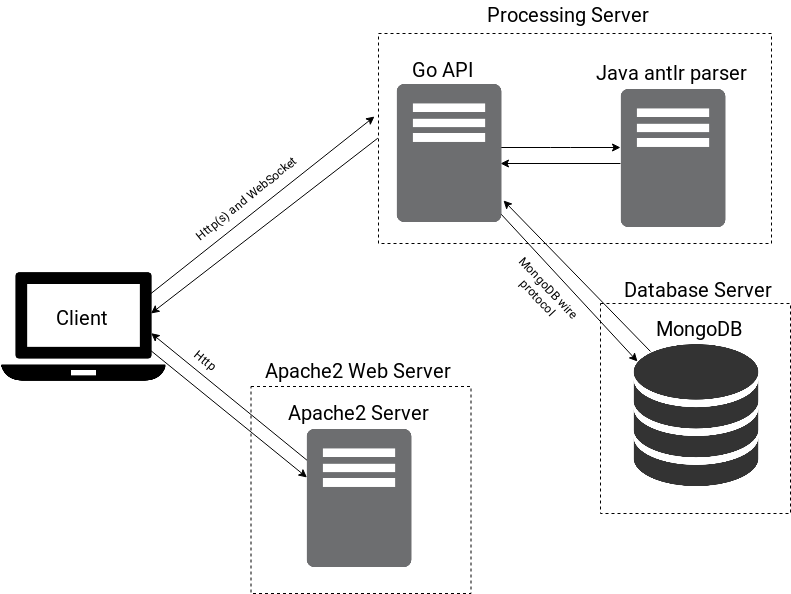
\includegraphics[width=\textwidth]{inc/images/CoVi_Architecture.png}
    \caption{System architecture.}
    \label{fig:architecture}
\end{figure}

\newacronym{api}{API}{Application Programming \Gls{interface}}
\newacronym{html}{HTML}{Hyper Text Markup Language}
\newacronym{css}{CSS}{Cascading Style Sheets}
\newacronym{http}{HTTP}{Hypertext Transfer Protocol}
\newacronym{antlr}{ANTLR}{ANother Tool for Language Recognition}
\newacronym{mvc}{MVC}{Model View Controller}
\newglossaryentry{server}{name=server, description={Computer in a network that is used to provide services  to other computers in the network}}
\newglossaryentry{client}{name=client, description={Computer in a network that uses the services provided by a \gls{server}}}
\newglossaryentry{js}{name=JavaScript, description={A "call by sharing" scripting language often used for \gls{client}-side web-applications}}
\newglossaryentry{websocket}{name=WebSocket, description={WebSockets is communication protocol, providing three communication channals; "Open", "Close", "Message" over a single transmission control protocol connection}}
\newglossaryentry{backend}{name=back-end, description={Back-end is the data access layer of a software}}
\newglossaryentry{Antlr}{name=Antlr, description={\gls{antlr} is a powerful parser generator for reading, processing, executing, or translating structured text or binary files. \cite{parr2013definitive}}}

As the figure \ref{fig:architecture} shows, the team divided the different components of the system. Initially the team had planned to implement the solution as a modern REST-full \gls{api}, where \gls{client} sends request to processing server for data to be handled. \Gls{client} uses \gls{http} and \glspl{websocket} to communicate with go \gls{api}, the reason \glspl{websocket} are used is because of lacking update on status of back-end processing for \gls{client} side.\glspl{websocket} can send multiple responses to the one sending request, this way we were able to show the status of processing to the \gls{client}.

Processing server consist of two components Go \gls{api} and Java antlr parser. Go \gls{api} is a REST-full \gls{api} but with some functionality implemented as \glspl{websocket}. Go \gls{api} is the common interface that \gls{client} communicate to store or receive data from the database server.Java \gls{antlr} parser is stand-alone helper application used by go \gls{api} to parse submitted project files. During implementation of the Java \gls{antlr} Parser, the team did some research to find the best way to use \gls{antlr} for parsing project files. Apache2 web server is used to send the \gls{html}, \gls{css} and \gls{js} to the \gls{client} through \gls{http} protocol. Database server is used by Go \gls{api} to update and fetch the data based upon \glspl{client} request.

\subsection{Front-end}
\newglossaryentry{interface}{name=interface, description={The means by which interaction or communication is achieved between systems}}
\newacronym{ui}{UI}{User \Gls{interface}}
\newglossaryentry{apache2}{name=apache2, description={A free and open-source cross-platform web server \cite{apacheServer}}}
\newglossaryentry{golang}{name=golang, description={Golang or Go is a statically typed compiled language in the tradition of C, with memory safety, garbage collection, structural typing, and CSP-style concurrent programming features added}}
\newacronym{fdg}{FDG}{Force Directed Graph}
\newacronym{loc}{LOC}{Lines Of Code}
\newacronym{json}{JSON}{\gls{js} Object Notation}
\newglossaryentry{namespace}{name=namespace,description={A named scope that prevents symbols from being mistaken for identically-named symbols in other scopes}}

\begin{figure}
\noindent\rule{\textwidth}{1pt}
\begin{lstlisting}[language=JavaScript, caption= {JSON structure from api}, label={lst:apiFormat}]
{
  "statuscode": 200,
  "statustext": "OK",
  "body":{
     "fileCount": 0,
     "id": "5cc9c475b7fa706ccb4700f1",
     "parsedFileCount": 0,
     "result": {
       "files": [
         {
           "parsed": false,
           "file_name": "5cc9c475b7fa706ccb4700f1/README.md",
           "linesInFile": 0
         },
         {
           "parsed": true,
           "file_name": "5cc9c475b7fa706ccb4700f1/main.cpp",
           "functions": [
             {
               "name": "main()",
               "declrator_id": "main",
               "return_type": "int",
               "function_body": {
                 "calls": [
                   {
                     "identifier": "printHelloWorld()",
                     "scopes": [
                       {
                         "identifier": "World",
                         "type": "namespace"
                       }
                     ]
                   }
                 ]
               },
               "start_line": 15,
               "end_line": 19
             }
           ],
           "namespaces": [],
           "linesInFile": 18
         }
       ]
     },
     "skippedFileCount": 0,
     "status": "Done"
  }
}
\end{lstlisting}
\noindent\rule{\textwidth}{1pt}
\end{figure}

The \gls{ui} form is given from a static \gls{apache2} server and populated by a dynamic \Gls{golang} server. The front-end consists of two separate parts; project info and code-base visualization.

The code-base visualization is where the functionality lies. It communicate with the \gls{api} to acquire a language independent representation of the code-base and getting parts of the code-base source. It expects the \gls{api} to serve \gls{json} in a similar format to listing \ref{lst:apiFormat}. The different parts of the response can be explained as below:
\begin{itemize}
    \item statuscode and statustext - Refers to a \gls{http} status to create a more uniform interface with \glspl{websocket} and normal \gls{http} requests.
    \item body - The requested data with what is required to represent the code-base and information on the completeness of the parsing.
    \item files - Represents a sourcefile in the repository
    \item functions, namespaces, classes, variable - Code blocks that the \gls{client} expect to contain code blocks for visualization
    \item call - A function call or assignment found in function code-block.
    \item scope - Shows if a call is executed on a variable.
\end{itemize}

Although what type of code-block can be within a type of code-block might depend on the language, the \gls{client} application allows for any code-block within any other and relies on the structure from the \gls{api} to be correct. This is done to make the application as language independent as possible.

The \gls{api} result is parsed to create the visualization with scopes, identifiers and relations. The representation is structured using a \gls{fdg} to space out separate structures with related structures close together and unrelated structures further apart. Each scope goes through the \gls{fdg} separately so to ensure that the scope is maintained in the representation whilst the scopes internal relations are based on the calls. The calls are connected to closest structure found to the function being called. The call might not always be connected to the actual function as the called function might be outside the repository or can not be identified due to the parser limitations. 

In addition the code-base visualization has a textual description of project metadata such as \gls{loc} and number of structures like \glspl{namespace}, classes and functions, that were found.

The project info part describes the project, refers to the \gls{git} repository  and describes the limitations of the program.

The limitations include unsupported browsers and limitations created by the incomplete parsing or unhandled code constructs.

\subsection{Back-end}
\label{sec:technicalBackEnd}
The processing server is the main server in \gls{backend}. It is responsible for handling the request from \gls{client} and send a response with a meaningful \gls{http} status code. Java \gls{Antlr} parser within the processing server is a stand-alone java application that uses \gls{Antlr} for language processing. \gls{Antlr} is a language recognition tool that uses a grammar file to assign a lexer token to each rule and then matches the token with a character sequence in the parsed file. \gls{Antlr} provides a listener for each rule in the grammar file. Once a rule matches a lexer token, it will callback to the respective listener. With this setup it became very straight forward to use \gls{Antlr} but it took a lot of time to understand the grammar files. Grammar files are created by different contributors which means names given for rules in the grammar are dependent on the contributor's choice and made it very hard for us to find rules for very specific language functionalities.

Go \gls{api} uses parts of \gls{mvc} pattern. \gls{mvc} pattern is widely used within web development because it excludes the coupling between \gls{ui} and logic. Go \gls{api} uses the model and controller parts of \gls{mvc} and view is managed by \gls{frontend}. Controller in go \gls{api} is responsible of handling validation, error handling and business logic whilst models represents abstraction of data model and encapsulates database handling.

Java \gls{Antlr} parser is designed to take in two arguments; file path and target language used in the file. In return Java \gls{Antlr} parser will output the parsed code in \gls{json} format to the standard output channel. The \gls{json} format was necessary so that parsed code would be uniformed for both C++ and Java targets. The parser takes only one file at a time so that Go \gls{api} could filter the project files that system does not support. This helped in limiting the \gls{Antlr} processing time.

As figure \ref{fig:sequenceInitial} shows, Go \gls{api} is responsible for handling requests from \gls{client}, validation, execution of Java \gls{Antlr} parser and handling database. For the initial request from user, Go \gls{api} will first check the database if project has been parsed previously and return the cached parsed code-base. If no caching has been done Go \gls{api} executes the Java \gls{Antlr} parser and passes the file to be parsed along with a target based on file's extension.

If the project to be parsed has multiple files Go \gls{api} will check what files of the project are supported by the Java \gls{Antlr} parser and will only send those files as an argument one at a time. Once the parser output is received in Go \gls{api}, it will construct and add the output  into project \gls{json}. Once all supported files are parsed, the project \gls{json} will be sent as a response to \gls{client}.

% talk about mvc and sequence diagram of initial request.
\begin{figure}[H] 
    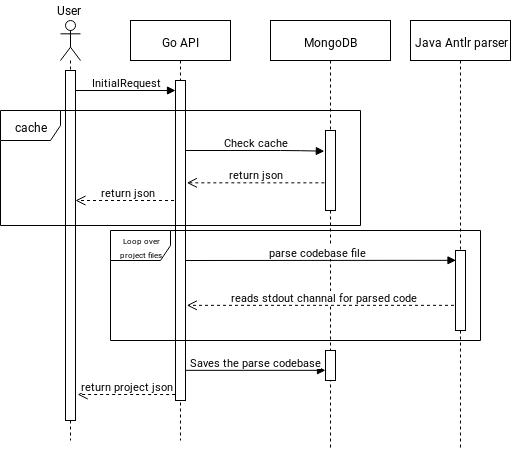
\includegraphics[width=\textwidth]{inc/images/InitialRequestSequenceDiagram.png}
    \caption{Sequence diagram of Initial request.}
    \label{fig:sequenceInitial}
\end{figure}

\subsection{WEB API}
\newacronym{uid}{UID}{Unique IDentifier}
% DRAFT!!!

At the start there was a requirement to have a REST-based \gls{api} to receive information about a given project. We therefore came up with the following structure:
\begin{itemize}
    \item /repo/add - Addition of a repository to the servers, this will, if it doesn't exist, clone it and return a new \gls{uid} else it returns the existing \gls{uid}.
    \item /repo/list - List all repositories that has been added to the server. So the user can see what's been parsed before.
    \item /repo/\{repoId\}/initial/ - The initial request used to fetch project structure and complexity measures. In the beginning this was a \gls{http}-method and since parsing a repository takes a long time, it could result in the user getting annoyed that no feedback on progress is returned. It was decided then that the initial \gls{api} endpoint would be upgraded to a web-socket that can maintain a connection and send multiple packets more naturally than basic \gls{http}-methods. This made us drift form the requirement of full a REST-based \gls{api} but to re-fulfill this requirement we could re-implement the original endpoint and serve it together with the web-socket.  
    
    The final result of the parsing is also cached for a quicker response, but the caching mechanics is every crude in the sense that it doesn't update the cached data even if the submitted repository has changed.
    \item /repo/\{repoId\}/file/read/ - Used to fetch any implementation at a specified location and size, in a given file.
\end{itemize}

A lot of focus was put on documentation, the group decided therefore to use \gls{api} Doc for this purpose. The generated documentation is hosted using an \Gls{apache2} web server. 
\chapter{User Interface}
\label{chap:UI}

\section{Design}

\begin{figure}[h]
    \centering
    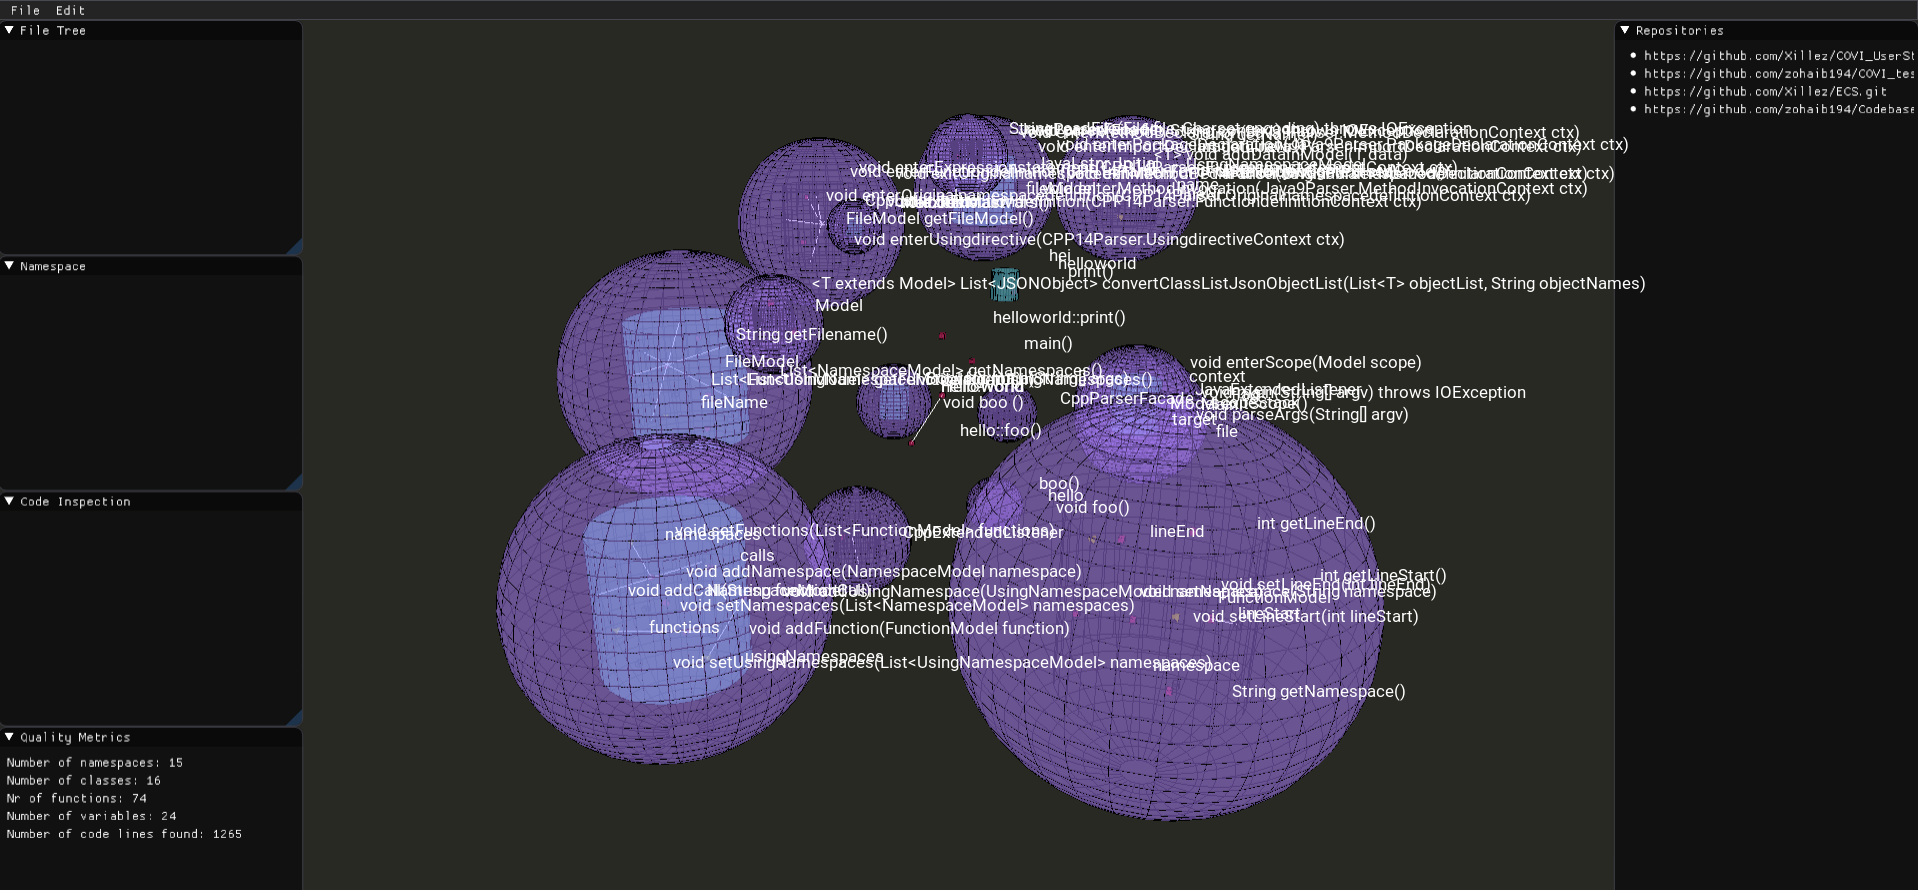
\includegraphics[width=\textwidth]{inc/images/COVI_Visualization.png}
    \caption{Final UI layout.}
    \label{fig:finalui}
\end{figure}
\newglossaryentry{tensorflow}{name={Tensorflow}, description={An end-to-end open source platform for machine learning \cite{tensorflow}}}

The initial \gls{ui} concept shown in appendix \ref{app:initialConcept}, was presented to product owner during the second meeting to visualize how the team had intended to design layout of the system. Product owner was pleased by the looks of the system and approved it.

\gls{tensorflow} visualization was an inspiration because it deals with concepts like AI and big data, which have quite understandable and readable ways to represent a big data set through graphs. The team wanted an intuitive way of visualizing the data structure along with keeping the concepts like loosely or highly coupled relationships. Therefore the \gls{tensorflow} representation seemed a perfect fit for this problem.

The left side of figure \ref{app:initialConcept}, was meant to show project related data such as file structure, namespaces, implementation and quality metrics. Whilst the right side shows project independent data, such as repositories registered in the system for easy switching between them. 

The final \gls{ui} layout is shown in figure \ref{fig:finalui}.
\chapter{Development process}
\label{chap:process}

\section{Development methodology}
\newglossaryentry{developmentMethodology}{name={development methodology}, description={A framework that is used to structure, plan, and control the process of developing an information system}}

When considering \gls{developmentMethodology} it was important to choose one that would fit the project and fit the prioritizations of both the product owner and the development team.
The teams project independent priorities were:
\begin{itemize}
    \item High focus on code
    \item Embedded documentation
    \item Self documenting code
    \item A good fit for teams experience level
    \item Ability to tackles miss-estimation
    \item Team focus
\end{itemize}

Product owner gave the impression that professionalism, high code quality and an independent development team was important.

\section{Choice of methodology}
\label{sec:methodology}
Apart from the project independent priorities mentioned in the previous section, the team considered these project features as leading when choosing \gls{developmentMethodology}:

\begin{itemize}
    \item Ambiguous specification - A general desire was given, but details were left to the development team.
    \item Research focus - Project differed greatly from other projects.
    \item Likely to change over time
    \item Require additional knowledge - The team had limited to no knowledge on some topics as mentioned in section \ref{sec:competence}
\end{itemize}
\newglossaryentry{agile}{name=agile, description={\Gls{developmentMethodology} focused on adaptability and requirements or solutions to evolve through the collaborative effort of self-organizing and cross-functional teams and their end user. \cite{beck2001manifesto}}}
\newglossaryentry{scrum}{name=Scrum, description={A framework within which people can address complex adaptive problems, while productively and creatively delivering products of the highest possible value. \cite{schwaberScrum.2017}}}

The team had to plan for high degree of uncertainty, making \gls{agile} a requirement. With the teams experience level, it seemed like \gls{scrum} would be a good fit. \Gls{scrum} fits well with the focus on code and code-quality, but would still generate enough documentation to help with professionalism. 
The team used ideas from \gls{devops} along with \gls{scrum}, to improve documentation and embed the documentation together with the code.  

\section{Execution}
\newglossaryentry{sprint}{name=sprint, description={A time constrained unit of work in \gls{scrum}}}
\newglossaryentry{formatter}{name=formatter, description={A computer program used for formatting}}
\newglossaryentry{vetter}{name=vetter, description={A computer program used for formatting source code}}
\newglossaryentry{linter}{name=linter, description={A tool that analyzes source code to flag programming errors, bugs, stylistic errors, and suspicious constructs}}
\newglossaryentry{documentationGenerator}{name={documentation generator}, description={A programming tool that generates software documentation from a set of source code files}}
\newglossaryentry{apidoc}{name={APIDOC}, description={Generates a RESTful web API Documentation \cite{github:apidoc}}}
\newglossaryentry{godoc}{name={Godoc}, description={Extracts and generates documentation for Go programs}}
\newglossaryentry{jsdoc}{name={JSDoc}, description={Markup language used to annotate JavaScript source code files}}
\newglossaryentry{docker}{name={Docker}, description={A computer program that performs operating-system-level virtualization known as containerization}}
\newglossaryentry{dockerfile}{name={dockerfile}, description={File containing instructions for automating \gls{docker} container setup}}
\newglossaryentry{dockercompose}{name={Docker Compose}, description={A tool for defining and running multi-container \gls{docker} applications}}
\newacronym{iac}{IaC}{Infrastructure as Code}
\newglossaryentry{fullstack}{name={full-stack}, description={Anything that touches all levels between \gls{client} and \gls{backend}}}
\newglossaryentry{jira}{name={Jira}, description={A proprietary issue tracking product}}
\newglossaryentry{confluence}{name={Confluence}, description={A collaboration software program developed and published by Atlassian}}

The team worked with one week long \glspl{sprint}, starting on Tuesday morning and finishing on Monday evening. The \gls{sprint} length meant that underestimated tasks would not cause too large of a disruption and the team could quickly change priorities. One \gls{sprint} lasted for two weeks as the quantity of work was large and provided little opportunity for change in priorities. 

All member worked in the same room during a significant majority of the time, with high levels of communication. Each member worked with their own tasks taken from the backlog, and requested help if needed.

When a task was submitted, it would be reviewed by both other members and accepted or had changes requested. While reviewing, the team members would often discuss in person with the one who submitted, to assure that both had the same interpretation of the solution. The requirements for a submission to be accepted was quite high, often rejected due to spelling errors or lacking comments. Before a submission it was also required to run \gls{formatter}, \gls{vetter} and \gls{linter} in addition to documenting through comments following the relevant \gls{documentationGenerator}: \gls{apidoc}, \gls{godoc} or \gls{jsdoc}. Initially the idea was to also do documentation trough \gls{iac}, but due to the continual underestimation of tasks, it was not followed up on. \Glspl{dockerfile} and \gls{dockercompose} are still present and working, but were outdated for a large portion of the development.

\begin{figure}[H]
    \noindent\rule{\textwidth}{1pt}    
    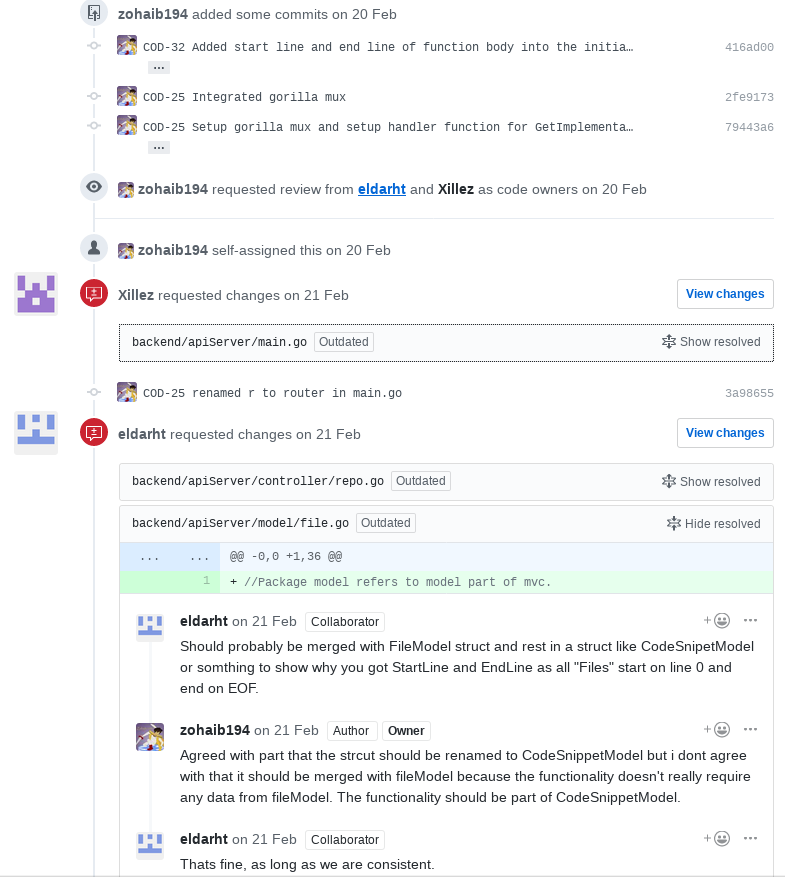
\includegraphics[width=\textwidth]{inc/images/pullrequestDiscussion.png}
    \noindent\rule{\textwidth}{1pt}
    \caption{Pull request discussion.}
    \label{fig:pullrequestDiscussion}
\end{figure}

Project status was documented with \gls{jira}, \gls{confluence} and \gls{git}.

Mondays were used for meetings and started off by having a meeting with supervisor followed by preparation for meeting with product owner, then said meeting and ended with retrospective meeting or internal meetings.

\subsubsection{Meetings with supervisor}
\newglossaryentry{reviewMeeting}{name={review meeting}, description={A process where \gls{scrum} team shows what was accomplished during the \gls{sprint} \cite{schwaberScrum.2017}}}
Meetings with supervisor were used as a \gls{sprint} \gls{reviewMeeting}, discussing what was completed or not in the last \gls{sprint}, and how the team worked. Suggestions on how to improve the development process or documentation and professionalism were given to the team.  

\subsubsection{Meetings with product owner}

\newglossaryentry{backlog}{name={product backlog}, description={An ordered list of everything that is known to be needed in the product \cite{schwaberScrum.2017}}}
\newglossaryentry{sprintbacklog}{name={sprint backlog}, description={Set of \gls{backlog} items selected for the \gls{sprint} \cite{schwaberScrum.2017}}}
\newglossaryentry{softwaredesignpattern}{name={software design pattern}, description={A reusable solution to a commonly occurring problem within a given context in software design}}
\newglossaryentry{planningMeeting}{name={planning meeting}, description={A process where product owner describes highest priority feature to the team}}

Planning for the meeting with product owner consisted of preparing a suggestion for a \gls{sprintbacklog}. The meetings were used as \gls{sprint} \gls{reviewMeeting} and \gls{sprint} \gls{planningMeeting}. General recommendations were given as well as specific recommendations on choice of technology or \gls{softwaredesignpattern}. The suggested \gls{sprintbacklog} was looked over and finalized according to product owner's input. 

\subsubsection{Internal meetings}
\newglossaryentry{sprintretrospective}{name={sprint retrospective}, description={Meeting for planning improvements to be enacted during the next \gls{sprint} \cite{schwaberScrum.2017}}}
Internal meetings were used for \gls{sprintretrospective} meetings and for story point estimation of the upcoming \gls{sprint}. 

\subsubsection{Story points}
\newglossaryentry{storypoint}{name={story point}, description={ An abstract measure of effort required to implement a user story}}

\begin{figure}[H]
    \noindent\rule{\textwidth}{1pt}    
    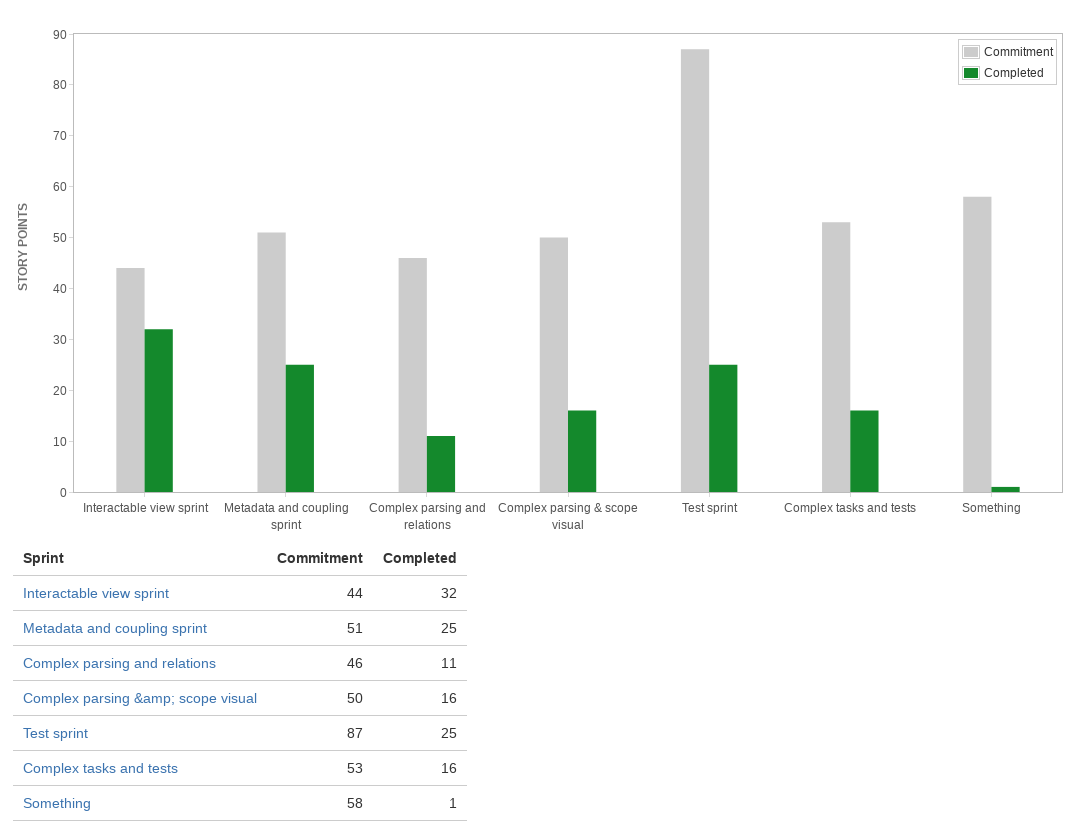
\includegraphics[width=\textwidth]{inc/images/velocity.png}
    \noindent\rule{\textwidth}{1pt}
    \caption{Velocity chart.}
    \label{fig:velocityChart}
\end{figure}

For estimation \glspl{storypoint} were used. \Glspl{storypoint} were given based on relative size, and time value changed over time. This change meant that the teams velocity as shown in figure \ref{fig:velocityChart} is misleading.

\subsubsection{Scrum board}
\begin{figure}[H]
    \noindent\rule{\textwidth}{1pt}    
    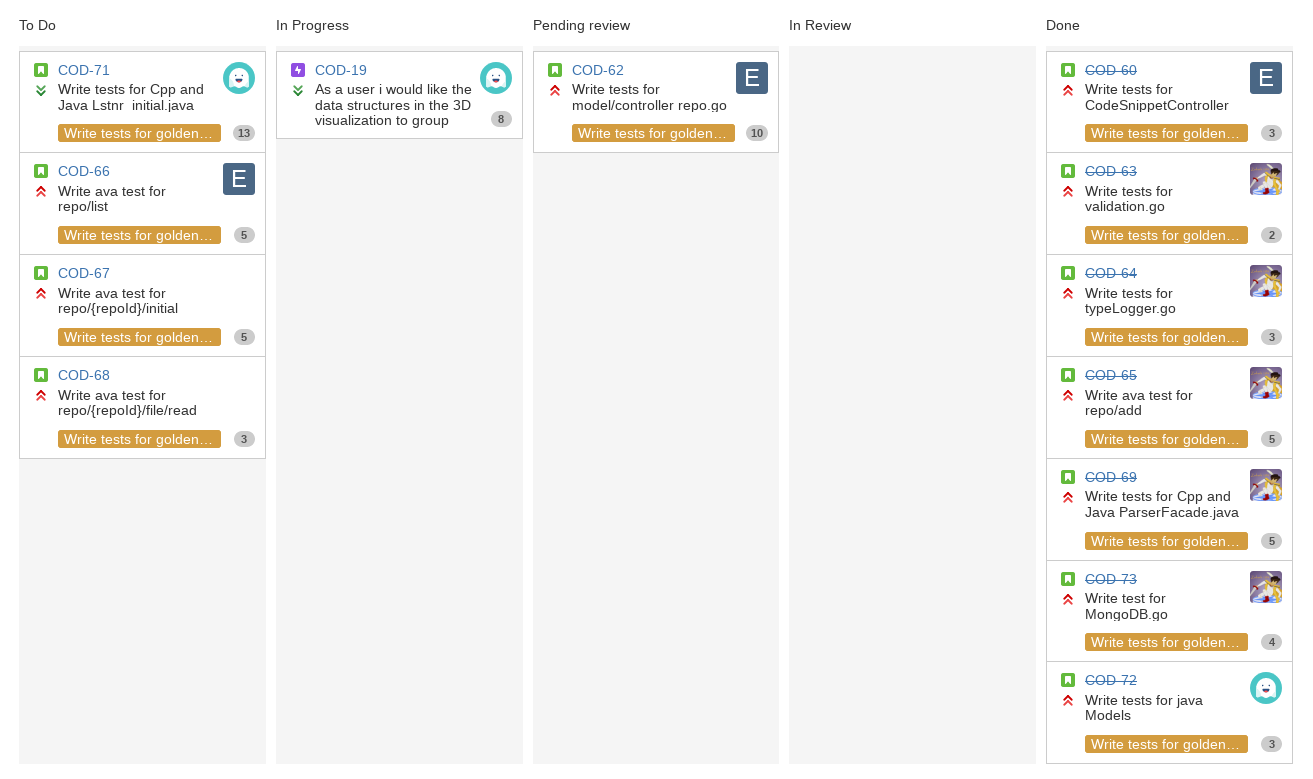
\includegraphics[width=\textwidth]{inc/images/board.png}
    \noindent\rule{\textwidth}{1pt}
    \caption{Scrum board for test sprint.}
    \label{fig:scrumBoar}
\end{figure}

As shown in figure \ref{fig:scrumBoar}, the workflow was divided into five parts:

\begin{itemize}
    \item "To Do" - \Gls{sprintbacklog}.
    \item "In Progress" - Tasks currently being worked on.
    \item "Pending review" - Developer consider the task completed and want other team members to review it.
    \item "In Review" - Team member has reviewed task and requested changes.
    \item "Done" - Team members have accepted and merged pull request.
\end{itemize}

\section{Sprint Overview}
\newglossaryentry{burndown}{name={burndown}, description={A graphical representation of work left to do versus time \cite{wiki:burndown}}}
\subsection{Sprint: hello world (02. feb - 13. feb)}
\begin{figure}[H] 
    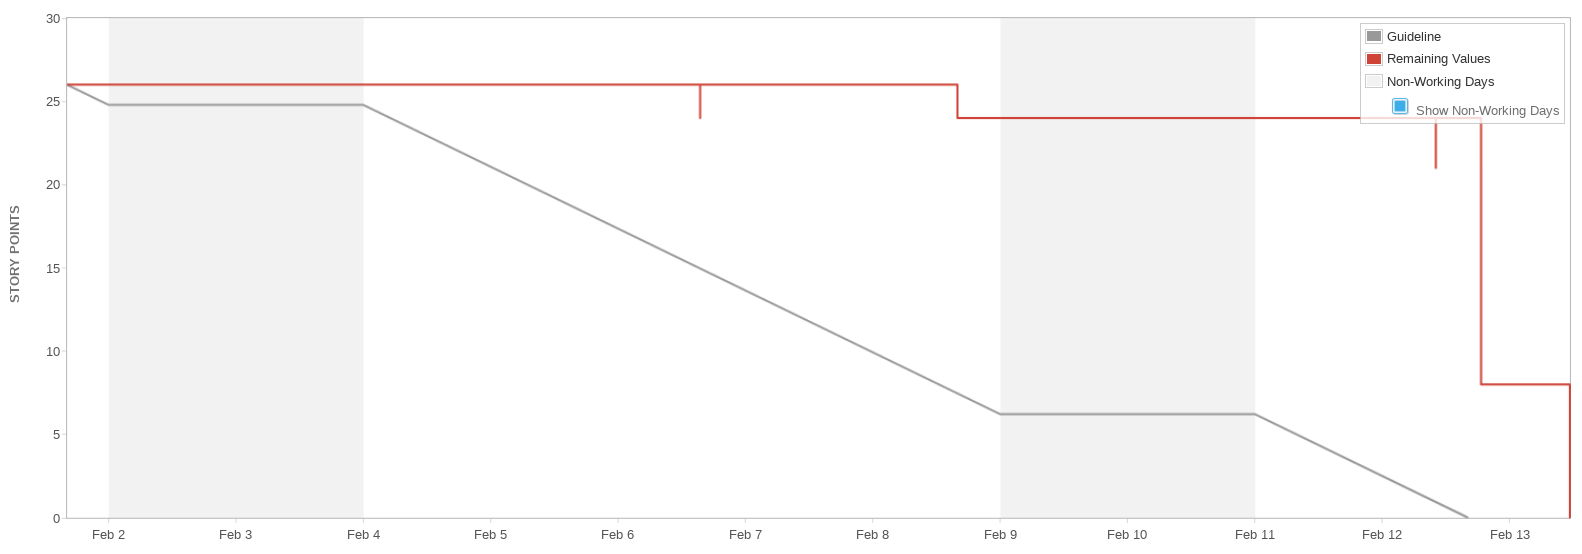
\includegraphics[width=\textwidth]{inc/images/sprints/sprintHelloWorld020219-130219.png}
    \caption{\Gls{burndown} chart for \gls{sprint} hello world.}
    \label{fig:sprintHellWorld}
\end{figure}

\newacronym{uri}{URI}{Uniform Resource Identifier}
\newglossaryentry{frontend}{name={front-end}, description={The presentation layer of a software}}
\newacronym{rest}{REST}{REpresentational State Transfer}
\newglossaryentry{webgl}{name={WebGL}, description={A JavaScript API for rendering interactive 2D and 3D graphics within any compatible web browser without the use of plug-ins \cite{wiki:webgl}}}


In this sprint the idea was to make a prototype that could represent a function definition from a \gls{git} repository \gls{uri}. The prototype should also indicate to the user if the browser does not support \gls{webgl}.

As figure \ref{fig:sprintHellWorld} shows, sprint took more time to finish than planned. The reason was that it took some time to get the parsed code to follow the planned \gls{json} format. This led to delays in visualizing it in the \gls{frontend}. \Gls{json} was a blocker for merging, once this was done all remaining task were completed.

\subsubsection{Front-end}
In \gls{frontend}, two \gls{html} pages were partially implemented; home page and visualization page.
In the homepage a field for submitting the \gls{git} repository link was created. If a valid repository \gls{uri} was submitted, user would be redirected to visualization page where loading would be shown. Once loading was completed a 3D visualization would be presented to the user.
There a representation of simple functions with random placement in 3D environment was implemented.

\subsubsection{Back-end}
In the \gls{backend}, \gls{api} \gls{rest} endpoints for initial request and adding \gls{git} repository link to database was implemented, along with java parsing for parts of simple function definitions. 

\subsection{Sprint: representation of complex data (14. feb - 18. feb)}
\begin{figure}[H] 
    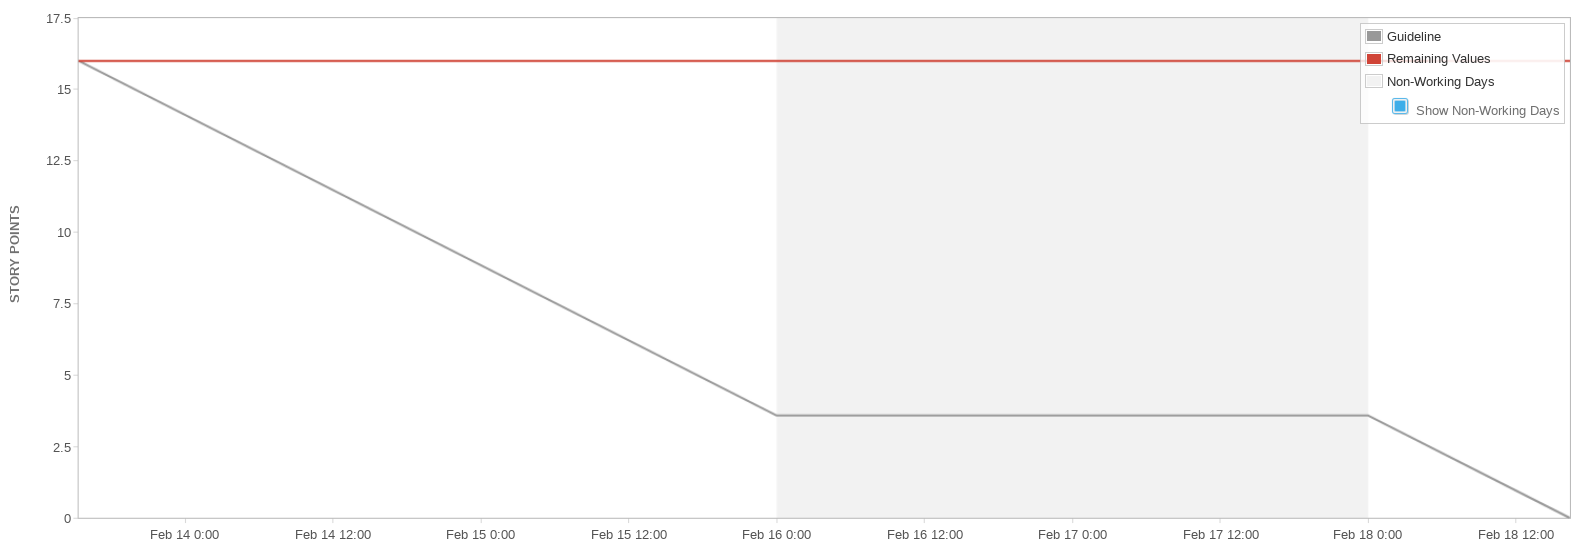
\includegraphics[width=\textwidth]{inc/images/sprints/sprintRepresentComplexData140219-180219.png}
    \caption{\Gls{burndown} chart for \gls{sprint} representation of complex data.}
    \label{fig:sprintRepresentationOfComplexData}
\end{figure}
\newacronym{gui}{GUI}{Graphical User \Gls{interface}}
\newglossaryentry{sourcecode}{name={source code}, description={Any collection of code, possibly with comments, written using a human-readable programming language, usually as plain text \cite{wiki:sourceCode}}}
The goal of the \gls{sprint} was to relate the visualization structure to its \gls{sourcecode} implementation and group together related structures.

Unfortunately no tasks were fully completed and all got transferred to the next \gls{sprint}. This is the reason for why the Actual Work Remaining line in Figure \ref{fig:sprintRepresentationOfComplexData} doesn't decrease within this \gls{sprint}. The tasks were underestimated and far too large to be completed.

\subsubsection{Front-end}
In the \gls{frontend}, the \gls{gui} for data structure implementation was failed to be integrated. Requirements for fulfilling this task were not satisfied. Therefore updating \gls{backend} was prioritized.
A basic version of \gls{fdg} that handles parenting relations of data structures was implemented but wasn't considered complete. \Glspl{namespace} were also only partially implemented.

\subsubsection{Back-end}
In the \gls{backend}, \gls{jap} was updated for function definition \gls{json} to include start line and end line for fetching its implementation. \Glspl{namespace} were also parsed.


\subsection{Sprint: interactable (20. feb - 25. feb)}
\begin{figure}[H] 
    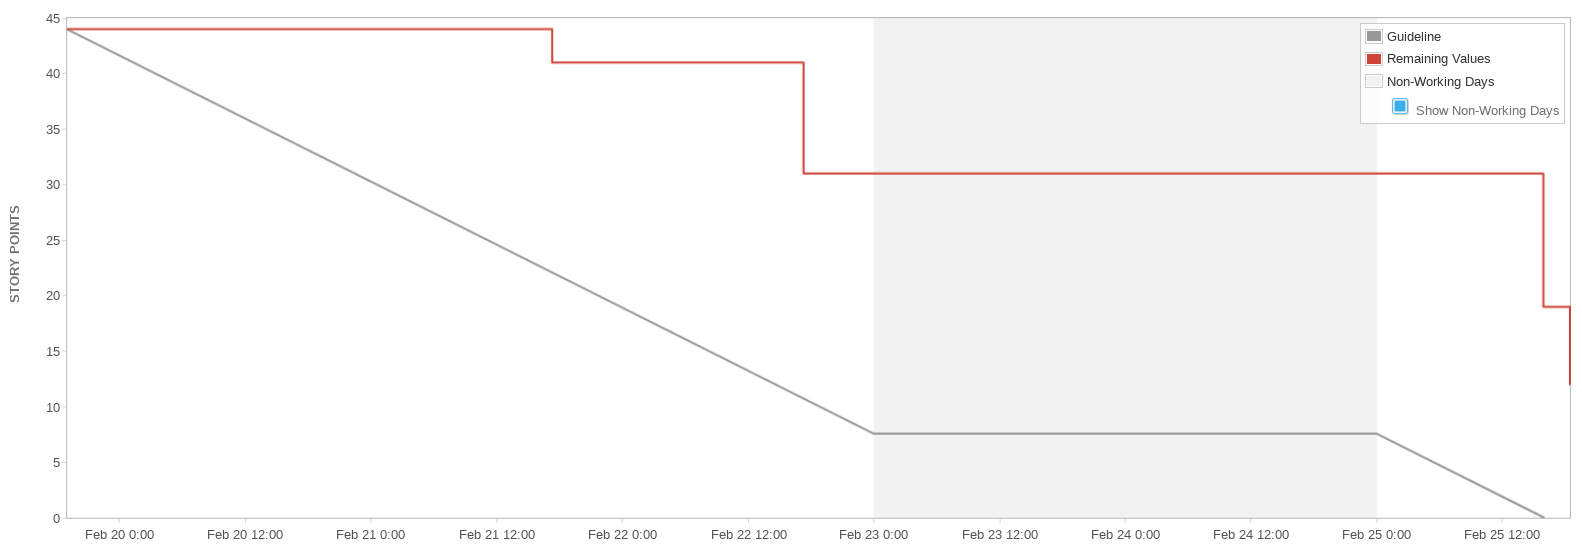
\includegraphics[width=\textwidth]{inc/images/sprints/sprintInteractable200219-250219.png}
    \caption{\Gls{burndown} chart for \gls{sprint} interactable.}
    \label{fig:sprintInteractable}
\end{figure}
The goal of this \gls{sprint} was to finish previous sprint, along with research on how to use \gls{antlr} for scope parsing. To improve on the previous \gls{sprint}, the tasks were divided more finely and declared more clearly.

\subsubsection{Front-end}
In the \gls{frontend}, the \gls{gui} layout of the system was implemented on the visualization page. Minor refactoring on \gls{frontend} was also done during this \gls{sprint}.

\subsubsection{Back-end}
In the \gls{backend}, was updated with a new \gls{api} endpoint for fetching implementation of functions. For \gls{jap}, through research the team found a recommended way to parse scopes from codebase using stack data structure \cite{parr2013definitive}. The task was underestimated and took some extra time to integrate the new implementation in \gls{jap}.

\subsection{Sprint: metadata and coupling (26. feb - 04. mar)}
\newglossaryentry{epic}{name={epic}, description={Large bodies of work that can be broken down into a number of smaller tasks \cite{atlassian:epic}}}
\begin{figure}[H] 
    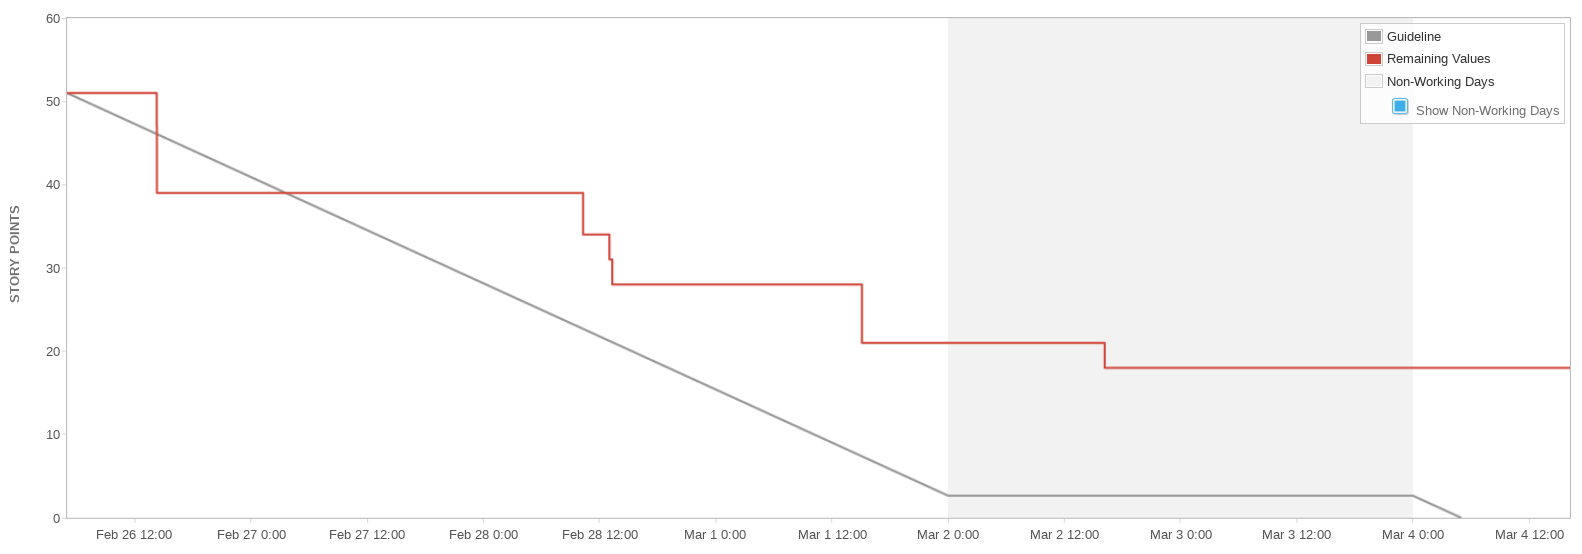
\includegraphics[width=\textwidth]{inc/images/sprints/sprintMetaData260219-040319.png}
    \caption{\Gls{burndown} chart for \gls{sprint} metadata and coupling.}
    \label{fig:sprintMetaDataAndCoupling}
\end{figure}
The goal of this \gls{sprint} was to add data about the project into the representation and visualize function calls.

Figure \ref{fig:sprintMetaDataAndCoupling} is a little misleading since it shows that the team was ahead of Ideal Work Remaining line. The reason Actual Work Remaining line dropped was that a task that should not have been in this \gls{sprint} was removed. From the previous \gls{sprint} the team also noticed that many tasks were \gls{fullstack} tasks and took a lot of time to finish. In this \gls{sprint} the team made \gls{fullstack} tasks into \glspl{epic}, divided them into stories and added sub-tasks under them so that the progress of the \gls{sprint} seemed continuous. The team also missed estimating sub-tasks which would have made the \gls{burndown} chart look even smoother. 

Some of the tasks in this \gls{sprint} were still big and depended on other tasks. Tasks such as display function calls was a very difficult \gls{fullstack} task that existed throughout all \glspl{sprint}. 

\subsubsection{Front-end}
In the \gls{frontend}, the team was able to connect the implementation window to show the implementation of simple function once clicked. Quality metrics window was also updated with simple metrics such as \gls{loc}, number of functions, classes and \glspl{namespace}. Repository window was implemented to show the repositories stored in the database, along with a \gls{rest} \gls{api} endpoint to fetch repositories.

\subsubsection{Back-end}
In the \gls{backend}, initial request functionality was updated to use \glspl{websocket}. This was done due to lack of information on processing of project files for the user on the loading page. Scope sensitive parsing was properly integrated in \gls{jap}.

\subsection{Sprint: complex parsing and relation (05. mar - 11. mar)}
\begin{figure}[H] 
    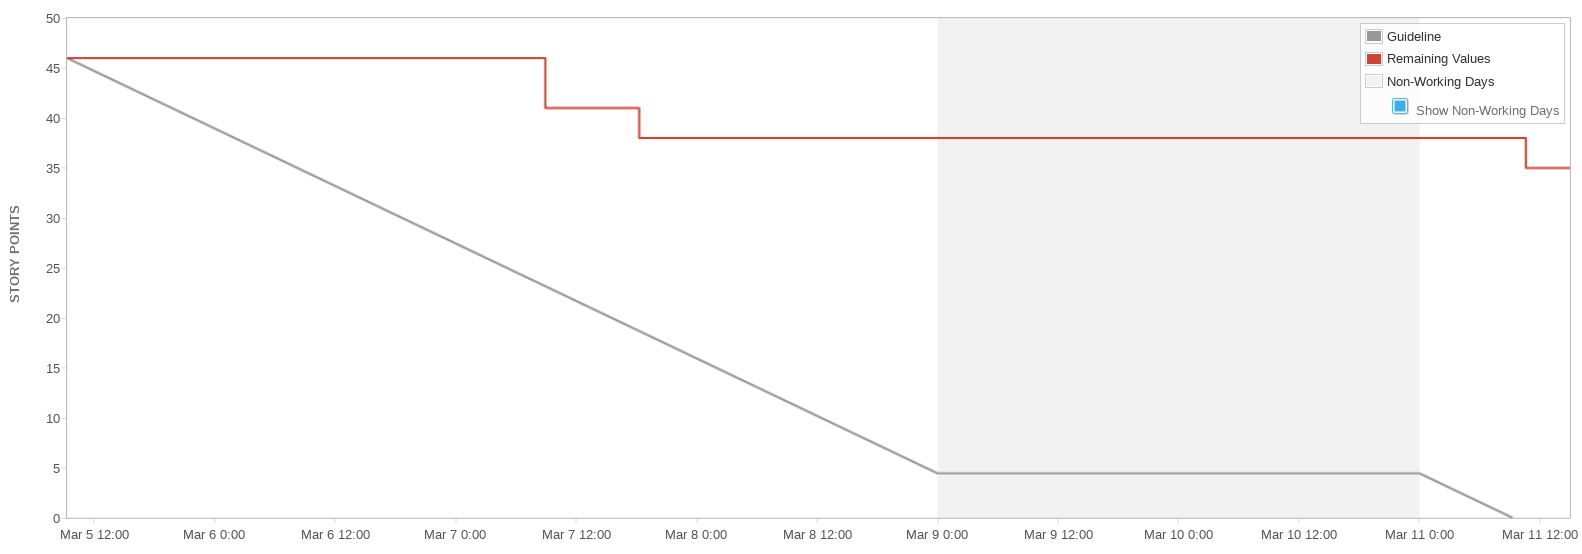
\includegraphics[width=\textwidth]{inc/images/sprints/sprintComplexParsingandRelation050319-110319.png}
    \caption{Burndown chart for sprint complex parsing and relation.}
    \label{fig:sprintComplexParsingAndRelation}
\end{figure}

The goal of this \gls{sprint} was to parse classes and continue improving parsing for function calls, in addition to research on quality metrics and measures.

\subsubsection{Front-end}
In the \gls{frontend}, the home page was updated with information on features completeness, browser support and contact information.

\subsubsection{Back-end}
In the \gls{backend}, \gls{websocket} was implemented.

The following were partially implemented or touched briefly due to other tasks having priority, which were too large and underestimated:
\begin{itemize}
    \item Parsing of classes for visualization.
    \item Parsing and extension of \gls{api} to include function calls for connecting related functions and classes.
    \item Research on complexity measures and applications/services that could perform these measures.
    \item View of implementation of functions.
\end{itemize}

This is also reflected in figure \ref{fig:sprintComplexParsingAndRelation}.

\subsection{Sprint: complex parsing and scope visual (12. mar - 18. mar)}     \label{subsection:SprintComplexParsingAndScopeVisual}
\begin{figure}[H] 
    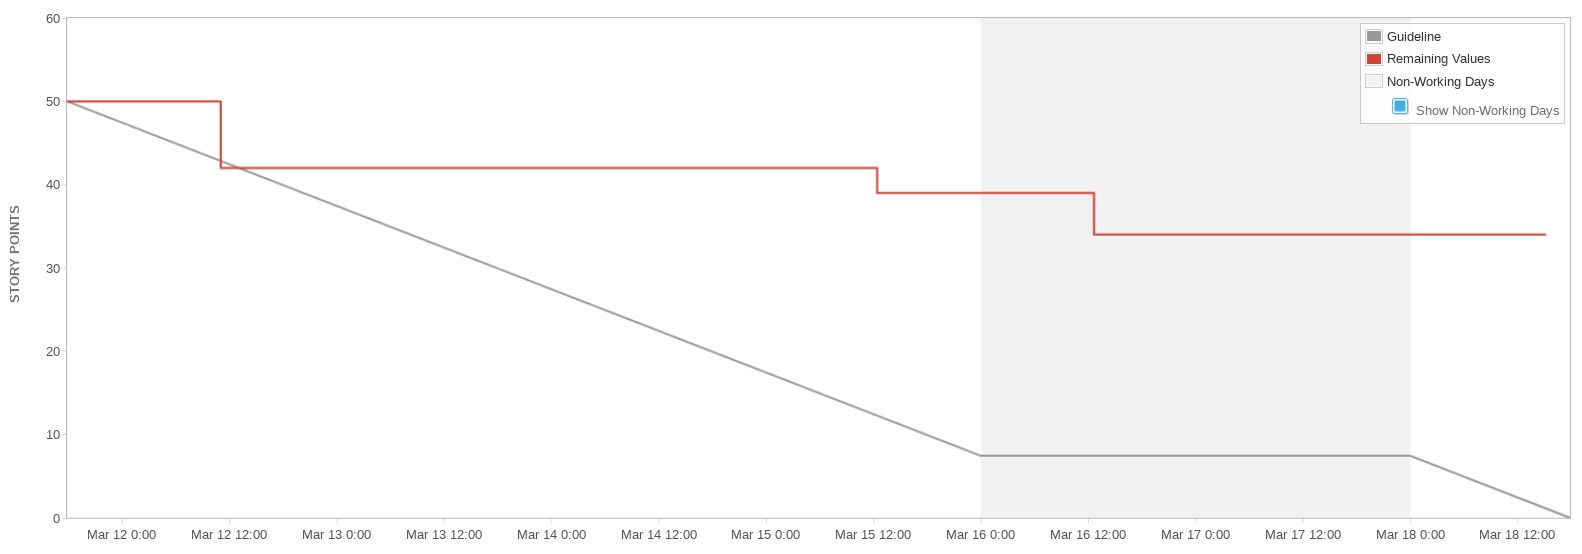
\includegraphics[width=\textwidth]{inc/images/sprints/sprintComplexParsingAndScopeVisual120319-180319.png}
    \caption{Burndown chart for sprint complex parsing and scope visual.}
    \label{fig:sprintComplexParsingAndScopeVisual}
\end{figure}
\newglossaryentry{planningPoker}{name={planning poker}, description={A consensus-based, gamified technique for estimating \cite{wiki:planningPoker}}}
\newglossaryentry{coupling}{name={coupling}, description={Is the degree of interdependence between software modules \cite{wiki:coupling}}}
\newglossaryentry{connacensemetrics}{name={connacense metrics}, description={A complexity measure for describing \gls{coupling} within a program}}
\newglossaryentry{cyclomaticcomplexity}{name={cyclomatic complexity},description={A complexity metric based on number of conditional or paths through a program}}
\newglossaryentry{halstedcomplexity}{name={halsted complexity},description={A complexity metric based on number of Operands, Operators and the total number of usages of each of these}}
\newglossaryentry{sonarqube}{name={SonarQube}, description={An open source platform to perform automatic reviews with static analysis \cite{sonarqube_2008}}}

The goal of this \gls{sprint} was to continue parsing function calls and visualize data structures within their respective scope.

As figure \ref{fig:sprintComplexParsingAndScopeVisual} shows, some tasks took very long to finish. This was due to underestimation as it was hard to conceptualize all aspects of the task during the \gls{planningPoker} session. This \gls{sprint} was one of the longest \glspl{sprint} the team went through, in total the team spent over 200 hours. The reason for this was that the team was extensively behind schedule and many of the core functionalities had yet to be figured out.

\subsubsection{Front-end}
In the \gls{frontend}, tree structures were used instead of arrays for \gls{fdg}. Implementation of tree structure was required before visualization of scopes could be done.
\subsubsection{Back-end}
In the \gls{backend}, Go \gls{api} endpoint for initial request was updated to give information about function calls. A custom logger was implemented in Go \gls{api}. Research on different quality metrics such as \Gls{connacensemetrics}, \Gls{cyclomaticcomplexity} and \Gls{halstedcomplexity} was done, along with finding an existing solution that could do static analysis on a specified code block. The team was recommended by supervisor to look into \gls{sonarqube} \gls{api}. This would have worked for our purpose but it would require a lot of configuration and was not done due to prioritization and time limitations. 
There was a lot of refactoring done in this \gls{sprint}. In \gls{jap} more listeners provided by \gls{antlr} were used instead of huge nested if statement blocks.  Parsing classes and function calls were partially implemented, but took multiple \glspl{sprint} to finish due to the flexibility of C++. The reason function calls took too long to finish is explained in more details in appendix \ref{appendix:retrospective2019-03-18}.

\subsection{Sprint: testing (19. mar - 02. apr)}
\begin{figure}[H] 
    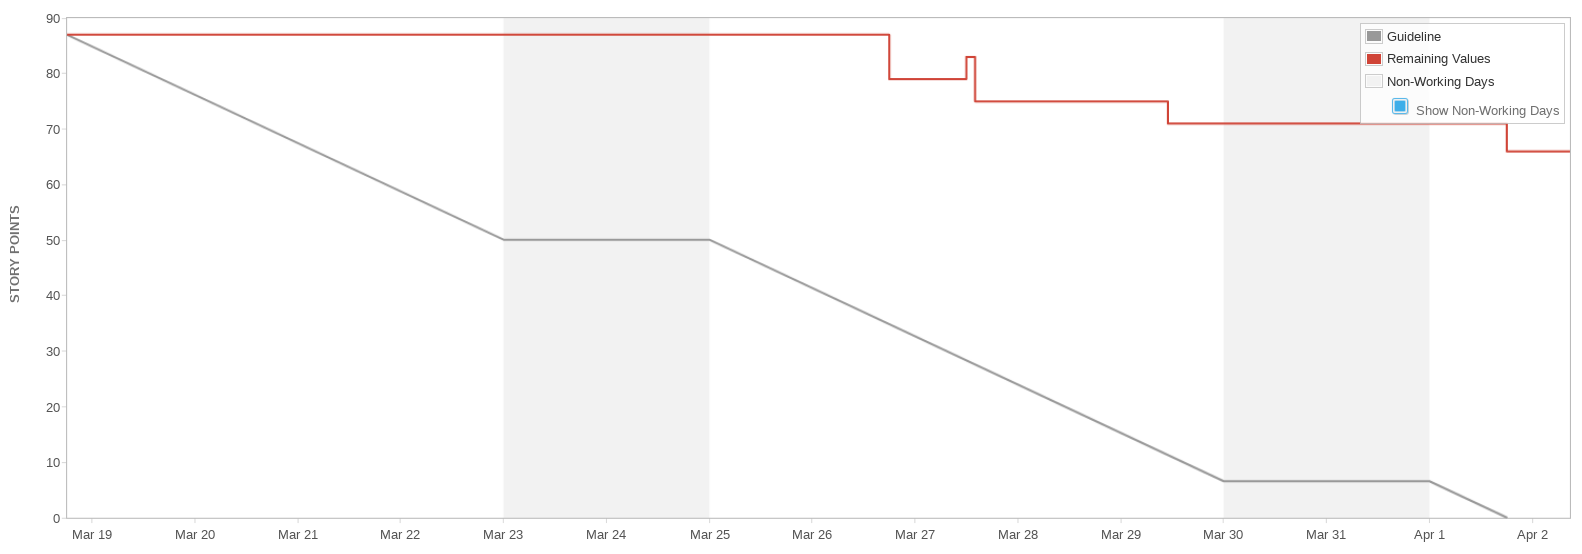
\includegraphics[width=\textwidth]{inc/images/sprints/sprintTest190319-020419.png}
    \caption{Burndown chart for sprint testing.}
    \label{fig:sprintTesting}
\end{figure}

\newglossaryentry{ava}{name={AVA}, description={Futuristic JavaScript test runner \cite{github:ava}}}
\newglossaryentry{junit}{name={JUnit}, description={A simple framework to write repeatable tests \cite{maven:junit}}}
This \gls{sprint} had a primary focus on testing and since no testing had been done and there were a lot of tests to write. Therefore it was decided to make this a two weeks long \gls{sprint}.

As the figure \ref{fig:sprintTesting} shows, no task was done in the first week and this is due to no experience with any of the testing framework that were used in this project such as \gls{junit} and \gls{ava}. 

\subsubsection{Back-end}
Tests in \gls{backend} were written for the following files and functionalities.
\begin{itemize}
    \item CodeSnippetController.go
    \item validation.go
    \item typeLogger.go
    \item repo/add - \gls{api}-endpoint
    \item Cpp and Java ParserFacade.java
    \item java Models
    \item MongoDB.go
\end{itemize}

\subsection{Sprint: complex task and testing (02. apr - 08. apr)}
\begin{figure}[H] 
    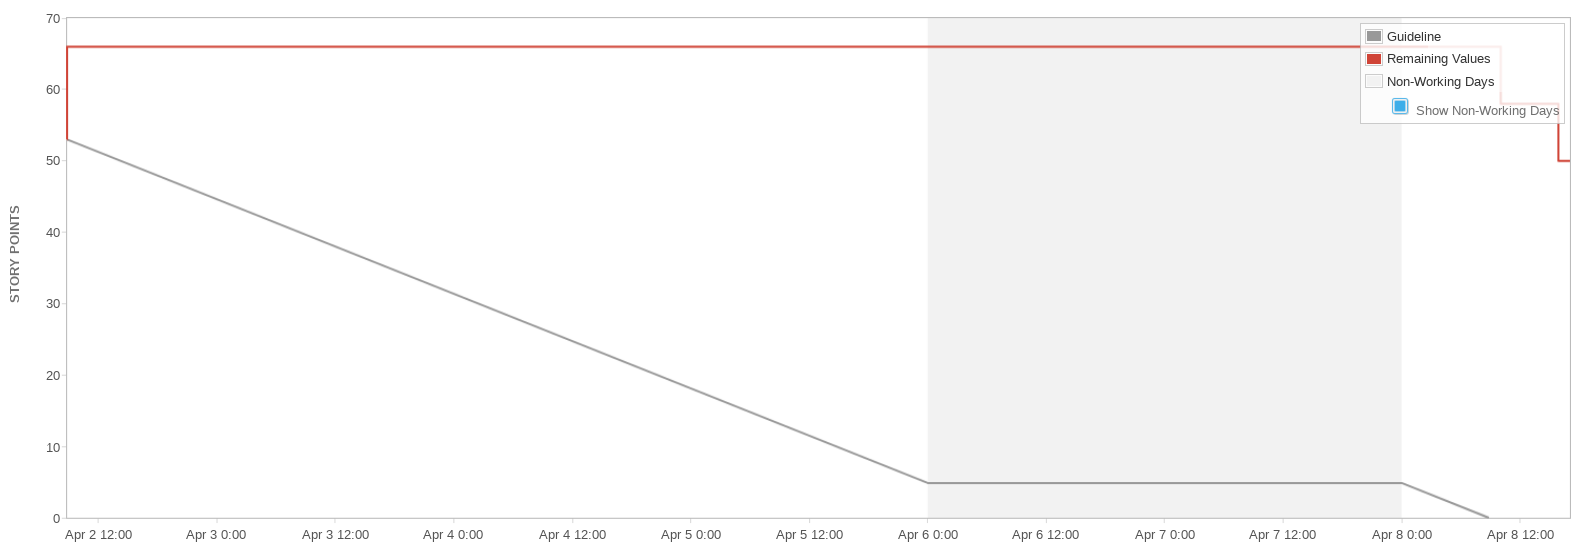
\includegraphics[width=\textwidth]{inc/images/sprints/sprintComplexTaskAndTest020419-080419.png}
    \caption{Burndown chart for sprint complex task and testing.}
    \label{fig:sprintComplexTaskAndTesting}
\end{figure}

This \gls{sprint} was a pair programming \gls{sprint} for tasks that were complicated and had existed throughout many \glspl{sprint}. Pair programming was very beneficial to get every group member up to date with the different components of the system that were initially implemented individually.
As the figure \ref{fig:sprintComplexTaskAndTesting} shows, it still took very long before the team could finish any task. This is due to the tasks in this \gls{sprint} being dependent on each other. The tasks were partially done before the team moved over to the dependent task and not finished before the end.
This made the pull request so large that the team were not able to accept it before the \gls{sprint} was completed.
Pair programming helped to get following task done;
\begin{itemize}
    \item In \gls{backend}, the \gls{jap} was updated with a complete implementation of class parsing, along with function calls parsing. 
    \item In \gls{frontend}, the visualization was updated with scopes inside scopes.
\end{itemize}

By the end of the \gls{sprint} some members felt that their time was better spent on individual tasks rather than pair programming.
\chapter{Implementation}
\label{chap:implementation}
%This has the description of how you actually went about implementing the project.  This should be focused on the interesting challenges and how those related to the project.

\section{Front-end web development}
\subsection{Overall design implementation}
\label{subsection:frontendOverallDesignImplementation}
%Explain the module pattern
\begin{figure}[h]
\noindent\rule{\textwidth}{1pt}
\begin{lstlisting}[language=JavaScript, caption={Use of Module pattern in stripped down FDG}, label={lst:module}]
var FDG = (function FDG(
    ...
    ) {
        ...
        var getNodeIndex = function(name) { ... }
        ...
        var getNodes = function() { ... }
        ...
        // Expose private functions for global use.
        return {
            getNodeIndex: getNodeIndex,
            getNodes: getNodes,
            ...
        }
    }
);
\end{lstlisting}
\noindent\rule{\textwidth}{1pt}
\end{figure}


% Team background oop.
The team have background in \gls{oop} and very limited experience with JavaScript. Implementation of \gls{frontend} started off as simple functionalities but become a problem as the team progressed. \Gls{frontend} was responsible of many thing such as \gls{fdg}, graphics, \gls{gui} and etc. It became a problem that code was expanding and the team did not know how to control files size but also how to properly divide the code sections in different files.
During refactoring team had done research and found different design pattern where module pattern \cite{scotch:javascriptpatterns} was very similar to classes encapsulation and felt a natural and easy choice to encapsulate functionalities in modern JavaScript fashion. One reason to choose module pattern was that the team wanted \gls{frontend} to be object-oriented, so that only the object would know about its properties and functionalities. Another reason to do so, is that it makes code easliy understandable by use of getters and setters functionalities, as shown in the figure \ref{lst:module}.
The team decided to implement module pattern to structure front-end code. 

There were two libraries used in \gls{frontend}, such as THREE.js and Imgui-js. Three.js is recommended \cite{cmarix:threejs} 3D graphics library as is based on WebGL. It also contains many different functionalities such as scenes, meshes, camera, lights and many more. This fits our requirements and worked for our purpose. Dear ImGUI is a windowing library for C++ that all team members are known of from graphics programming course \cite{course:graphics}. Dear ImGUI has a binding to JavaScript called ImGUI-js that uses TypeScript and Emscripten. This way we were able to integrate ImGUI-js into the system. The library is easy to use and fits our purpose.

\subsection{Force-directed graph}
The \gls{fdg} object maintains a tree of nodes and manage the inter-dependencies between nodes in the tree. It references the tree through its root, which in turn reference its children. The main force calculation and scope handling is done in nodes, so the \gls{fdg} functions as a wrapper.

\subsubsection{Position calculation}

\newglossaryentry{hookesLaw}{name={Hooke's law}, description={Describes a relationship between spring comression and force applied \cite{hooke1678}}}
\newglossaryentry{logit}{name={logit}, description={Inverse of the Sigmund function \cite{wordpress:logitandsigmoid}}}
\newglossaryentry{sigmoid}{name={sigmoid}, description={This is used to transform values on $(-\infty, \infty)$ into numbers on $(0, 1)$ \cite{wordpress:logitandsigmoid}}}

%Explain Logit and force. Could probably add graph from ProfProg rapport.
\begin{figure}[H]
\noindent\rule{\textwidth}{1pt}
\begin{lstlisting}[language=JavaScript, caption={Force calculation FDG}, label={lst:getTotalForce}]
    ...
    if (typeof link !== "undefined") { // Attractive forces
        forceScalar = (
            link.attraction * Math.log10(
                dist / (minDistance + size + node.getSize())
            )
        );
    } else {    // Repulsive force.
        forceScalar = (-1 *
            (
                (maxDistance + size + node.getSize()) /
                Math.pow(dist, 2)
            )
        );

    }
    ...
gravityForce = (Math.log10(distanceFromOrigin + maxSize) - Math.log10(maxSize - distanceFromOrigin)) * gravityForce;
...
\end{lstlisting}
\noindent\rule{\textwidth}{1pt}
\end{figure}

%// Attractive forces are based on logarithmic spring strenghts.
%// Repulsive forces are based on Hookes law (inverse square law).
To calculate the position, \gls{fdg} consider the root as the projects global scope, extracts its children and calculate the force between them. Each child is itself a scope within its parent. The force within each scope is calculated separately to assure that the structure stays within its scope. Listing \ref{lst:getTotalForce} shows that the force calculation depend on whether or not there is a link between the nodes. If there is a link, it is considered a positive attraction, otherwise it is considered a repulsion. 

The idea behind the attractive force calculation is a spring; more energy is required the further apart they are. \gls{hookesLaw} was considered for the calculation. The implemented calculation uses log on distance between each node divided by the minimum distance and size of each data-structure to create a repulsion when the two structures are too close and a strong attraction when they are far apart. 

The repulsion uses the inverse square law to grow weaker over a distance.

\begin{figure}
    \centering
    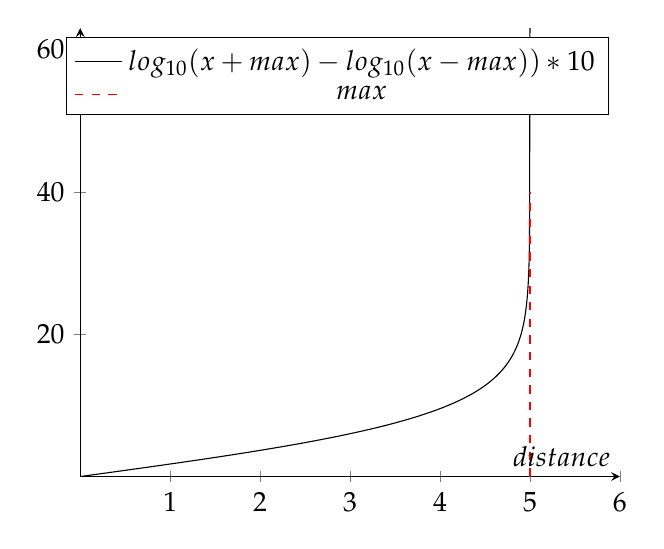
\begin{tikzpicture}
     \begin{axis}[ 
        xlabel={$distance$},
        ylabel={$force$},
        axis lines=middle,
        xmin=0,
        xmax=6,
      ] 
        \addplot[samples=1000, domain=0:5] {(log10(x + 5) - log10(5 - x))*10}; 
        \addlegendentry{$log_{10}(x + max) - log_{10}(x - max)) * 10$}
        
        \addplot +[mark=none, dashed] coordinates {(5, 0) (5, 40)};
        \addlegendentry{$max$}
      \end{axis}
    \end{tikzpicture}

    \caption{Gravity equation based on logit.}
    \label{fig:gravityPlot}
\end{figure}
The figure also show the gravity force calculation. Gravity attracts all structures towards the center of their scope. The center is the zero vector and updated with parents position when added to the scene graph after all relative positions have been calculated. The gravity calculation is based on \gls{logit}, as this implementation gives a gravity force approaching infinity when distance between structures approach max distance. This infinite force prevents structures from escaping their parent scope. The group choose to base it on \gls{logit} as the problem of limiting the position within a scope seemed related to \gls{sigmoid} that the group had experience with through REA1121 - Mathematics for Programming \cite{course:progMath}. \Gls{sigmoid} seemed relevant as it allowed for manipulation of the range and gave a smooth curve. Problem with \gls{sigmoid} is that if $x$ is distance and $y$ is force, then it would clamp on force rather than distance. \gls{logit} was described as the inverse of \gls{sigmoid} and would therefore clamp on distance, limiting the structure within its scope. As the distance between center and a structure could not be zero and gravity should never be negative, \gls{logit} was altered so it crossed the x axis at origin and approached infinity when it approached max distance like shown in figur \ref{fig:gravityPlot}.

\subsubsection{Recursivity of node}
\label{subsubsec:recuriviryOfNode}
%Explain the use of local/global index.
\tikzset{
    vertex/.style = {
        circle,
        fill            = black,
        outer sep = 2pt,
        inner sep = 1pt,
    }
}
\begin{figure}[H]
    \centering
    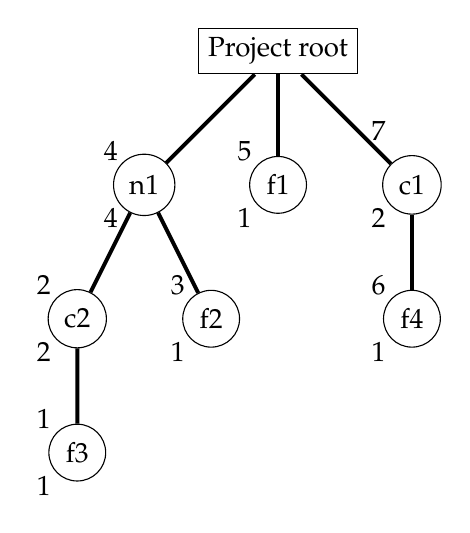
\begin{tikzpicture}[scale=0.85]
        % root
        %\node at (0.0, 1.0) {Project root};
        \node[draw] (root) at (0.0, 0.0) {Project root};
        
        %root scope
        %\node at (4, 1.0) {level 1}; 
        \node[draw, circle] (n1) at (-2, -2) {n1};       \draw[line width=0.5mm,draw=black] (root) to (n1);
        \node at (-2.5, -2.5) {4};    \node at (-2.5, -1.5) {4};
            \node[draw, circle] (c2) at (-3.0, -4.0) {c2};   \draw[line width=0.5mm,draw=black] (n1) to (c2);
            \node at (-3.5, -4.5) {2};    \node at (-3.5, -3.5) {2};
                \node[draw, circle] (f3) at (-3.0, -6.0) {f3};   \draw[line width=0.5mm,draw=black] (c2) to (f3);
                \node at (-3.5, -6.5) {1};    \node at (-3.5, -5.5) {1};
            \node[draw, circle] (f2) at (-1.0, -4.0) {f2};   \draw[line width=0.5mm,draw=black] (n1) to (f2);
            \node at (-1.5, -4.5) {1};    \node at (-1.5, -3.5) {3};
        \node[draw, circle] (f1) at (0, -2.0) {f1};    \draw[line width=0.5mm,draw=black] (root) to (f1);
        \node at (-0.5, -2.5) {1};    \node at (-0.5, -1.5) {5};
        \node[draw, circle] (c1) at (2, -2.0) {c1};     \draw[line width=0.5mm,draw=black] (root) to (c1);
        \node at (1.5, -2.5) {2};    \node at (1.5, -1.2) {7};
            \node[draw, circle] (f4) at (2.0, -4.0) {f4};   \draw[line width=0.5mm,draw=black] (c1) to (f4);
            \node at (1.5, -4.5) {1};    \node at (1.5, -3.5) {6};
        
        
    \end{tikzpicture}
    \caption{local to global index example}
    \label{fig:treeIndex}
    \medskip
    \small
    Figure shows a project with one namespace, one class and one function in global-scope, one class in the namespace and one function in each class. Top number is global-index and lower number is local-index.
\end{figure}
\begin{figure}[H]
\noindent\rule{\textwidth}{1pt}
\begin{lstlisting}[language=JavaScript, caption={Recursive to get node in tree, initiated by FDG(root)}, label={lst:getNode}]
    /**
     * Gets the node based on index.
     *
     * @param  {number} requestedIndex - The requested node index
     * @return {object} The node.
     */
    var getNode = function(requestedIndex, level){
        var localOffset = 0;                // Used to calculate relative index.
        var requestedNode = null;
        // Check if self is requested node.
        if (typeof index !== "undefined" && (index-1 === requestedIndex)) { 
            return this
        }
        // Check if children is requested node.
        children.every( function(child, i) { 
            localIndex = child.getIndex();
            // Check if requested is within childs range.
            if ((localIndex-1)+localOffset < requestedIndex){               
                localOffset += localIndex;
            }else {
                // Child cointain range with requested node.
                requestedNode = child.getNode(requestedIndex - localOffset);
                return false;
            }
            return true;
        });
        return requestedNode;       // indicate that node was not found
    }
\end{lstlisting}
\noindent\rule{\textwidth}{1pt}
\end{figure}
The \gls{fdg} tree requiers each node to have an identifier so that thy can identify each other for linking and potentially other purposes. This identifier is based on position in the tree and for easy searching. The identifier acts as an index in an array, starting at 0 and increasing with one for each node. When it was implemented, it had to be created based only on information of its sub-tree. This means its global index in the tree could not be calculated, only its local index where the node is the root. Once the tree is set in the \gls{fdg}, all nodes are given their global index. Before the global index is given, it can be calculated from the root node by using the local index given while building the tree. The local index is one greater than the sum of each child's local index. Figure \ref{fig:treeIndex} shows the relationship between local and global index while listing \ref{lst:getNode} shows a recurcive call to find a node with global index using the local index. LocalOffset in listing \ref{lst:getNode} refers to the offset from global index and local index caused by the parent node having a subtree to the left of the node being checked. Figure \ref{fig:treeIndex} is simplified by counting from  one instead of zero. The actual global index starts at zero to fit with array index. To account for the local index going from one and global index being accessed from zero, figure \ref{lst:getNode} shows index and local-index being subtracted by one in the conditionals.

\subsection{Localization}
\newglossaryentry{localization}{name={localization}, description={Translating a product into different languages or adapting a product to a country or region}}

\begin{figure}[H]
\noindent\rule{\textwidth}{1pt}
\begin{lstlisting}[language=JavaScript, caption={Language option functionality}, label={lst:locale}]
var LOCALE = (function() {
    var locale = {
        sentences: [
            {
                id: "language_not_found",
                values: [
                    {
                        language: "english",
                        value: "Could not find language"
                    },
                    {
                        language: "norwegian",
                        value: "Fant ikke spr\aket"
                    }
                ]
            },
            ...
        ]
    };

    // Available languages.
    const languages = ["english", "norwegian"];
    
    // English language as defualt.
    var currentLanguage = languages[0];
    
    var getSentence = function(id) { ... }
    ...
})();
\end{lstlisting}
\noindent\rule{\textwidth}{1pt}
\end{figure}

A common feature professional software includes to reach and benefit as many people as possible is \gls{localization} \cite{souphavanh2005localization}. To achieve this, a small system was implemented, where contributors could add sentences in specific languages to a \gls{json} structure, select a language in code and retrieve the added sentences. Even though the functionality for selecting the language exists, the \gls{ui} for selecting the language and updating the \gls{gui} in the visualization it self doesn't exists. The reason for this is that the \gls{gui} got a lower priority than the parsing and visualization. 

The current implementation of \gls{localization} is not very good due to the way sentences are stored. Sentences are stored as objects within a list, where each sentence has a list of the different languages and the sentence it self in that language. To find a sentence, one first have to find the correct sentence based on the identifier and then find the correct language based on the currently selected language. As more sentences are localized, the time taken to find the latter sentences is greatly increased due to the number of sentences to search through. A better way of implementing this would be to sort primarily on the languages them selves in a \gls{keyvaluemap}, where key is the language and value is a list of sentences. This would eliminate the use of list for languages and making the search process more effective. To optimize even further, the sentence list inside the \gls{keyvaluemap} could also be made into a \gls{keyvaluemap}. 

"getSentence" is the function responsible for fetching sentences in the currently selected language. If the sentence could not be found it defaults to the English language. 

\subsection{Graphics}
\label{subsection:graphicsFunctionLinking}
\newglossaryentry{scenegraph}{name={scene graph}, description={A collection of nodes in a graph or tree structure which arranges the logical and often spatial representation of a graphical scene \cite{dollner2000generalizedSceneGraph}}}

\begin{figure}[H]
\noindent\rule{\textwidth}{1pt}
\begin{lstlisting}[language=JavaScript, caption= {Linking function for calls}, label={lst:callLinks}]
var setLinks = function(tree, scene){
    scene.updateMatrixWorld();
    var nodes = tree.getSuccessors();

    nodes.forEach( function(node, index) {

        if (node.getDrawableIndex() != -1) {

            node.getLinks().forEach( function(strength, otherIndex) {

                if (nodes[otherIndex].getDrawableIndex() != -1) {

                    var material = new THREE.LineBasicMaterial({
                        color: STYLE.getDrawables().link.color
                    });

                    var geometry = new THREE.Geometry();

                    geometry.vertices.push(
                        new THREE.Vector3().setFromMatrixPosition(drawables.get(node.getType())[node.getDrawableIndex()].getMesh().matrixWorld),
                        new THREE.Vector3().setFromMatrixPosition(drawables.get(nodes[otherIndex].getType())[nodes[otherIndex].getDrawableIndex()].getMesh().matrixWorld)
                    );

                    var line = new THREE.Line(geometry, material);
                    scene.add(line);
                }
            });
        }
    });
}
\end{lstlisting}
\noindent\rule{\textwidth}{1pt}
\end{figure}

% The sequence of the paragraphs has to be looked at

% Introduce THREE.js?

% Scene graph
\href{https://threejs.org/}{THREE.js} uses a scene structure called \gls{scenegraph}. The structure in the \gls{scenegraph} allows to put object in a hierarchy and if the parent moves in the world, the children follow, to retain their position in relation to their parent. 

% Difficulties in linking
The \gls{scenegraph} caused a lot of confusion in linking the different functions based on calls. The solution for this was to use the \href{https://threejs.org/docs/#api/en/core/Object3D.updateMatrixWorld}{updateMatrixWorld} function from \href{https://threejs.org/}{THREE.js}'s \href{https://threejs.org/docs/#api/en/core/Object3D}{Object3D} which is the base class of \href{https://threejs.org/docs/#api/en/scenes/Scene}{Scene}. It runs a full update on all objects within the \gls{scenegraph} and updates all world positions. After this, it's possible to use \href{https://threejs.org/docs/#api/en/math/Vector3.setFromMatrixPosition}{setFromMatrixPosition} function from \href{https://threejs.org/}{THREE.js}, which uses the world matrix to calculate the actual position from world origin. 

Drawing of objects in \href{https://threejs.org/}{THREE.js} can be done by using the \href{https://threejs.org/docs/#api/en/objects/Mesh}{Mesh} object. This object takes a \href{https://threejs.org/docs/#api/en/core/Geometry}{Geometry} which is the shape made from vertices, and a \href{https://threejs.org/docs/#api/en/materials/Material}{Material} which gives the object characteristics and functionalities, e.g. Phong shading \cite{acm:phongShading1986article}, shadow mapping \cite{acm:perspectiveShadowMap2002article} capabilities, opacity, etc. These can then be added to the scene and updated if needed. 

The generation of the links is performed by looping over each nodes links and fetching the respective node's world position. These positions are given to a \href{https://threejs.org/}{THREE.js} \href{https://threejs.org/docs/#api/en/core/Geometry}{Geometry} and combined with a \href{https://threejs.org/docs/#api/en/materials/LineBasicMaterial}{LineBasicMaterial} object. This results in a line between the two positions. % Last sentence is probably unecessary

% Shapes
Within the visualization there are a bunch of shapes. Each shape represents some kind of data-structure, e.g. class, function, etc. Instead of building custom shapes, it was decided to use \href{https://threejs.org/}{THREE.js} built-in geometries. 

% Mention use of STYLE for color-scheme
The style feature is implemented in the same way as the localization. It contains a \gls{json} data-structure which has a list of color schemes and shape settings. The JavaScript Module pattern was used so the configuration data-structure could be encapsulated to maintain a god structure and keep the application as object oriented as possible. 

% More of a discussion section?
The group wanted the appearance of the application to be customizable to the different vendors, if they have a certain color scheme or style they follow or high contrast styles which highlights different aspects of the program better for those with visual disabilities. Colorblindness could be mitigated by using different shapes for the separate data-structures and a high contrast as well as colorblindness-specific color schemes. These color schemes are not currently implemented, but they will be if any work is continued. The only color schemes added are a SublimeText-inspired scheme and a CodebaseVisualizer3D-based scheme.

% Camera and lighting

\subsection{Interaction}
\newglossaryentry{raycast}{name={raycast}, description={The use of ray–surface intersection tests to solve a variety of problems in computer graphics and computational geometry. \cite{wiki:raycasting}}}

\begin{figure}[H]
\noindent\rule{\textwidth}{1pt}
\begin{lstlisting}[language=JavaScript, caption={A snippet of raycast onMouseClick}, label={lst:onClick}]
/**
 * On click mouse event function.
 *
 * @param      {Event}  event   The event.
 */
function onMouseClick(event) {

    // calculate mouse position in normalized device coordinates
    // (-1 to +1) for both components
    mouse.x = (event.clientX / window.innerWidth) * 2 - 1;
    mouse.y = - (event.clientY / window.innerHeight) * 2 + 1;

    // update the picking ray with the camera and mouse position
    raycaster.setFromCamera(mouse, camera);

    // calculate objects intersecting the picking ray
    var intersects = raycaster.intersectObjects(scene.children ,true);

    if(intersects !== "undefined" && intersects.length > 0) {
        var funcName = intersects[0].object.name.substr(0, intersects[0].object.name.indexOf(' |'));

        sendGetRequest("http://" + config.serverInfo.api_ip + ":" + config.serverInfo.api_port +
            "/repo/" + id + "/file/read/?lineStart=" + functionModels.get(funcName).getStartLine() +
            "&lineEnd=" + functionModels.get(funcName).getEndLine() +
            "&filePath=" + functionModels.get(funcName).getFileName())
        .then(json => {
            windowMgr.setDataStructureImplementation(json.implementation);
        });
    }
}
\end{lstlisting}
\noindent\rule{\textwidth}{1pt}
\end{figure}
\newglossaryentry{keyvaluemap}{name={key-value map}, description={An data-structure that maps keys to values}}
\newacronym{dom}{DOM}{Document Object Model}
The interaction that exists in the system is interaction with functions representations and windows. Window such as implementation window where data-structure implementation shown in it won't wrap but will be hidden and can be seen by temporarily expending it through clicking and dragging on the lower right corner of the window. Once released the window will reset to its original layout to not permanently hide the visualization.

The interaction with data-structures is done using a technique called raycast. Raycast is built into Three.js which is used for mouse picking objects from a 3d space. The function onMouseClick is added as an event listener to JavaScript built in window, which represents window containing \gls{dom} document. As the listing \ref{lst:onClick} shows, first the mouse position is normalized based on screen coordinates, then the raycaster is attached to camera and normalized mouse coordinates are given so that ray is casted from camera to mouse. Once the user clicks in the scene graph a list of intersected object with ray can be fetched. This list is sorted in the order objects were intersected by the ray. This way index 0 of the list will always be object user wants to interact with. The interacted object gives the name of the object that is assigned to object before its added to the scene. A \gls{keyvaluemap} of function models is created, whilst the project json is being parsed in \gls{frontend}. This \gls{keyvaluemap} contains all metadata about all functions that are visualized. This \gls{keyvaluemap} is used to identify the actual model the user has clicked. Once the actual function model is found, it can be used to fetch models implementation and visualize in the implementation window. 

\section{Back-end}

\subsection{Overall design implementation}
\newacronym{url}{URL}{Uniform Resource Locator}
\begin{figure}[h]
\noindent\rule{\textwidth}{1pt}
\begin{lstlisting}[language=go, caption={Api routes}, label={lst:apiRouting}]
// API routings
util.TypeLogger.Info("%s: Setting up api routes", packageName)
router.HandleFunc("/repo/add", controller.RepoController{}.NewRepoFromURI)
router.HandleFunc("/repo/list", controller.RepoController{}.GetAllRepos)
router.HandleFunc("/repo/{repoId}/initial/", controller.RepoController{}.ParseInitial)
router.HandleFunc("/repo/{repoId}/file/read/", controller.CodeSnippetController{}.GetImplementation)
\end{lstlisting}
\noindent\rule{\textwidth}{1pt}
\end{figure}
The \gls{backend} is divided into two parts as mentioned in Technical Design chapter; Go \gls{api} and Java \gls{antlr} parser.

As the listing \ref{lst:apiRouting} shows, some of the entry points has the repository ID as part of their \gls{url}. This \gls{url} path variable is sent from \gls{frontend} and is used to identify repository from database. The placeholder for repository ID is implemented using Gorilla Mux. The idea behind doing this was that the entry point would show what repository should \gls{api} deal with and what operation should be done on it based on \gls{url}. 

The ".../initial/" is the main request that uses \gls{websocket} and communicates with Java \gls{antlr} parser by giving a project file at a time, and expects a \gls{json} with parsed code in return. Whilst being parsed the \gls{frontend} will recieve a message about metadata of the file being processed through "onMessage" channel of \gls{websocket} for server feedback to user. In Go \gls{api} this \gls{json} is added into the project model. Once all project files are parsed the project model is converted into \gls{json} and will be sent as a response to "onClose" channel of \gls{websocket}. 

Initially the plan was to use \gls{antlr} in Golang for parsing and this would have worked since \gls{antlr} has binding for golang. Whilst the team was trying to integrate \gls{antlr} into golang, it came into focus that grammar files that the team was planning to use had embedded Java code, which would have not worked in Golang. Therefore Java seemed to be natural option to fallback to for parsing and since \gls{antlr} is natively made in Java. The team also had some experience in Java through mobile/wearable programming course \cite{course:mobileWearable} The package "os/exec" in Golang would be used to execute Java \gls{antlr} parser and read its output.

There are two library used in the \gls{backend} such as Gorilla mux and JSONObject.

Gorilla mux is a library that is widely used for \gls{url} routing for Golang projects. This library was mentioned in cloud technology course \cite{course:cloud} in which the team already had understanding of and made it very easy to integrate. 

In Java \gls{antlr} parser JSONObject library was used to construct \gls{json} for each data-structure model. Once every line in code is parsed the file model which contains many different properties such as namespace, will loop over each of
 
% endpoints

% gorilla mux as a librarary
% json in java


\subsection{Processing server in Golang}    \label{subsection:golang}

\subsubsection{REST and WebSocket}
\begin{figure}[H]
\noindent\rule{\textwidth}{1pt}
\begin{lstlisting}[language=Go, caption={Websocket success response}, label={lst:websocketMessageSuccess}]
response := WebsocketResponse{
	StatusText: http.StatusText(http.StatusOK),
	StatusCode: http.StatusOK,
	Body: map[string]interface{}{
		"id":               vars["repoId"],
		"status":           "Parsing",
		"currentFile":      parserResponse.CurrentFile,
		"parsedFileCount":  parserResponse.ParsedFileCount,
		"skippedFileCount": parserResponse.SkippedFileCount,
		"fileCount":        parserResponse.FileCount,
	},
}
\end{lstlisting}
\noindent\rule{\textwidth}{1pt}
\end{figure}
Initially the requirements asked for a \gls{rest} service, but this was loosened in favor of \gls{websocket} to allow for updating the user on progress of lengthy tasks. As \gls{http} responses has more extensive status information than \gls{websocket}, the team decided to use the responses as a wrapper for a trimmed down \gls{http} response with \gls{http}Status code, \gls{http}Status text and body containing the requested information. Listing \ref{lst:websocketMessageSuccess} shows a potential response to update user on status of code-base parsing. It sends \gls{http}Status 200 OK, along with what is being parsed, whether it is parsing, done parsing or has failed parsing, how many files have been found and the ration of files that were parsed or not. Files that are not parsed, might include README.md, \gls{git} files or files with unsupported extensions.  

\subsection{Language parsing in JAVA} \label{subsection:parsingJava}
\begin{figure}[H]
\noindent\rule{\textwidth}{1pt}
\begin{lstlisting}[language=AntlrGrammar, caption={Rule for memberdeclaration}, label={lst:antlrCppGrammarRuleExample}]
memberdeclaration
   : attributespecifierseq? declspecifierseq? memberdeclaratorlist? ';'
   | functiondefinition
   | usingdeclaration
   | static_assertdeclaration
   | templatedeclaration
   | aliasdeclaration
   | emptydeclaration
   ;
\end{lstlisting}
\medskip
\small
Taken from CPP14.g4 \cite{git:cpp14_g4} from the ANTLR grammar \gls{git} repository
\noindent\rule{\textwidth}{1pt}
\end{figure}

Listing \ref{lst:antlrCppGrammarRuleExample} shows the rule defining the syntax for member declaration. 
It specifies that it can be of 7 forms, where each is separated by a vertical bar or OR gate. The first rule specifies that it might contain an attributespeifierseq rule, followed by what might be a declspecifierseq, followed in turn by what might be a memberdeclaratorlist and ends with the ";" character. 

\begin{figure}[H]
\noindent\rule{\textwidth}{1pt}
\begin{lstlisting}[language=Java, caption={If block example}, label={lst:ifBlockExample}]
	protected boolean isVariable(CPP14Parser.SimpledeclarationContext ctx){
		CPP14Parser.InitdeclaratorlistContext initDeclList = null;
		CPP14Parser.DeclaratorContext declarator = null;

		if(ctx.initdeclaratorlist() != null) {
			initDeclList = ctx.initdeclaratorlist();
			if(initDeclList.initdeclarator().declarator() != null) {
				declarator = initDeclList.initdeclarator().declarator();
				if(declarator.ptrdeclarator() != null) {
					if(declarator.ptrdeclarator().noptrdeclarator() != null) {
			            if(declarator.ptrdeclarator().noptrdeclarator().declaratorid() != null) {
							return true;
						}
					}
				}
			}
		}

		return false;
	}
\end{lstlisting}
\noindent\rule{\textwidth}{1pt}
\end{figure}
As the grammar file defines the structure of the program, it was highly desired that as much of the parsing as possible be handled by \gls{antlr}. If \gls{antlr} handled the scoping and definitions then one could be very certain that no data-structure was skipped or mishandled. Listing \ref{lst:ifBlockExample} shows an example of where checking for variables is done manually, rather then relying on more listeners in given by \gls{antlr}. This can create a lot of nested if statements to check what form of the rule or nested rule is being matched. This increase the \Gls{cyclomaticcomplexity} and probability of error while also relying on the development team knowing all the niche aspects of a particular data-structure structure. The same is true when merging the output of rules by defining an interval by using the the start point of a rule and the endpoint of an other. If there are optional rules within the context, then the output can vary greatly. 

% More talk about rules?

\begin{figure}[H]
\noindent\rule{\textwidth}{1pt}
\begin{lstlisting}[language=Java, caption={Antlr CPP listener example}, label={lst:antlrCPPListenerExample}]
public void enterFunctiondefinition(CPP14Parser.FunctiondefinitionContext ctx) {
	...

	FunctionModel functionModel = new FunctionModel(input.getText(interval));
	functionModel.setLineStart(ctx.functionbody().start.getLine());
	functionModel.setLineEnd(ctx.functionbody().stop.getLine());
	this.enterScope(functionModel);
}

public void exitFunctiondefinition(CPP14Parser.FunctiondefinitionContext ctx) {
	Model model = this.exitScope();

	if (model instanceof FunctionModel) {
		this.scopeStack.peek().addDataInModel((FunctionModel) model);
	} else {
		this.enterScope(model);
		... // Print wrong parent model
	}
}
\end{lstlisting}
\noindent\rule{\textwidth}{1pt}
\end{figure}
\begin{figure}[H]
\noindent\rule{\textwidth}{1pt}
\begin{lstlisting}[language=Java, caption={Antlr Java listener example}, label={lst:antlrJavaListenerExample}]
public void enterMethodDeclaration(Java9Parser.MethodDeclarationContext ctx) {
	...// Get interval were function identifier is written.
	
	FunctionModel functionModel = new FunctionModel(input.getText(interval),
			ctx.methodHeader().methodDeclarator().identifier().getText());
    functionModel.setLineStart(ctx.methodBody().start.getLine());
	functionModel.setLineEnd(ctx.methodBody().stop.getLine());
	this.enterScope(functionModel);
}

public void exitMethodDeclaration(Java9Parser.MethodDeclarationContext ctx) {
	Model model = this.exitScope();

	if (model instanceof FunctionModel) {
		this.scopeStack.peek().addDataInModel((FunctionModel) model);
	} else {
		this.enterScope(model);
		... // Print wrong parent model
	}
}
\end{lstlisting}
\noindent\rule{\textwidth}{1pt}
\end{figure}

Listing \ref{lst:antlrCPPListenerExample} and \ref{lst:antlrJavaListenerExample} shows a trimmed down version of the parsing of function definition in C++ and Java respectively. Parsing of the two languages can differ significantly as the naming convention used in the different \gls{antlr} grammar files differ and C++ also has a more flexible syntax. Java grammar might also use different methods for defining lists than C++. 
Due to the differences in Java and C++, they are handled separately based on the file extension. 

Java is read by the JavaParserFacade and interpreted by JavaExtendedListener, while C++ is handled by CppParserFace and CppExtendedListener class. Each of the extended listeners extend from their respective \gls{antlr} listener and are meant to contain common functionality for all types of parsers for their language. Currently only the initial parsers exist. The initial parsers create the initial data used for the main project visualization. 

Both \ref{lst:antlrCPPListenerExample} and \ref{lst:antlrJavaListenerExample} listings show the enter function ending with the enterScope(functionModel) call and the exit functions calling exitScope. The enter function is called when the parser reaches the beginning of its respective rule while the exit is called at the end. With the enterScope being called, all following rules being called would have functionModel in memory and know they are matched within the function rule. The check for whether or not the instance of the model is of the expected type in the exit function, were initially undesirable as with a correct and full implementation of the \gls{antlr} file, there would be no possibility for an unexpected model.

%This is for those you will actually be getting code out beyond the end of the thesis.  This describes how the code is deployed on the test servers and into the testing environment.  Having the code running on your own machines is nice, but you need a process so that you can share your code with other people and have it actually run without them having to have a copy of a compiler and recompile your code.

\chapter{Deployment}
\label{chap:deployment}

\section{Dockerization}
\newglossaryentry{mongo}{name={MongoDB}, description={A document database storing data in \gls{json} like documents \cite{mongodb}}}

\Gls{docker} was used to simplify the system setup for any administrative users and help with documenting the infrastructure. The goal was to be able to launch the system by running the command: "docker-compose up".

With this it would be easier for potential administrators to test the system and figure out if it would be appropriate for their use-case. It would also be easier to continue with \gls{opensource} development, as the \gls{docker} instances could be used as a common test bed. 

\Gls{dockercompose} names four services:
\begin{itemize}
    \item web - Serves the \gls{html}, \gls{css} and \gls{js}. Mainly deals with the visualization, presenting state and quality metrics.
    \item api - The Go \gls{api} server. Mainly dealing with controlling the database and parser on requests from web. 
    \item  mongo\_db - The \gls{mongo} database \cite{mongodb}.
    \item doc - Serves the \gls{apidoc} 
\end{itemize}

The services; web, api and doc each have a defined \gls{dockerfile} in the repository, while mongo\_db uses mongo:latest, which is the official image. 

mongo\_db is connected with api but not with the network. This improves the security by not directly exposing the database to the internet.

\section{Deployment on SkyHigh with HOT}
\newglossaryentry{openstack}{name={OpenStack}, description={A cloud operating system that controls large pools of compute, storage, and networking resources throughout a datacenter\cite{openstack}}}
\newglossaryentry{skyhigh}{name={SkyHigh}, description={\gls{openstack} instance hosted by NTNU}}
\newglossaryentry{jenkins}{name={Jenkins}, description={A self-contained, open source automation server which can be used to automate all sorts of tasks related to building, testing, and delivering or deploying software. \cite{jenkins}}}
\newacronym{hot}{HOT}{Heat Orchestration Template \cite{openstack:hot}}

As of the writing of this report, the system is deployed at \gls{skyhigh} and associated with the domain \url{http://www.covi.tech/}.

It uses \gls{hot} to automate the server setup process. The template defines three servers:

\begin{itemize}
    \item development - Meant as a testing server that updates rapidly and might contain bugs.
    \item operations - Meant to be used by the end users and updated with each milestone where most bugs have been patched.
    \item master - Meant to run \gls{jenkins} to automate updates of development and operations.
\end{itemize}

Due to the teams very limited experience with \gls{openstack} and \gls{jenkins}, the servers were rarely updated and down prioritized as it would require more time to learn than what could be allocated. 
\chapter{Testing and User Feedback}
\label{chap:testing}

\section{Unit testing}

\begin{figure}[h!] 
    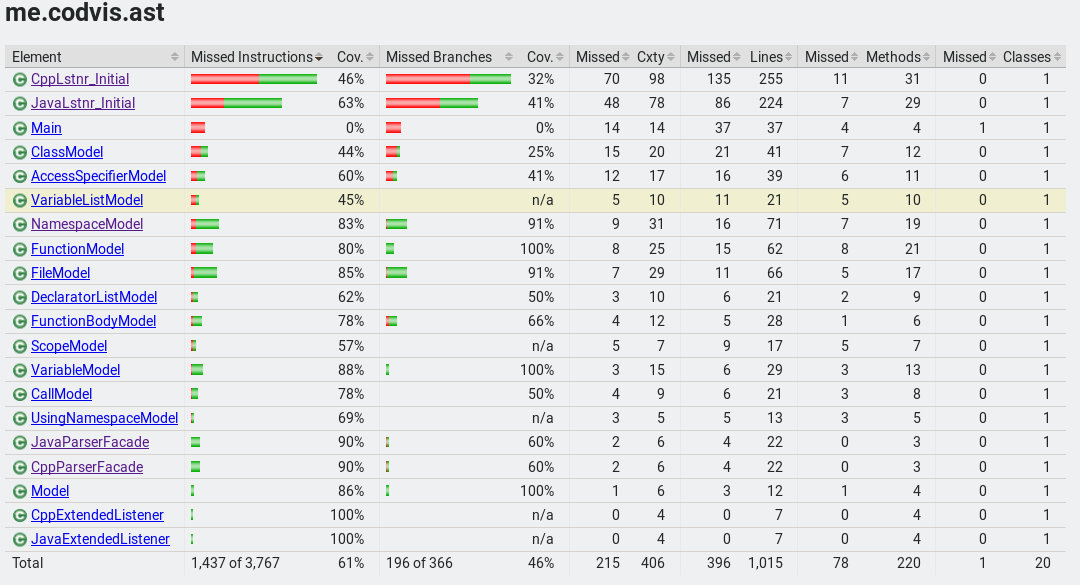
\includegraphics[width=\textwidth]{inc/images/test/JavaTests.png}
    \caption{Test summary of different Java \gls{antlr}  parser files.}
    \label{fig:testJava}
\end{figure}


Unit testing was done in Java \gls{antlr} parser using JUnit. In Java \gls{antlr} parser unit tests were written for most of the models and listeners. 
The goal of unit testing was to test as many as possible instructions. Trivial functionalities such as getters and setters were not tested.
Each model is tested to see if only data of compatible types would be inserted and would return the correct data once asked for \gls{json}. Listeners were tested to see if they were able to parse specified context and were able to create correct models that could return correct data within \gls{json}. Testing in Java was not complete due to prioritization of other important tasks. 

\begin{figure}[H] 
    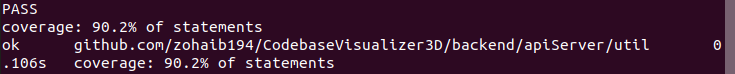
\includegraphics[width=\textwidth]{inc/images/test/apiServer_testCoverage_util.png}
    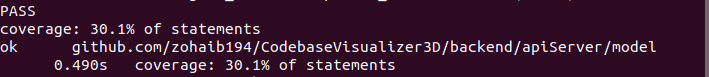
\includegraphics[width=\textwidth]{inc/images/test/apiServer_testCoverage_model.png}
    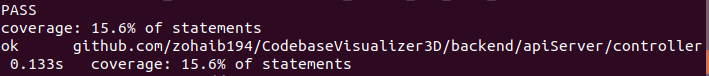
\includegraphics[width=\textwidth]{inc/images/test/apiServer_testCoverage_controller.png}
    \caption{Test summary of different Go \gls{api} files.}
    \label{fig:testGO}
\end{figure}


In Go \gls{api} the goal was to test the \gls{api} entry points through \gls{frontend} using a \gls{js} testing framework called \gls{ava}, but functionality used for entry point within Go should be test using Go test. As shown in figure \ref{fig:testGO}, util package is a custom package for different logging functionalities that are used through out the Go \gls{api} and almost all functionalities are unit tested. In model package only the database functionalities are tested. In controller package one of the REST endpoint was tested. This happened before the goal of testing in Go \gls{api} was set. The endpoint accounts for multiple good and bad tests cases. To create a general structure in testing code for Go a sublime package was used called gotests \cite{github:gotestsplugin}.

\begin{figure}[H]
\noindent\rule{\textwidth}{1pt}
\begin{lstlisting}[language=JavaScript, caption= {JSON structure for a valid test case}, label={lst:testCase}]
{
	name: "Valid - new repo - sendAddRequest",
	websocketURL: "ws://localhost:8080/repo/add",
	payload: {
		uri: "https://github.com/example/ECS.git"
	},
	wantMessage: {
		length: 1,
		messages:
		[
			{
				statuscode: 202,
				statustext: "Accepted",
				body : {
					status: "Cloning"
				}
			}
		]
	},
	wantCloser: {
		reason: {
			statuscode: 201,
			statustext: "Created",
			body: {
				status: "Done"
			}
		}
	}
}
\end{lstlisting}
\noindent\rule{\textwidth}{1pt}
\end{figure}

In \gls{frontend} only one of the end points were able to be tested due to time prioritization. The endpoint is implemented as \gls{websocket} and as shown in the listing \ref{lst:testCase}, \gls{json} structure was used as for a test case. This test would add a new repository link and expects onMessage and onClose channel of \gls{websocket} to receive data as shown.

\section{Code Quality}
The team put a lot of effort looking into professionalism and best practises when it comes to code. To maintain high code quality there were a number of steps taken:

\begin{itemize}
    % Merge request issues
    \item Merge requests in Github was used so any members code would be looked through by at least one member and errors would be reported and not merged until resolved. This was also very helpful in the sense of giving all members a peek into progress and what was done in the areas not touched by them. 
    % Documentation
    \item Documentation were prioritized throughout the project both commenting for auto-generated documentation but also self-documenting code.
    % Convensions and Best practises
    \item Conventions and Best practises were also prioritized. They are always good to follow because they are tried and tested informal rules to produce easily maintainable and high quality code \cite{wiki:bestCodingPractises}. 
    % Dependency quality assurance
    \item Dependencies, inspiration and ideas were taken form what the team considered professional grade projects, libraries or frameworks. If they are still active in development or maintenance, any recent updates, number of people who contributed, general good structure and open-source were all items we would check for on any project to determine whether it was created in a professional setting. For example if a project has one contributor or significantly lacking in number of commits for the apparent level of complexity, it would not be considered as a professional grade project unless the code itself is regarded as being good. % Kent: Contradictory? Too much repetition? Too segmented?
\end{itemize}

\section{User studies}
User studies are very important in the sense that it's a controlled trial of the application. The developers can get an insight into how the users will use the application and give feedback on improvements. This usually results in a higher quality product and the developers can ensure that the application is easy-to-use and stable \cite{kosara2003user, sridhar1995understandingTheUser}. As this project is more of a research based project, much of the application is more of a prototype and might not be intuitive. The group therefore performed a user study that is available in Appendix \ref{app:userStudies} to get some ideas on how to improve the system. 

\subsection{User categorization}
The users of this application are categorized in to three types, Student, Lecturer and Professional: 
\begin{itemize}
    \item Student is anyone looking up a library for any number of reasons. 
    \item Lecturer is anyone trying to teach something about a concept and uses this application for this purpose. 
    \item Professional is anyone using the application in any professional or corporate setting.
\end{itemize}

The intended result from this classification is that the different groups will have different ways of viewing the application. Students might have a more simplistic view and initial understanding of the system and might therefore focus more on usability and basic functionalities. Lecturers might be more analytical and will focus a little more on what the system will give them, how it gives this information and why its represented the way it is. The professionals might view the application from a industrial perspective and might give feedback about \gls{it} related industrial standards, quality and more advanced features.

\subsection{Testing methodology}
\newacronym{gdpr}{GDPR}{General Data Protection Regulation}
Before the participant answer the questions in the questionnaire, they're instructed to look at a predetermined code-example and asked to draw their visualization that represents the given code-example, as well as some basic tasks that will probe how they use the application. Information like where they look to improve efficiency of retrieving information, mouse movements to see indications on though process and any control inputs to look for navigability issues and intuitiveness within the visualization.

The primary reasons for selecting these questions is that some will give insights into how the application is used and how easy it is to retrieve any additional information from the home page. Others will probe the visualization it self and give an insight to whether it's intuitive and easy to navigate. Some questions will probe the GUI within the visualization and it's layout for retrieving/viewing any information and others will give a general understanding of their role but will not be sufficient to identify the individual.

In a in-formal user study it's important that one doesn't break any \gls{gdpr} laws which means no recording of any data that can identify the person testing the application without users consent, the ability for the user to request or delete their data and that is deleted within reasonable time. \cite{lovdata:gdpr}. 

\section{Results}
As the user study only involved nine participants, the data is not extensive enough to make any definitive conclusions, the group is however confident that data gathered could still be used to guide future work. 

\subsection{Navigation and UI}
The questionnaire indicated that the users felt the navigation was mostly intuitive, but wanted information on how it worked rather than leaving it to guesswork. The activities however, indicated that many of them struggled and did not see it as intuitive, especially moving into the data-structures and sideways movement. One thing that seemed clear was that initial camera position, before moving, was too close. This made it difficult for the user to orient themselves. It was also mentioned by a user that information about current orientation would be beneficial.

Several users tried to use the static windows for navigation. This was a feature the team had previously thought about, but had not implemented due to time constraints. It became clear that this should have been prioritized higher.

\subsection{Visualization and interaction}
Most users indicated that the choice of colors and shapes were good, and had little problem identifying the relationship between the visualization and code. 

Several users had problems with finding the implementation, whether this had to do with unclear terminology or if changes made by the interaction was hard to spot is unclear. Most users clicked the function to get the implementation as expected, but some did not notice the update in the separate window or noticed but did not draw the connection. An improvement might be to add syntax highlighting, increase the size of the window or highlight to active function in the visualization.

\subsection{Proposed features}
\begin{itemize}
    \item Information about how to navigate
    \item Information about orientation
    \item Customized navigation option
    \item Save and restore camera position
    \item Ability to change visuals
    \item Sidebar navigation
    \item Position reset button
    \item Toggle visibility
    \item Information about call order
    \item Integrate source code into visualization
\end{itemize}

Most of the suggestions had been discussed earlier and was planned if time allowed for it, but there seem to be a higher want for enhanced navigation features than expected. 
\chapter{Discussion}
\label{chap:discussion}

\section{Overall reflection and experience}

Initially the group wanted to keep very high standards for code quality and professionalism. Although all still strove for this throughout the project the team quickly fell behind schedule, therefore sacrificed on professionalism in order to get working features and ensure scalability. The parts of professionalism that suffered was mostly documentation of the process and unit tests. Part of why the documentation did not stand up to what was suggested in the project plan as shown in the appendix \ref{app:projectPlan}, was that the project plan template did not fit highly \gls{agile} workflows like the group followed. The group followed \gls{scrum} and had documented sprint retrospective and sprint planning meetings, but the low communication threshold meant that most planning was done verbally and not through writing. It allowed for rapidly changing ideas and refactoring, but very little code that could be considered final and therefore not considered worth writing tests for. This will make it more difficult for potential \gls{opensource} developers to take over afterwards. Although it is unlikely that others will continue the project it still seemed like a valid compromise.

The low communication threshold meant that those working on relatively complex tasks would ask for a second opinion or ideas for potential solutions. This in turn meant that each group member felt committed and prioritized the more advanced tasks. This was beneficial and helped to solve some of the tasks that could not have been solved by an individual. This also had the negative effects of down prioritizing less complex tasks that could easily give a slight enhancement to the project and that the groups focus could slip. The groups would talk about project unrelated topics more than what was considered optimal and therefore had to spend more time than what was expected. Time log can be found in appendix \ref{app:timelog}.

It was often mentioned that progress was behind schedule set in the project plan, although the schedule comment specifically mentioned that changes were expected and should be embraced. It is good that this pushed for quicker development, but it might also have harmed the scalability of the project and thereby also slowed it down by pushing for features when the plan was not fully formed. 

The group was always aware that the project was complicated and required a lot of research and experimentation, but throughout the development it seemed that group members did not expect the same level of completeness. The product owner had at some occasions described the project as a research project, yet the supervisor mentioned that the project requirements should be written as hard requirements, something that conflicted with both the research based and agile nature of the project.

Overall impressions is as expected, the group knew the project was very ambitious and aimed more for an idea than a realistic goal. This meant the learning outcome would be significant and pushed the team to do better than what was realistic. It was hard work, but still very interesting and as a group there was a genuine belief that all members would want to continue developing the project after the thesis was finished.

\section{Use of Jira}
\newglossaryentry{toggl}{name={Toggl}, description={A time tracking app \cite{wiki:toggl}}}
Throughout the project the team used \gls{jira} for managing the backlog, sprints and the planning of tasks within these sprints. Some tasks at the start were quite large and required Full-Stack development, e.g. "As a user I would like to see classes parsed and visualized in 3D". These tasks are far too big, especially for the group who has very limited experience with technologies used like \gls{antlr} and \gls{js}. The individual group members would also spend a whole week on the same task and this felt quite daunting after a couple of weeks. The group then decided to make these tasks into epics and segment them down into user-stories and sub-tasks. This made the tasks more finely defined and easier to tackle. This made the group members individually more motivated and made the development process feel less daunting, because a member could complete more tasks in a shorter period of time, therefore gain more satisfaction in seeing multiple tasks getting completed. The break-down of the tasks also had the added benefits in making the burn-down charts look more professional and would more accurately represent the work being done. Despite this, underestimation was still a severe problem and some stories were not estimated due to \gls{jira} treating sub-tasks, stories and epics differently. The \gls{planningPoker} tool in \gls{jira} worked well for estimating stories, but had problems with subtask. Subtasks did not have an estimation field by default. This might be because \gls{jira} meant for them to be of trivial size. The team did not use them like that, but added an estimation field, however the \gls{planningPoker} tool did not pick this automatically. In general task estimations were greatly underestimated since it was difficult to see the full length of the task when the task was described orally.

To keep track of the time spent on each task, the group used \gls{toggl} and had it integrated with \gls{jira}. This was a slight problem as it required the administrators of our \gls{jira} instance. We also required the administrators for \Gls{git}Hub integration, project setup and team management. It seemed that \gls{jira}, although useful, was not the correct tool for our use case as it made it harder for the team to be independent.

There was also a problem with the \Gls{git}Hub integration as it did not allow for syncing of the issue tracking. This was a problem because the team wanted to handle the project as an \gls{opensource} project and wanted the issues publicly available. An alternative would be to use \Gls{git}Hub with plug-ins for issue tracking and estimations.

Decisions made during development were recorded using \gls{confluence}. The export can be found in appendix \ref{appendix:decisionLog}.

\section{Quality metrics and measures}
\newglossaryentry{taintPropogation}{name={taint propagation}, description={Using data flow to determine what an attacker can control \cite{chess2007secure}}}
The quality metrics and measures were originally a very important aspect of the project, but were pushed back due to the complexity and how it required higher completeness of the \gls{antlr} parsing. The topic was researched and decided to focus on metrics mentioned in sub section \ref{subsection:SprintComplexParsingAndScopeVisual}.
For the \Gls{cyclomaticcomplexity}, counting the branching factor from conditionals and exit statements seemed like something that could be done and would give a significant benefit. This is due to how it gives good representation of complexity on functions, classes and the project. \href{https://github.com/SonarSource/sonarqube}{Sonarqube API} was considered as a way to add this into the project as mentioned in sub section \ref{subsection:SprintComplexParsingAndScopeVisual}, but workload was too great and this is therefore still in development.

\Gls{connacensemetrics}, dealing with implicit connections within algorithms and between variables, was considered the Holy Grail of helpful statistics, but the complexity and difficulty of calculating this meant that it was decided that the group would not try to add it. The group do not even know if it would be possible to calculate connascence, since it seems like something that would be more like a description in an oral conversation. For instance; the group could not find any reliable way to calculate the algorithmic connacence between a \gls{frontend} input validation system and \gls{backend} validation system. If the validation checks if a number is between 0 and 10, then the two validations can be written in different languages, have different names for the validated variable like "i" and "n". The group would have to know the \gls{url} the request is send to, where the back-end redirects to and how the back-end obtains the parameters. The group would have to know that it is a validation layer or that the validation is integrated into the behaviour. Despite this the group still found it useful for describing our own system and discussing potential refactoring. The team considered looking into \gls{taintPropogation} techniques to get a better understanding of this. The team was familiar with \Gls{taintPropogation} through the Software security course \cite{course:softSec} and knew it was outside the scope of this project.

\section{IaC}
\newacronym{cicd}{CI/CD}{Continuous Integration and Continuous Deployment \cite{mabl:cicd}}
\newglossaryentry{puppet}{name={Puppet}, description={A server configuration tool \cite{puppet}}}
\newglossaryentry{chef}{name={CHEF}, description={A configuration management tool \cite{chef}}}


As mentioned in section \ref{sec:methodology}, it was initially going to be a greater focus on \gls{devops}. Sadly, due to the amount of work required for each feature and continual underestimation of time required for stories and issues, the team could not finish the \gls{cicd} features. \gls{cicd} were concepts the group really wanted and looked forward to using, but the lacking knowledge of the specific tools needed for this meant that it had to be postponed to focus on development. This was a necessary decision, but still one that was hard to make and one the team did not want to make. The team intended to use \gls{openstack} with \gls{hot} in such a way that one could automatically tear down and rise virtual servers as was recommended \cite{morris2016infrastructure}. The team is using \gls{openstack} and \gls{hot}. The resulting topology of the architecture as shown in figure \ref{fig:serverNet} was somewhat unexpected and did not seem good due to the high amount of coupling, but still was fully functional and usable. 

\begin{figure}[H]
    \centering
    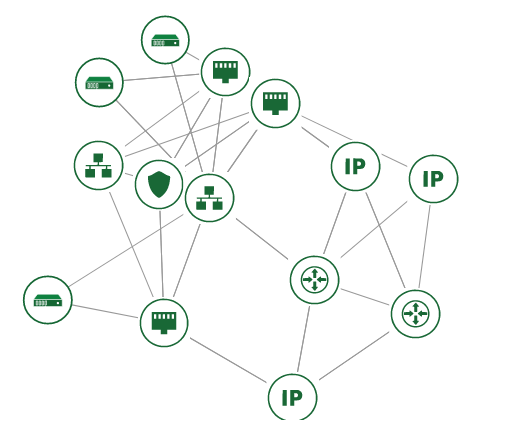
\includegraphics[width=\textwidth]{inc/images/DevOpsArchitecture.png}
    \caption{Server network architecture.}
    \label{fig:serverNet}
\end{figure}

The problem with using the stack for an automated process was that the team was unable to easily configure it together with \gls{jenkins} and \gls{docker}. The team knew that these services where often used together and with \gls{puppet} or \gls{chef} but were unable to find what tool was meant for what purpose. In the end the team used the \gls{hot} template tag to run a script for installing docker that would in turn setup \gls{jenkins} master and slave. Then \gls{jenkins} could be configured to handle pushes to \gls{git} repository and update the slaves. As the server configurations were incomplete, it was easier for each group member to host and test on their own local systems instead.

If the server configurations had been completed, the setup could have been used to ensure tests were run continuously and required for pull requests to be accepted. 

\section{Perspective on antlr}
\subsection{Overall reflection and experience}
Simple \Gls{antlr} workflow is explained in section \ref{sec:technicalBackEnd}. Each listener provides a context that represents a keyword within the file being parsed. The context is a sequential match of tokens. The number of tokens in a rule is the breadth of the context, whilst the depth of the context is the number of nested tokens before you reach a fragment that is a leaf node and a character sequence. The form of a token is an alternative rule that match the context.  

At the beginning of the project the group decided to parse some basic parts of the codebase to get familiar with \gls{antlr}, without thinking much about making it a proper system. This way the group was able to come up with a working prototype in the first week of development, but as the development progressed, the code would not scale due to a few tasks that required huge nested-if blocks to deal with the depth of the context. The problem with if statements is explained in sub section \ref{subsection:parsingJava}.

To retain the professionalism in the code, the group needed to find out a better way to use \gls{antlr} for code parsing. Through research and experiments the group came up with 3 solutions over time to structure the \gls{antlr} part of the codebase:
\begin{itemize}
    \item Stack
    \begin{itemize}
        \item In the \gls{antlr} repository it was recommended to use a stack like data structure to process the code \cite{github:stackAntlr}. Since \gls{antlr} parses the code sequentially, a stack could be used to store what is being parsed. This solved our problem with understanding the scope of a context by separating them. As \gls{antlr} runs on individual files, this approach was unable to identify scopes from different files. This was a problem with the C++ grammar as it sends include statements into a hidden channel. This meant that the group was unable to merge the different files into one project and connect structures and function calls declared in separate files.
    \end{itemize}

    \item Java Action
    \begin{itemize}
        \item Java Action was considered to help with contexts having large breadth and many forms where the context is known to have a wanted token. Actions would be for functionality to be added when entering or exiting a context. One could essentially say "When entering this scope; look for all instances of this token". It would return the wanted token no matter what sub-tree it was from, alleviating the need to check what form each nested context has. It would do this by setting an \gls{antlr} listener to call an Action that is overwritten when entering or exiting a scope.
    \end{itemize}

    \item \gls{antlr} visitors 
    \begin{itemize}
        \item The \gls{antlr} visitor were recommended to gain more control in traversing the parse-tree and are usually used if only sub-trees are required to be parsed. The project required many different components of the codebase to be parsed and listeners were therefor the best option for us, where it will go through every node in the parse tree. This way the listeners could sequentially parse every built-in keyword or user defined names from every line on the codebase.
    \end{itemize}
\end{itemize}

\subsection{Decreasing cyclomatic complexity in ANTLR}

\tikzset{
    vertex/.style = {
        circle,
        fill            = black,
        outer sep = 2pt,
        inner sep = 1pt,
    }
}
\begin{figure}[H]

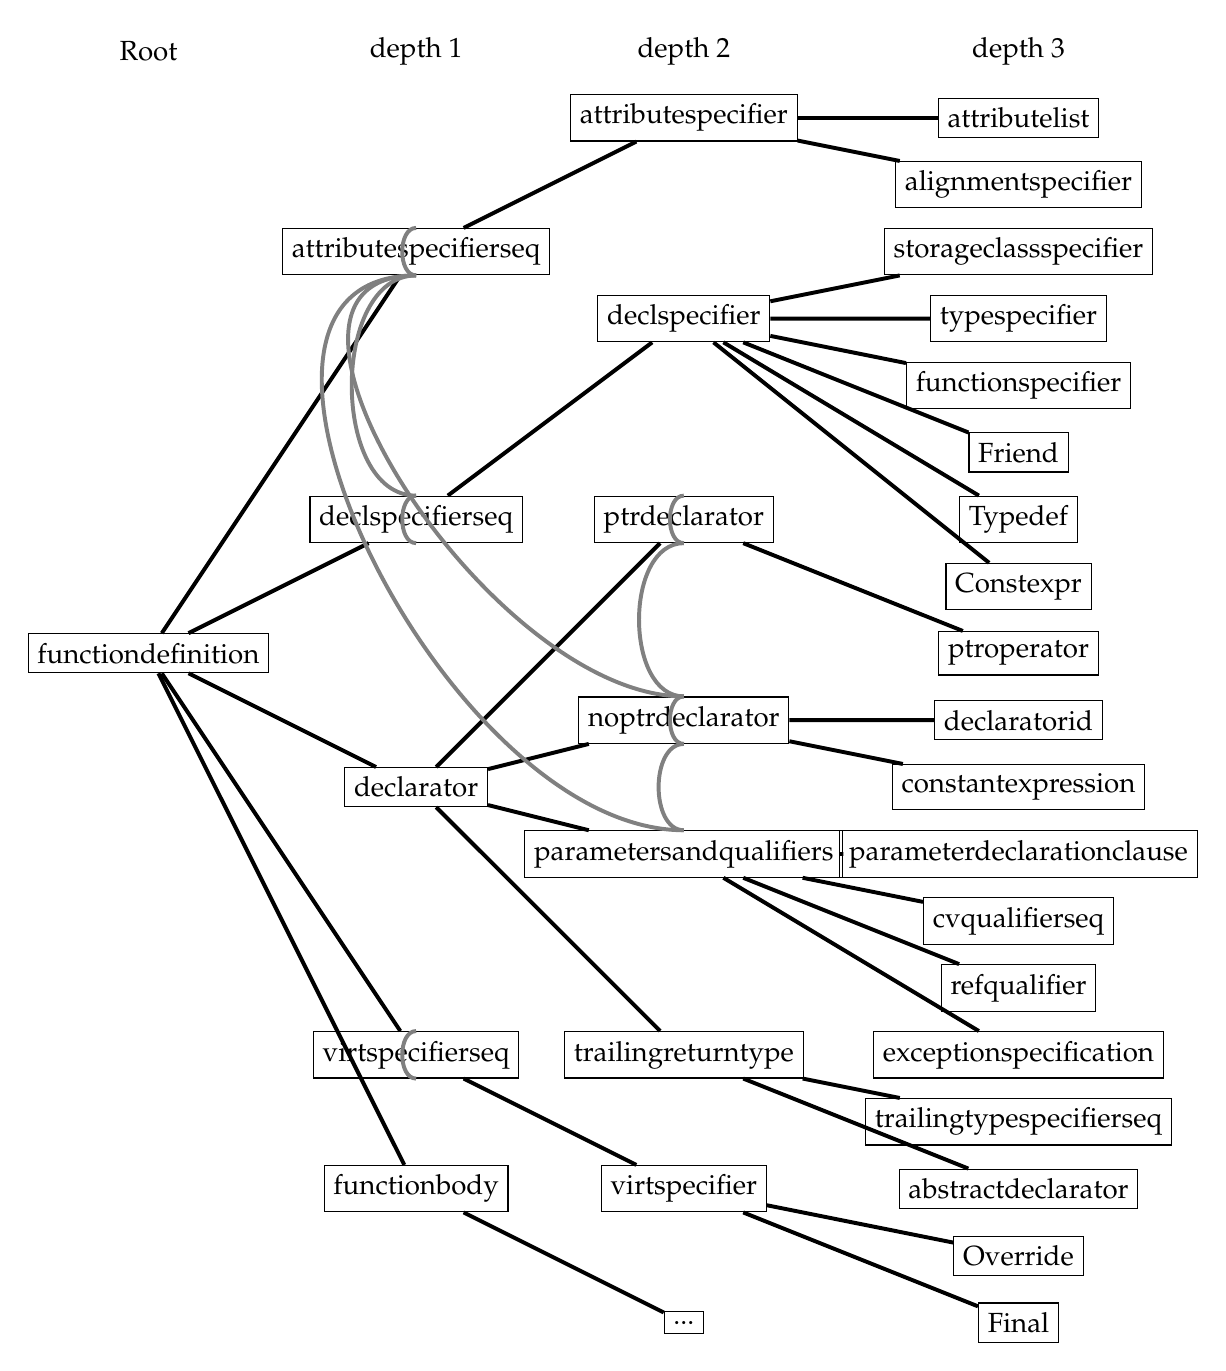
\begin{tikzpicture}[scale=0.85]
    % root
    \node at (0.0, 1.0) {Root};
    \node[draw] (funcDef) at (0.0, -8.0) {functiondefinition};
    
    %level1
    \node at (4, 1.0) {depth 1}; 
    \node[draw] (attribSeq) at (4, -2) {attributespecifierseq};
    \node[draw] (declSeq) at (4, -6.0) {declspecifierseq};
    \node[draw] (decl) at (4, -10.0) {declarator};
    \node[draw] (virtSeq) at (4, -14.0) {virtspecifierseq};
    \node[draw] (funcBody) at (4, -16.0) {functionbody};
    
    %root - level1
    \draw[line width=0.5mm,draw=black] (funcDef) to (attribSeq);
    \draw[line width=0.5mm,draw=black] (funcDef) to (declSeq);
    \draw[line width=0.5mm,draw=black] (funcDef) to (decl);
    \draw[line width=0.5mm,draw=black] (funcDef) to (virtSeq);
    \draw[line width=0.5mm,draw=black] (funcDef) to (funcBody);
    
    %level1 to exist
    \draw[line width=0.5mm,draw=gray] (attribSeq.south) to[in=180,out=180] (attribSeq.north);
    \draw[line width=0.5mm,draw=gray] (declSeq.north) to[in=180,out=180] (attribSeq.south);
    \draw[line width=0.5mm,draw=gray] (declSeq.south) to[in=180,out=180] (declSeq.north);
    \draw[line width=0.5mm,draw=gray] (virtSeq.south) to[in=180,out=180] (virtSeq.north);
    
    % level2
    \node at (8.0, 1.0) {depth 2};
    \node[draw] (attrib) at (8.0, -0.0) {attributespecifier};
    \node[draw] (declSpec) at (8.0, -3.0) {declspecifier};
    \node[draw] (ptrDecl) at (8.0, -6.0) {ptrdeclarator};
    \node[draw] (noptrDecl) at (8.0, -9.0) {noptrdeclarator};
    \node[draw] (param&qual) at (8.0, -11.0) {parametersandqualifiers};
    \node[draw] (trailReturn) at (8.0, -14.0) {trailingreturntype};
    \node[draw] (virtSpec) at (8.0, -16.0) {virtspecifier};
    \node[draw] (toMuch) at (8.0, -18.0) {...};
    
    %level1 - level2
    \draw[line width=0.5mm,draw=black] (attribSeq) to (attrib);
    \draw[line width=0.5mm,draw=black] (declSeq) to (declSpec);
    \draw[line width=0.5mm,draw=black] (decl) to (ptrDecl);
    \draw[line width=0.5mm,draw=black] (decl) to (noptrDecl);
    \draw[line width=0.5mm,draw=black] (decl) to (param&qual);
    \draw[line width=0.5mm,draw=black] (decl) to (trailReturn);
    \draw[line width=0.5mm,draw=black] (virtSeq) to (virtSpec);
    \draw[line width=0.5mm,draw=black] (funcBody) to (toMuch);
    
    %level2 to exist
    \draw[line width=0.5mm,draw=gray] (ptrDecl.south) to[in=180,out=180] (noptrDecl.north);
    \draw[line width=0.5mm,draw=gray] (ptrDecl.south) to[in=180,out=180] (ptrDecl.north);
    \draw[line width=0.5mm,draw=gray] (noptrDecl.north) to[in=180,out=180] (attribSeq.south);
    \draw[line width=0.5mm,draw=gray] (noptrDecl.south) to[in=180,out=180] (param&qual.north);
    \draw[line width=0.5mm,draw=gray] (noptrDecl.south) to[in=180,out=180] (noptrDecl.north);
    \draw[line width=0.5mm,draw=gray] (param&qual.north) to[in=180,out=180] (attribSeq.south);
    
    % level3
    \node at (13.0, 1.0) {depth 3};
    \node[draw] (attribList) at (13.0, -0.0) {attributelist};
    \node[draw] (alignmentspecifier) at (13.0, -1.0) {alignmentspecifier};
    \node[draw] (storageclassspecifier) at (13.0, -2.0) {storageclassspecifier};
    \node[draw] (typespecifier) at (13.0, -3.0) {typespecifier};
    \node[draw] (functionspecifier) at (13.0, -4.0) {functionspecifier};
    \node[draw] (Friend) at (13.0, -5.0) {Friend};
    \node[draw] (Typedef) at (13.0, -6.0) {Typedef};
    \node[draw] (Constexpr) at (13.0, -7.0) {Constexpr};
    \node[draw] (ptroperator) at (13.0, -8.0) {ptroperator};
    \node[draw] (declaratorid) at (13.0, -9.0) {declaratorid};
    \node[draw] (constantexpression) at (13.0, -10.0) {constantexpression};
    \node[draw] (parameterdeclarationclause) at (13.0, -11.0) {parameterdeclarationclause};
    \node[draw] (cvqualifierseq) at (13.0, -12.0) {cvqualifierseq};
    \node[draw] (refqualifier) at (13.0, -13.0) {refqualifier};
    \node[draw] (exceptionspecification) at (13.0, -14.0) {exceptionspecification};
    \node[draw] (trailingtypespecifierseq) at (13.0, -15.0) {trailingtypespecifierseq};
    \node[draw] (abstractdeclarator) at (13.0, -16.0) {abstractdeclarator};
    \node[draw] (Override) at (13.0, -17.0) {Override};
    \node[draw] (Final) at (13.0, -18.0) {Final};

    
    %level2 - level3
    \draw[line width=0.5mm,draw=black] (attrib) to (alignmentspecifier);
    \draw[line width=0.5mm,draw=black] (attrib) to (attribList);
    \draw[line width=0.5mm,draw=black] (declSpec) to (storageclassspecifier);
    \draw[line width=0.5mm,draw=black] (declSpec) to (typespecifier);
    \draw[line width=0.5mm,draw=black] (declSpec) to (functionspecifier);
    \draw[line width=0.5mm,draw=black] (declSpec) to (Friend);
    \draw[line width=0.5mm,draw=black] (declSpec) to (Typedef);
    \draw[line width=0.5mm,draw=black] (declSpec) to (Constexpr);
    \draw[line width=0.5mm,draw=black] (ptrDecl) to (ptroperator);
    \draw[line width=0.5mm,draw=black] (noptrDecl) to (declaratorid);
    \draw[line width=0.5mm,draw=black] (noptrDecl) to (constantexpression);
    \draw[line width=0.5mm,draw=black] (param&qual) to (parameterdeclarationclause);
    \draw[line width=0.5mm,draw=black] (param&qual) to (cvqualifierseq);
    \draw[line width=0.5mm,draw=black] (param&qual) to (refqualifier);
    \draw[line width=0.5mm,draw=black] (param&qual) to (exceptionspecification);
    \draw[line width=0.5mm,draw=black] (trailReturn) to (trailingtypespecifierseq);
    \draw[line width=0.5mm,draw=black] (trailReturn) to (abstractdeclarator);
    \draw[line width=0.5mm,draw=black] (virtSpec) to (Override);
    \draw[line width=0.5mm,draw=black] (virtSpec) to (Final);

    

\end{tikzpicture}

    \caption{CPP functiondefinition graph to depth 3.}
    \medskip
    \small
    Straight lines show that the, right-hand side is contained within the left side.
    Curved lines show that something defined earlier or at the same level is also within the rule.
    \label{CPPFunctionDefinition}
\end{figure}


When parsing function definition, it became clear that the depth of the context caused significant complexity as on each level the form of the context had to be checked. This required significantly nested if structures.

The team solved this problem partially using a stack of models. A model represents a structure in the codebase; for instance functions, classes, namespaces, etc. The model is added to the stack when it's scope is entered and removed after it has completed. This way the team was able to use specific listeners provided by \gls{antlr} to parse the specific fields for the model. 

With the stack, more listeners could be implemented without worrying that a listener would be called at the wrong time and the context be added in the wrong scope. Instead of parsing function definition in depth, one could implement the relevant listeners within the context and they would automatically add their data to their parent model where the parent model was function definition.
In figure \ref{CPPFunctionDefinition}, implementing functiondefinition to enter a function model and implementing typespecifier to add its type to the parent would mean function model would have this without explicitly checking declspecifierseq and declspecifier. 

Implementation of listeners in the object-oriented design created a lot of dependency relationships, which increased \gls{connacensemetrics} of the codebase. As figure \ref{CPPFunctionDefinition} shows every node in depth is dependent on its parent node, in most cases some nodes share the same parent node. This made it very difficult to figure out what listener could be executed next. The stack was still considered a good alternative as it removed a lot of \gls{cyclomaticcomplexity} and meant that more of the parsing burden was dealt with, by \gls{antlr}. 

Another solution for this could be using \gls{antlr} visitors, where visitors gives much more control on which token to visit. This way the team could exclude irrelevant sub-trees and only visit the information about a specific model. Due to time limitation, visitors were not experimented with, but this could be useful for future refactorings.

\subsection{Use of regex}
\newglossaryentry{regularExpression}{name={regular expression}, description={A sequence of characters that define a search pattern \cite{wiki:regex}}}
\newacronym{regex}{regex}{\Gls{regularExpression}}

Handling function calls was difficult as in Java and C++, the call can be called on an object and that object can in turn be called on any other object recursively. The grammar did not easily allow for the separation of these objects as the languages are very versatile with what an object might be. To bypass the difficulty of using \gls{antlr} for this purpose, the group decided to use \gls{regex}. The \gls{regex} was used to split the call on "." and "->" that delimited the different objects while other string operations were used to remove the body of some brackets. \Gls{regex} could not remove the content of the brackets correctly as they could in turn contain brackets and \gls{regex} can not handle \gls{recursion}. The content of brackets were removed to make it easier to identify the associated function. This approach would not scale in the long run and is likely to create problems. The problems that can arise, come from how this approach prevents \gls{antlr} from taking care of the recursive structure and niche aspects of the languages that the team has not considered. Removing the body also prevents the system from knowing what overloaded function is being called. Using the \gls{antlr} built-in features would be preferable in the long term, but would require significantly more work. 

The \Gls{regex} approach could also be used to parse function pointer assignments as this was a problem due to use of symbol "*" as a pointer and as a multiplication sign. This made it impossible for the team to differentiate between pointer assignments and multiplication expressions. A long term solution to this problem could be updating the grammar file with a rule for pointer assignments, but this was not done since it would require in-depth understanding of the grammar files. Function pointers were dropped due to time limitations.

\section{Perspective on REST and WebSocket}
As mentioned in sub section \ref{subsection:Go}, the \gls{rest} requirement of the project had to be relaxed. The addition of \glspl{websocket} was a necessary decision to take and integrate into the system. \Gls{websocket} are built-in to \gls{js}, a easy-to-use library for Go made it quick to set up and worked well for the purpose.

\Gls{websocket} is a different protocol that uses \gls{http} requests to request a \Gls{websocket} connection and then switches over to \Gls{websocket} protocol if server allows. This allows messages to be sent back and forth over 3 different channels, "open", "close" and "message". The "open" channel is for when the \Glspl{websocket} opens, "close" is for receiving shutdown message for the connection and "message" is for any information that needs to be sent. 

One solution to improve the \gls{rest} portion of the \gls{api} is to offer \Glspl{websocket}, along with a \gls{rest} \gls{api}, which will give next to no information about the parsing progress, but returns the same result.

The use of \gls{websocket} in Go led to very huge functions and this resulted in decreased readability of the endpoints. Huge functions were the side effect of error handling of \gls{websocket}. To improve readability the team could break the the functionality of the endpoint into multiple small functions.

One mitigation for the massive amount of error handling would be to use a concept called middleware. This is when you have code that is executed before or after any given code snippet for a specific reason. For example one could wrap a log-in functionality in middleware that would write to a log-file. This could log the users attempt and subsequent success or failure of the log-in. As well as logging, middleware could be used for prepping or extracting input to sensitive functions ensuring no \gls{taintPropogation} and injections, as well as handling errors.

\section{Perspective on Graphics systems}
\subsection{Overall reflection and experience}
Selection of a graphics system was relatively easy. The whole group had experience with OpenGL from the Graphics programming course \cite{course:graphics} and \gls{webgl} is closely related. Everyone already knew the details on how to draw in 3D, but since it was a new language the group didn't have much experience in, the group setup a workshop to familiarize with \Gls{js} and \gls{webgl}. The group also found THREE.js which is a well-known and well-used graphics framework in \Gls{js}. THREE.js handles \gls{webgl} automatically, was easy to use, contains ready made shapes called geometries and have a lot of support functionality like vector classes with built-in math. The group therefore decided to use THREE.js.

The project required to show information and interactable \gls{ui}, for this reason the group researched different \gls{ui} Libraries/frameworks found PixiJS, TWO.js, dat.GUI and ImGUI-js.

\subsection{Choice of graphics framework}
Using THREE.js meant that the graphics handling was not a problem, but there were still a problem with using the parsed codebase to create the 3D representation. This was handled in \Gls{js}, although later it seemed like parts of it could be handled by the \gls{backend} and allow for an improved web \gls{api} and better caching opportunities. 

\subsection{Choice of UI framework}
The group thought about creating a custom \gls{ui} system using PixiJS or TWO.js instead of using other existing libraries. This seemed like a lot of management and adjustment work, considering it would only be used for the visualization. 

dat.GUI is a pure \Gls{js} and HTML \gls{ui} Library. Although it seems easy to use and could possibly work, it seemed too simple from available \href{https://workshop.chromeexperiments.com/examples/gui/#1--Basic-Usage}{examples}. This would require large amounts of configuration code and would stretch the library's capabilities, which wasn't really desired. Only scenarios where "dat.GUI" would fit well is for a settings or configurations drop-down menu.

ImGUI-js is a 3rd party library and must work in unison with ImGUI, but the difference from TWO.js and PixiJS is that ImGUI-js wrappes ImGUI, so in-effect they're one library and this made it very difficult to integrate, therefore lot of time went into making it work properly, but the group did not have to get two libraries to work at the same time. Another benefit of ImGUI is that the \gls{ui}-elements exists inside windows which are by default movable and scalable. This results into a very customizable \gls{ui} layout out of the box if this is wanted.

\subsection{Choice of Application Lifecycle Framework}
\newacronym{alf}{ALF}{Application Lifecycle Framework}

The group considered to use framework for \gls{frontend} development because the use of framework is often recommended, especially when using \Gls{js} due to the way it handles scopes. The supervisor recommended multiple frameworks such as POLYMER.js, VUE.js, AngularJS and REACT.js. The project is a web-based application which has only two HTML pages and most of the \gls{frontend} deals with graphics.

Considering this the team later realized that there was no need for it. Most \glspl{alf} are not designed for graphics and therefore did not fit well with this application. It could restrict and require time to learn without giving any significant benefits.

\subsection{Use of Force Directed Graph library}
There are a multitude of libraries out there that handles \gls{fdg} quite good like \href{https://www.npmjs.com/package/3d-force-graph}{3d-force-graph} and \href{http://getspringy.com/}{Springy.js}, but none of these libraries allowed for individual link strengths. They only have a single global setting for all attractive links, and the reason this was wanted was due to the different data structures being more or less attracted to other certain data structures. Therefore it was decided to not not integrate any \gls{fdg} library. 

\subsection{Graphics system refactoring}
The 3D representation was changed multiple times but not fully refactored so it still contains code that should have been deprecated, removed or changed to fit the rest of the system. Some of these changes were made late in the project when time-constraints were causing problems. The time-constrains meant that proper refactoring would not improve the velocity of the team and were therefore not prioritized.

\section{Perspective on FDG}
\subsection{Overall reflection and experience}

The codebase visualization had to be intuitive and able to handle both large and small datasets without any manual adjustment by the user or administrator. A \gls{fdg} seemed like a natural choice for automatically adjust the layout based on the scale and composition of the codebase. It also seemed natural to use the scoping in object oriented programming to hide or reveal details based on what the user was looking at.

As this was the first time the group had used \gls{fdg}, it was a surprise how flexible the literature was about the implementation specification. The literature helped establish a few terms:

\begin{itemize}
    \item Node - A representation of codebase structure with positional data and metadata requiered by \gls{fdg} to update position.
    \item Energy - relating to the total energy in the system and what the \gls{fdg}'s goal was to minimize.
    \item Attractiveness - metadata of node relating to how much energy is required to keep it apart from one other node.
    \item Repulsiveness - metadata of node relating to how much energy is required to keep it close to one other node.
    \item Links - metadata of node, a map of all repulsive and attractive forces to all other nodes.
    \item Gravity - A global force affecting all nodes, pulling them towards a defined center.
\end{itemize}

\subsection{Detailed experience on refactoring of FDG}
The \gls{fdg} is probably the part in the program that caused the most problem when trying to expand on it and refactor it.
It started off as a prototype with limitations:
\begin{itemize}
    \item Assumed no nested structures as output.
    \item Assumed a global center that all structures should gravitate towards to keep the graph centered.
    \item Assumed an initial repulsion from one structure to another, that's not related and of equal strength.
    \item Assumed the repulsive forces was negative by the algorithm.
    \item Assumed all repulsive forces were set as -1 by the parsing.
    \item Assumed a connection or attraction from structures based on nested structures in input.
\end{itemize}

The \gls{fdg} used Inverse-square-law to calculate force based on repulsiveness and Hooke's law to calculate a force from attractiveness. All the nodes were parsed from the initial nested codebase structure in pre-order and stored in a single array within the \gls{fdg} object.
The initial structure allowed for relatively simple parsing and well understood and fairly versatile structures. Initially it was desirable for nodes to contain minimal information and only the information required by \gls{fdg}. This would improve the object oriented model and minimize the amount of data being passed around. The desire to keep nodes minimal was lessened when the group looked into \gls{js} as a "Share by Calling" language. 

When it came to changing \gls{fdg} to allow for nested structures as output, it soon became clear that large portions would have to be changed. The wish was to have a system that would be streamlined and versatile. This meant to change array containing all the nodes into a generic tree that more closely represented both the input and output data. It was required to change the single array approach as allowing for nested output, which meant the \gls{fdg} would have to run on each nested part separately. Changing the array proved complicated, as links were added while parsing the input and used the index in the array to identify the other node, with a tree, the index would have to be calculated and kept constant. It was thought that keeping the index constant could only be done by parsing the input level-order or pre-order, and this would not allow for nested output as the size of each node was dependent on its children. Therefore the parsing was done post-order and contained a local index that could be used to calculate the global index in the tree when connected to the root. This result is described in sub section \ref{subsubsec:recuriviryOfNode}. This assumption turned out to be wrong, and giving the nodes a global index when building the tree would have been beneficial.

The local to global calculations caused a lot of confusion and significantly increased complexity. The new system had the same cyclomatic complexity as before, keeping conditionals essentially the same, but increased the use of complicated \gls{recursion} and had a high connacance with the removed array through the global index.

Although there were made mistakes during the refactoring and it increased the complexity, it was still beneficial. Benefits of using the tree structure were evident, as the group could run \gls{fdg} on each node separately from the world origin and input this to the \gls{scenegraph} to handle offsets and potential navigation. From parsing in the \gls{backend} to the visualization in \gls{frontend}, the core data is always handled as a tree structure. This means there is a high level of consistency throughout the system but also an implicit connacance that means if the structure is changed in one part of the system then all other parts will also have to be changed.

\section{"sloccount" vs "Kloc" vs "wc -l"}
One of the simplest complexity metrics to add was \gls{loc} and was added as a first, simple metric. Sloccount, \gls{kloc} and wc are tools that can get the \gls{loc}. wc was chosen. 
wc is a linux command line tool to read words, newlines and bytes and prints out the result to standard output channel. wc is language independent meaning it can take any language file as an argument. It can also read only the specified lines within the files by giving the "-l" flag when executing. This worked well for our purpose and therefore used to fetch the implementation from source code files. The other alternatives were considered because wc would not be able to distinguish between comments, code or empty lines, but the other alternatives had the same limitations or would not support enough languages for our purpose. 

\section{Platform for the product}
The reason of choosing web as the platform for the the system was for it to be cross-platform and so that any user could easily access the system from anywhere. Also the team did not have much experience in the web-technology therefore it was a good opportunity to implement the system as web-service.
\gls{js} is the technology the team didn't not have much experience with and become a problem to scale as responsibilities of \gls{frontend} increased over time.

\section{Post-phoning/removing userstory allowing user to submit lexer files}
There was an idea early on that the user would be able to input a lexer file for any language and be able to use it to visualize projects written with-in that language. It became clear very quickly the more the team worked with \gls{antlr} that this feature was not going to be integrated. The listener files are generated based on the grammar file and are language specific, which means one would have to implement each listener independently for each language for the system to be able to parse that language. So to integrate the submitted lexer files, the application have to either inject the new code in during runtime which is far beyond the project scope. It was decided to drop this functionality due to the shear size of this feature, which on its own can be counted as a bachelor if not even more.
\chapter{Conclusion}
\label{chap:conclusion}
\section{Result}
The result is a prototype capable of handling Java and C++ and gives a decent indication of simple code quality and complexity. It visualizes data structures in the 3D environment in a clear and intuitive manner, although contains some duplicate data. The product owner requested a system that could be used to identify good or bad libraries, which the system gave a minimal but sufficient indication of through the visualization. It provides a good bedrock for future development, graduation projects or master thesis.

\section{Future Work}
\label{sec:future}
The project could be continued in a master thesis as a research or personal project where some of the following items could be integrated or improved upon:

\begin{itemize}
    \item Integrate AI to do language recognition.
    \item Integrate virtual reality for visualization.
    \item Extend a \gls{rest} \gls{api} to be more independent from systems \gls{gui}, but also fetch desired parts of parsed code through \gls{rest}.
    \item Spacing as sizing algorithm could be implemented in a proper manner insuring children do not escape their parents nor would collide with siblings.
    \item File tree structure could be implemented and visualized within the window.
    \item \gls{frontend} could be refactored to a properly segmented and professional system.
    \item The camera controls could be improved to become more intuitive
    \item Adding user settings/account capabilities for remembering locale, submitted repositories, custom styles and saving the world state properties to continue the inspection from the same point or preparation.
    \item Integrate  GraphQL to fetch specific scopes from the parsed code, to save on parsing and loading resources.
\end{itemize}

\section{Evaluation of group work}
Throughout the development, all team members worked well and tried their best to create the best product possible. Despite problematic tasks and new technologies to learn, the group progressed and overcame most hinders.

\section{Ending}
All in all the group is happy about the work done in this project and the knowledge acquired throughout. The group is happy about the quality and consider the project well made, although a few parts could have been done better.


\bibliographystyle{ntnuthesis/ntnubachelorthesis}
\bibliography{inc/BibTex}

\appendix %after this line all chapters will have letters instead of numbers
\chapter{Initial Project Description}   \label{appendix:initialProjectDescription}
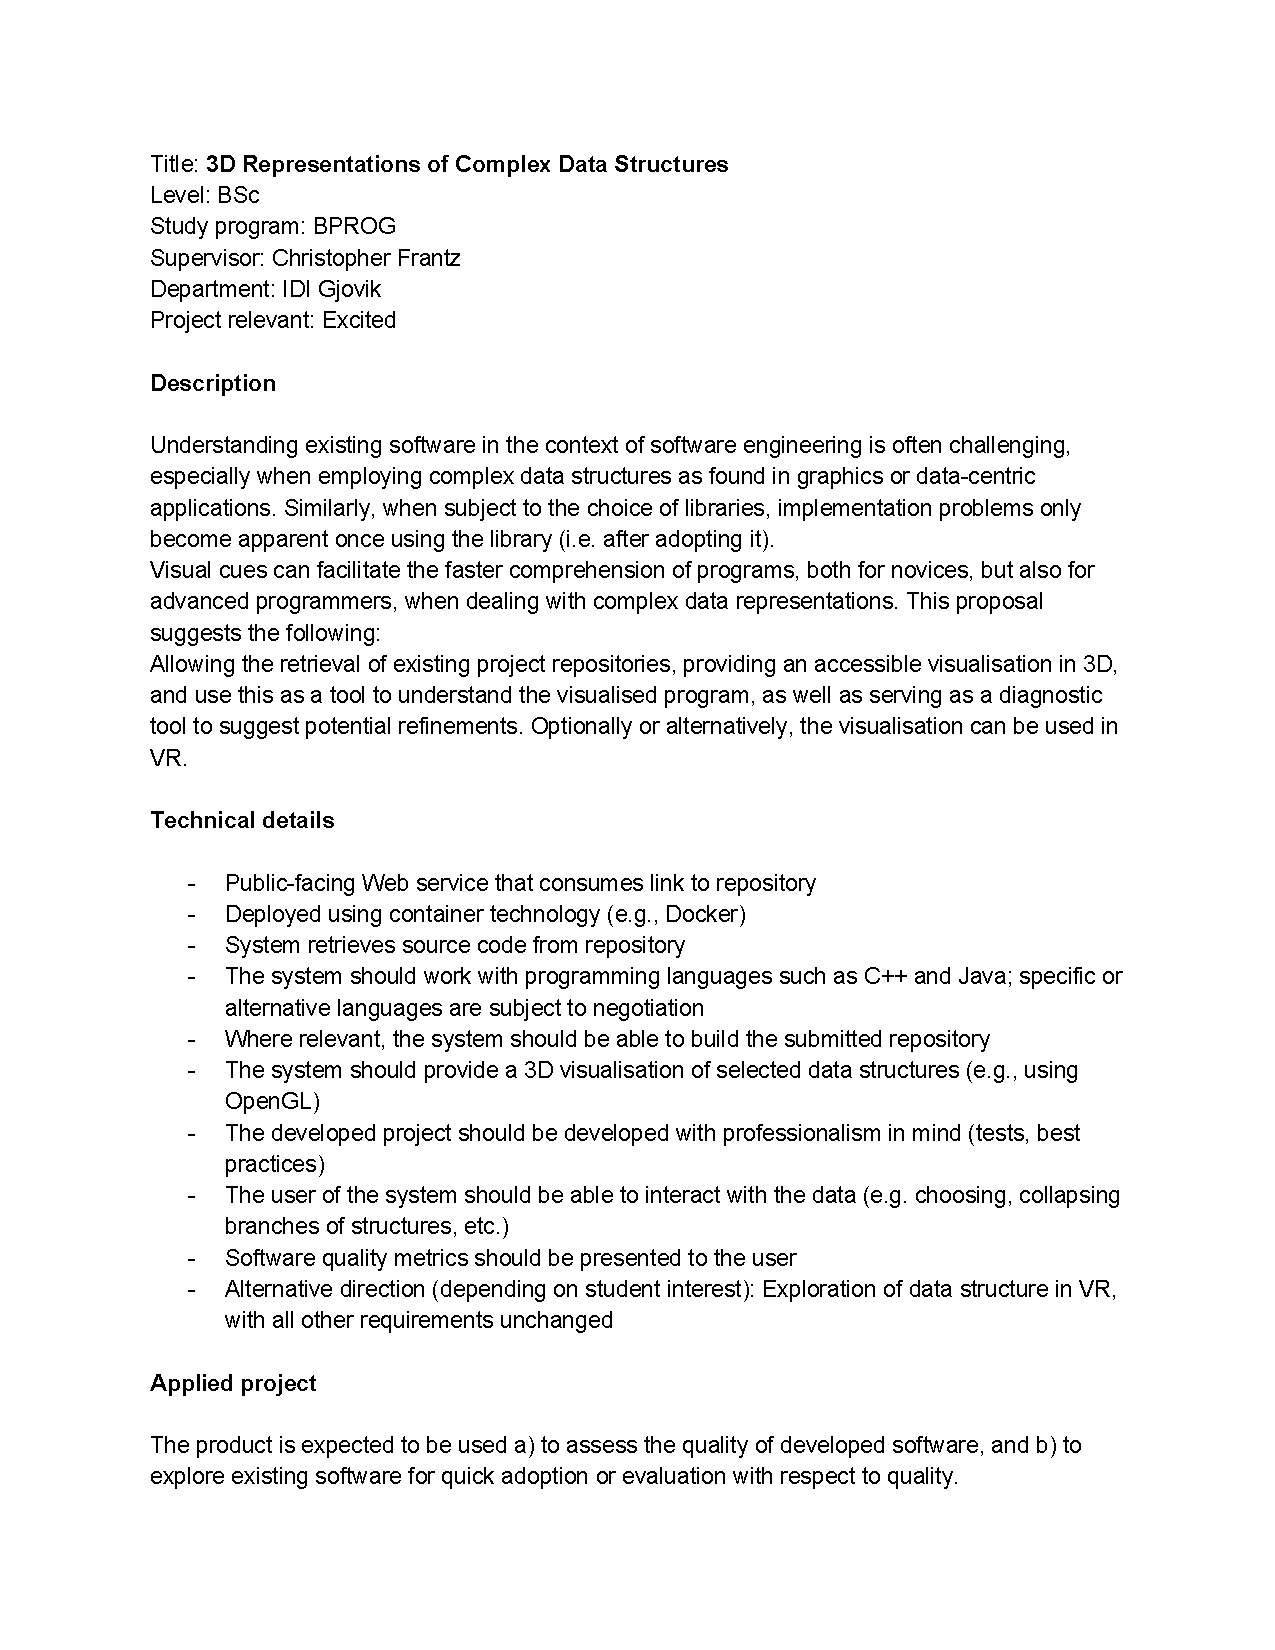
\includepdf[pages={-}]{inc/generalAppendix/3DRepresentationofComplexDataStructures.pdf}
\chapter{Project Plan}
\label{app:projectPlan}

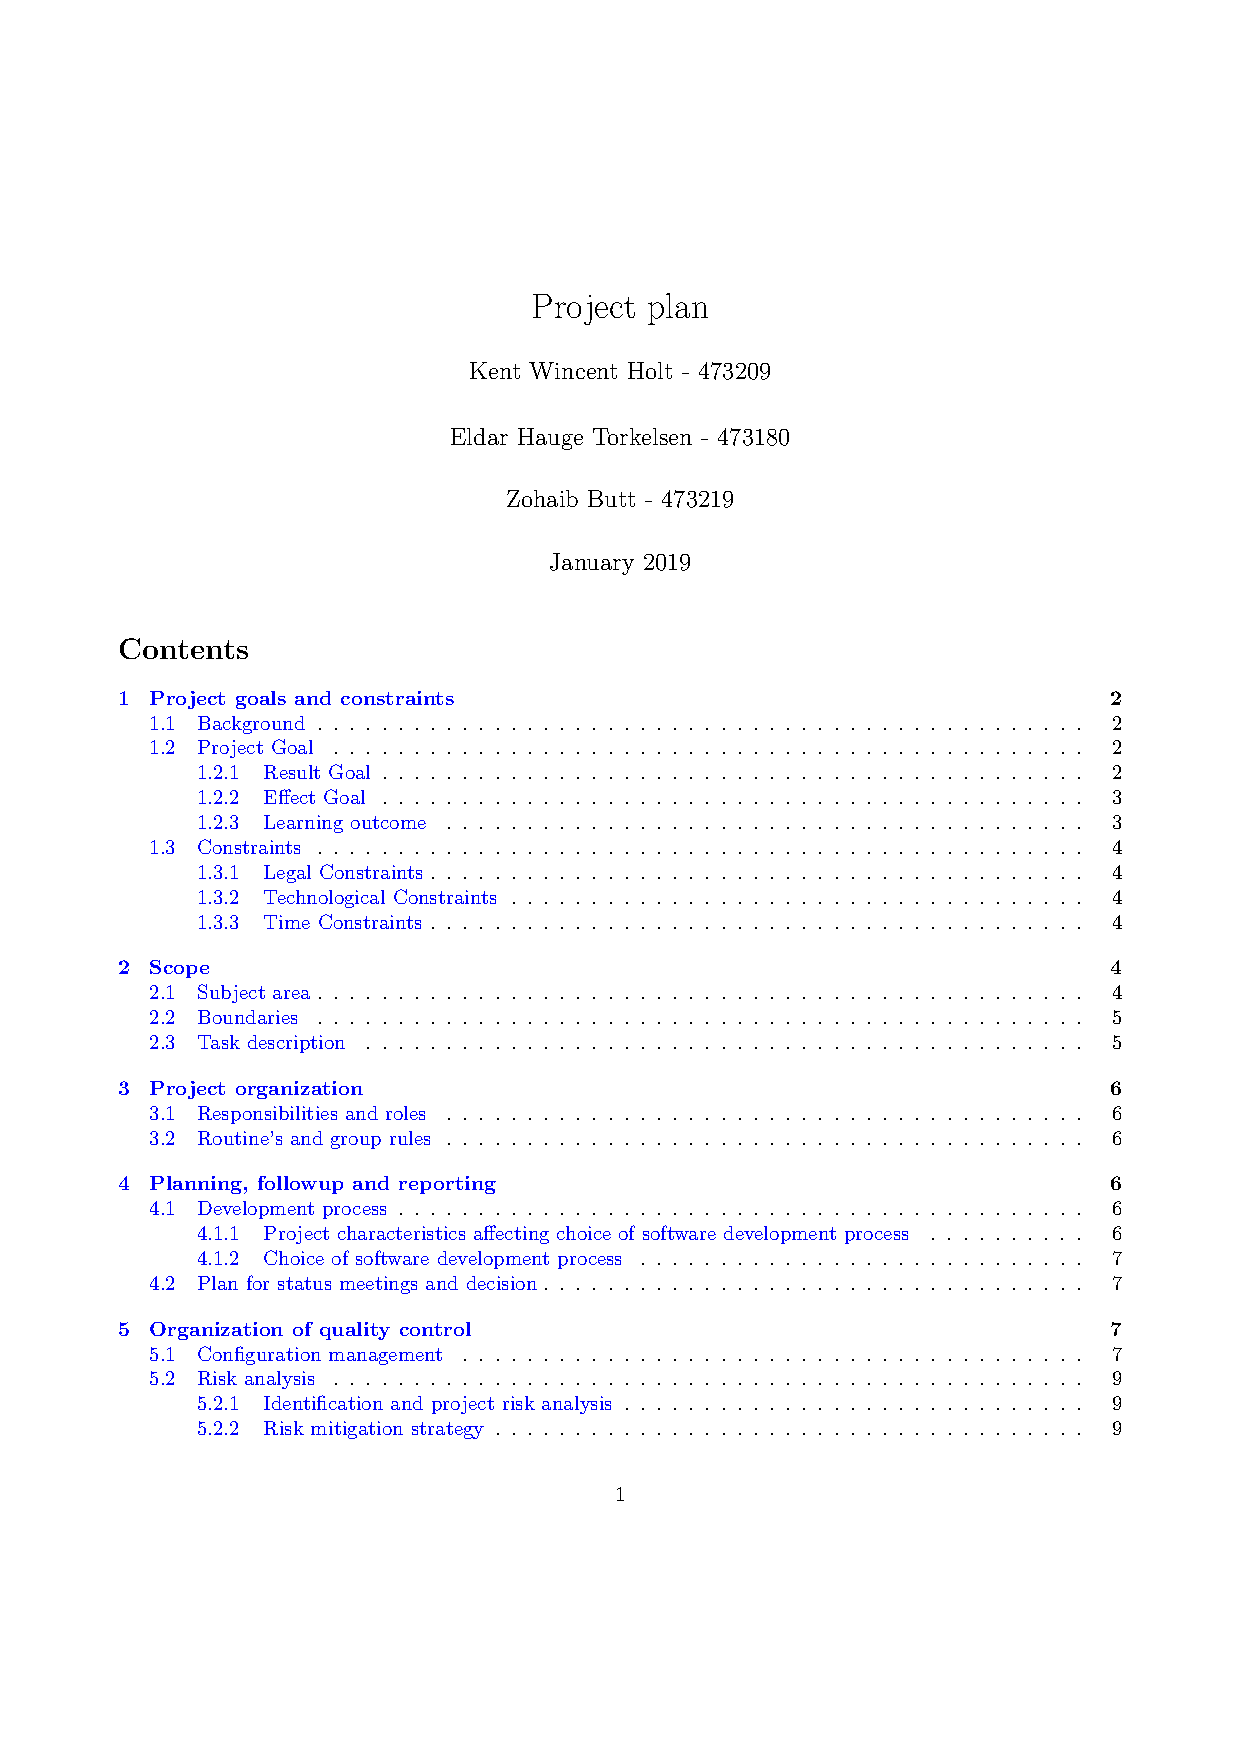
\includepdf[pages={-}]{inc/generalAppendix/Bachelor_Thesis.pdf}

\chapter{Project Agreement}
\label{app:agreement}

\includepdf[pages={-}]{inc/NTNUProsjektavtale.pdf}


%\input{inc/gantt}
\chapter{User study}
\label{app:userStudies}
\section*{Norwegian}

\begin{itemize}
    \item \textbf{Introduksjon} - "Hei, Jeg representerer en bachelor gruppe some har jobbet med å representere codebaser fra git repositories."
    \item \textbf{Be de lese kode eksemple} - "Vensligst les denne kode snutten i c++. Hvis du har noen spørsmål, gjerne spør. Det er ikke deg vi tester, vi tester systemet."
    \item \textbf{Be de tegne strukturen} - "Vennligst tegn hvordan du ville ha visualisert datastrukturen og forklar tankegangen din."
    \item \textbf{Be de sende inn en Git URL til systemet} - "Dette er hjemme siden for systemet. Kan du prøve å representere følgende Git repo: https://github.com/zohaib194/COVI\_test01.git"
    \item \textbf{Få dem til å hente implemntasjon av main() funksjon} - "Er det mulig om du kan finne kilde koden i main funksjonen innen dette systemet?"
\end{itemize}

\section*{English}

\begin{itemize}
    \item \textbf{Introduction} - "Hi, I represent a group working on a graduate project, trying to represent code-bases from git repositories."
    \item \textbf{Have them read the code-example} - "Please read this c++ example. If you have any questions don't hesitate to ask, as we are not testing you, but the system."
    \item \textbf{Have them draw the structure} - "Please draw how you would represent the code-base and also explain why you represent the code like you do."
    \item \textbf{Have them submit the git URL} - "This is the home page of the system. Could you try to use it to get a representation of the code at the git repository: https://github.com/zohaib194/COVI\_test01.git" 
    \item \textbf{Have them get the main() implementation} - "Is it possible for you to view the source code of the main function within the system?"
\end{itemize}
\section*{Questionair}
\label{sec:questionair}
\begin{itemize}
    \item \textbf{How confident are you with the object-oriented paradigm?} - From 1 to 5.
    \item \textbf{How confident are you with C++?} - From 1 to 5.
    \item \textbf{How useful is the information on the homepage?} - From 1 to 5.
    \item \textbf{How intuitive is it to navigate within the visualization?} - From 1 to 5.
    \item \textbf{How easy is it to find the implementation / source code for a function?} - From 1 to 5.
    \item \textbf{How intuitive is the visualization?} - Long text answer.
    \item \textbf{Do the shapes and color differentiate the various data structures clearly?}  - From 1 to 5.
    \item \textbf{Do think a customizable GUI would improve the usability?} - From 1 to 5.
    \item \textbf{Suggestions for customizable GUI (if any)} - Long text answer
    \item \textbf{How likely is it that you will have a use for such a system in the future?} - From 1 to 5.
    \item \textbf{Any features you feel are missing?}  - Long text answer
    \item \textbf{Any additional feedback on the entire project.}  - Long text answer
\end{itemize}
\section{Participation notes 1}
Participant: Professional.

\begin{itemize}
    \item \textbf{Have them read the code-example} -  Participant did not have any problem reading the code.
    \item \textbf{Have them draw the structure} - The participant started with drawing the execution flow of the main function using a circle and called it "start", then added two boxes and said this was the two functions side the "World" namespace and drew an arrow from main to the first function main called, then from that function to the second function. Then from the second function to a circle named "end". After this it was mentioned to visualize the "World" namespace, the participant drew a box surrounding the two functions within it and called it "World" at first but then shifted this to be the "std" namespace and draw another namespace box around the whole visualization and called it "World".
    \item \textbf{Have them submit the git URL} - URL submission went without problem and seemed to be intuitive although the participant used the cached input on the URL field and did not type it fully.
    \item \textbf{Have them get the main() implementation} - Participant was able to find implementation of main. Participant wasn't able to find the implementation of the other functions.
    \item \textbf{Participant visualization} 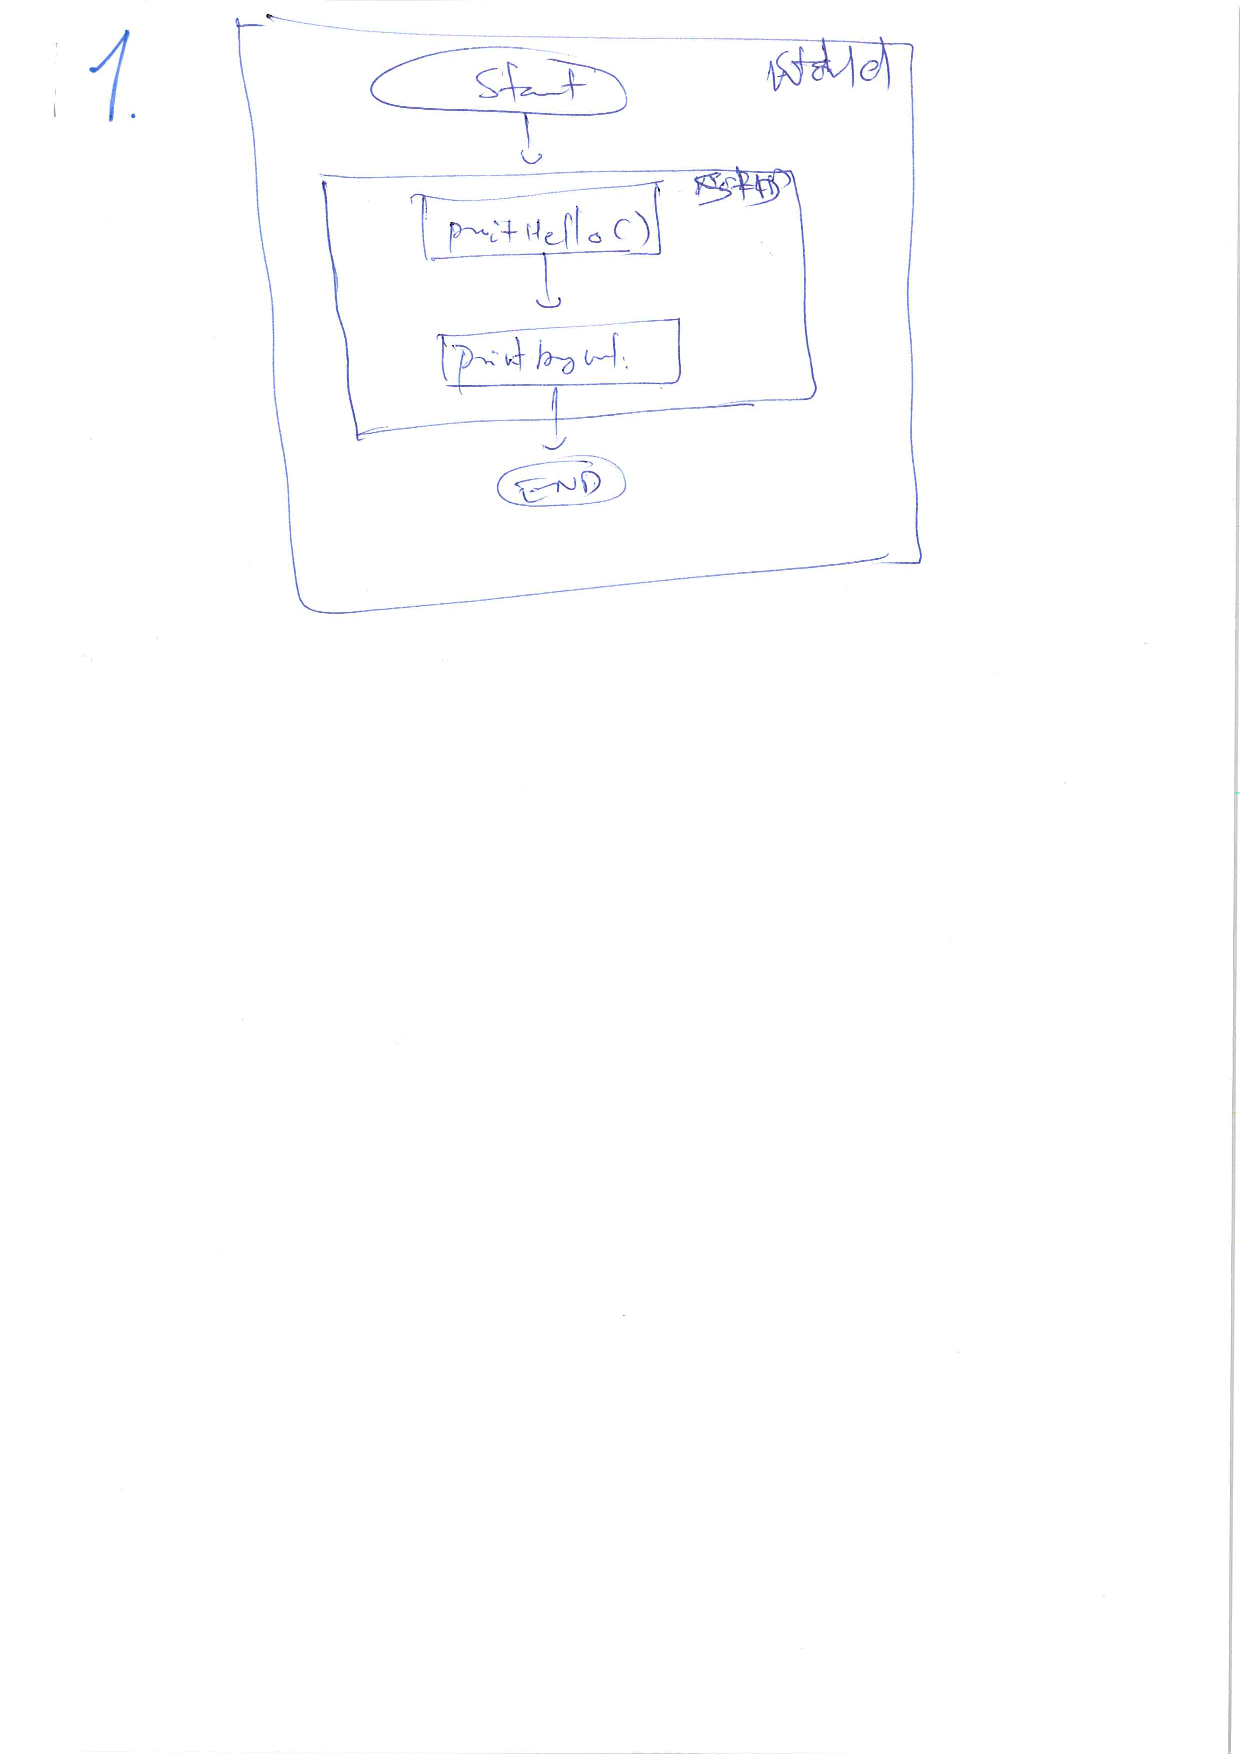
\includepdf[pages={1}]{inc/generalAppendix/userStudies/participantsVisualization.pdf}
\end{itemize}{}

\section{Participation notes 2}
Participant: Student

\begin{itemize}
    \item \textbf{Have them read the code-example} - Participant did not have any problem reading the code.
    \item \textbf{Have them draw the structure} - Participant separated the two called functions into each their circle and added names to each of them. Participant then represented main as a square and drew arrows from main to each function and explained that they were function calls.
    \item \textbf{Have them submit the git URL} - Participant wrote into the git repository field and submitted without problem. Afterwards, the participant used mouse to navigate successfully.
    \item \textbf{Have them get the main() implementation} - Participant was able to find implementation of both main and other functions.
    \item \textbf{Participant visualization} \includepdf[pages={4}]{inc/generalAppendix/userStudies/participantsVisualization.pdf}
\end{itemize}
\section{Participation notes 3}
Participant: Student

\begin{itemize}
    \item \textbf{Have them read the code-example} - Participant did not have any problem reading the code.
    \item \textbf{Have them draw the structure} - Initially the participant seemed confused by the question, but started drawing to explain the code structure. User represented the code as a conveyor belt with packages on top. the packages were the two functions being called by main. 
    \item \textbf{Have them submit the git URL} - User wrote in the URL and submitted. Participant then used the mouse for navigation and note that lines represent function calls and that the representation makes somewhat sense. 
    \item \textbf{Have them get the main() implementation} - Participant mentions that the participant does not know at all if task is possible, but continues for a while before clicking the function. Despite the implementation being shows, the participant is unaware and answers that participant does not know.
    \item \textbf{Participant visualization} \includepdf[pages={6}]{inc/generalAppendix/userStudies/participantsVisualization.pdf}
\end{itemize}
\section{Participation notes 4}
Participant: Teacher

\begin{itemize}
    \item \textbf{Have them read the code-example} - Participant mentions that participant has very limited experience with C++ in particular. 
    \item \textbf{Have them draw the structure} - 
    \item \textbf{} - User explains that there is a main procedure and two under-procedures called by main. Namespace is a concept that the user has little experience with, but draws it as a dotted line around the two sub procedures. Participant then mentions the control flow going from main to the two sub procedures. 
    \item \textbf{Have them submit the git URL} - User reads the description before clicking the submit button without content repository field. User then mentions that nothing happen when clicking submit and is unable to continue without guidance.
    \item \textbf{Have them get the main() implementation} - Participant tries to use the top bar menu and does not try the navigation within the expected time. When main is visible, the user immediately clicks it to get implementation.
    \item \textbf{Participant visualization} \includepdf[pages={7}]{inc/generalAppendix/userStudies/participantsVisualization.pdf}
\end{itemize}
\section{Participation notes 5}
Participant: Student.

\begin{itemize}
    \item \textbf{Have them read the code-example} - Participant did not have any problem reading the code.
    \item \textbf{Have them draw the structure} - The participant started with drawing a box and called it "namespace". Within this box, two lines where written inside and was said to be the functions inside the "World" namespace. Then the participant wrote "Main" and drew two half circles on either side and said that this represented the main function. Inside of the half circles 2 lines where written as calls to the first, then second function and then a "return 0" line.
    \item \textbf{Have them submit the git URL} - URL submission went without problem and seemed to be intuitive although the participant used the cached input on the URL field and did not type it fully.
    \item \textbf{Have them get the main() implementation} - Participant was able to find implementation of main. Participant wasn't able to find the implementation of the other functions.
    \item \textbf{Participant visualization} \includepdf[pages={2}]{inc/generalAppendix/userStudies/participantsVisualization.pdf}
\end{itemize}
\section{Participation notes 6}
Participant: Student

\begin{itemize}
    \item \textbf*{Have them read the code-example} - Participant did not have any problem reading the code.
    \item \textbf*{Have them draw the structure} - The participant focused on the output of the code. Visualized the "cout" as speach bubles and the code base as a blueprint.
    \item \textbf*{Have them submit the git URL} - URL submission went without any problem and camera controlls seemed to be intuitive.
    \item \textbf*{Have them get the main() implementation} - Fetching implementation of main function worked without any problem. Participant also used the code on paper and visualization for navigation of calls. Other functions implementation wasn't intuitive to fetch.
    \item \textbf*{Participant visualization} \includepdf[pages={5}]{inc/generalAppendix/userStudies/participantsVisualization.pdf}
\end{itemize}
\section{Participation notes 7}
Participant: Professional

\begin{itemize}
    \item \textbf{Have them read the code-example} - Participant has no issue understanding the code. 
    \item \textbf{Have them draw the structure} - User mentions taking inspiration from DFD or Data Flow Diagram when writing. The participant then followed up by drawing the namespace as an oval and the inner functions as circles with square, triangle and a number in each. The user mentioned doing so to idenify the different functions. Under the drawing, a pipeline was drawn a square connected to the first function and then to the second function and then on to a circle. The connections were drawn as arrows. 
    \item \textbf{Have them submit the git URL} - Participant changed  the content of the repository form and used mouse to navigate once the visualization appeared. The user then mentioned that it was a good way to visualize the code.
    \item \textbf{Have them get the main() implementation} - Participant immediately clicked on the function and sees the implementation of main, but struggled to get the implementation of the other functions. 
    \item \textbf{Participant visualization} \includepdf[pages={8}]{inc/generalAppendix/userStudies/participantsVisualization.pdf}
\end{itemize}
\section{Participation notes 8}
Participant: Student.

\begin{itemize}
    \item \textbf{Have them read the code-example} - Participant did not have any problem reading the code.
    \item \textbf{Have them draw the structure} - The participant drew three Boxes the title "Main", "Hello world" and "Bye world". Within box "Hello world" and "Bye world" a general form of the implementation of the individual functions was written. In side the main box, the prticipant added two dots one above the other and drew two arrows, one from the top dot to the "Hello world" box and a second from the "Bye world" box and said this was said to represent the function calls in main. After this a line was added underneath the two dots within the box called "Main" which said "return" which was mentioned to be the return of the main function.
    \item \textbf{Have them submit the git URL} - URL submission went without problem and seemed to be intuitive.
    \item \textbf{Have them get the main() implementation} - Participant wasn't able to find implementation of both main and the other functions.
    \item \textbf{Addition notations} - Clicked the list of submitted repositories. The participants was able to scroll in/out. Participants had no problem with the camera controls.
    \item \textbf{Participant visualization} \includepdf[pages={3}]{inc/generalAppendix/userStudies/participantsVisualization.pdf}
\end{itemize}
\section{Participation notes 9}
Participant: Student

\begin{itemize}
    \item \textbf{Have them read the code-example} - The user mentions being confused by the task.
    \item \textbf{Have them draw the structure} - The participant explains drawing the namespace as a separate thing with two functions in it. The two functions print and are called by main which is outside the namespace.
    \item \textbf{Have them submit the git URL} - User writes into the git repository field and reads the description before clicking the submit button. The participant then mentions seeing a line before navigating using the mouse. 
    \item \textbf{Have them get the main() implementation} - The user clicks the main function and says it is possible to view the implementation, but seem confused when trying to get the other functions. First saying it is not possible before changing opinion. 
    \item \textbf{Participant visualization} \includepdf[pages={9}]{inc/generalAppendix/userStudies/participantsVisualization.pdf}
\end{itemize}
\chapter{Design}
\section{Initial visualization concept}
\begin{figure}[H]
    \centering
    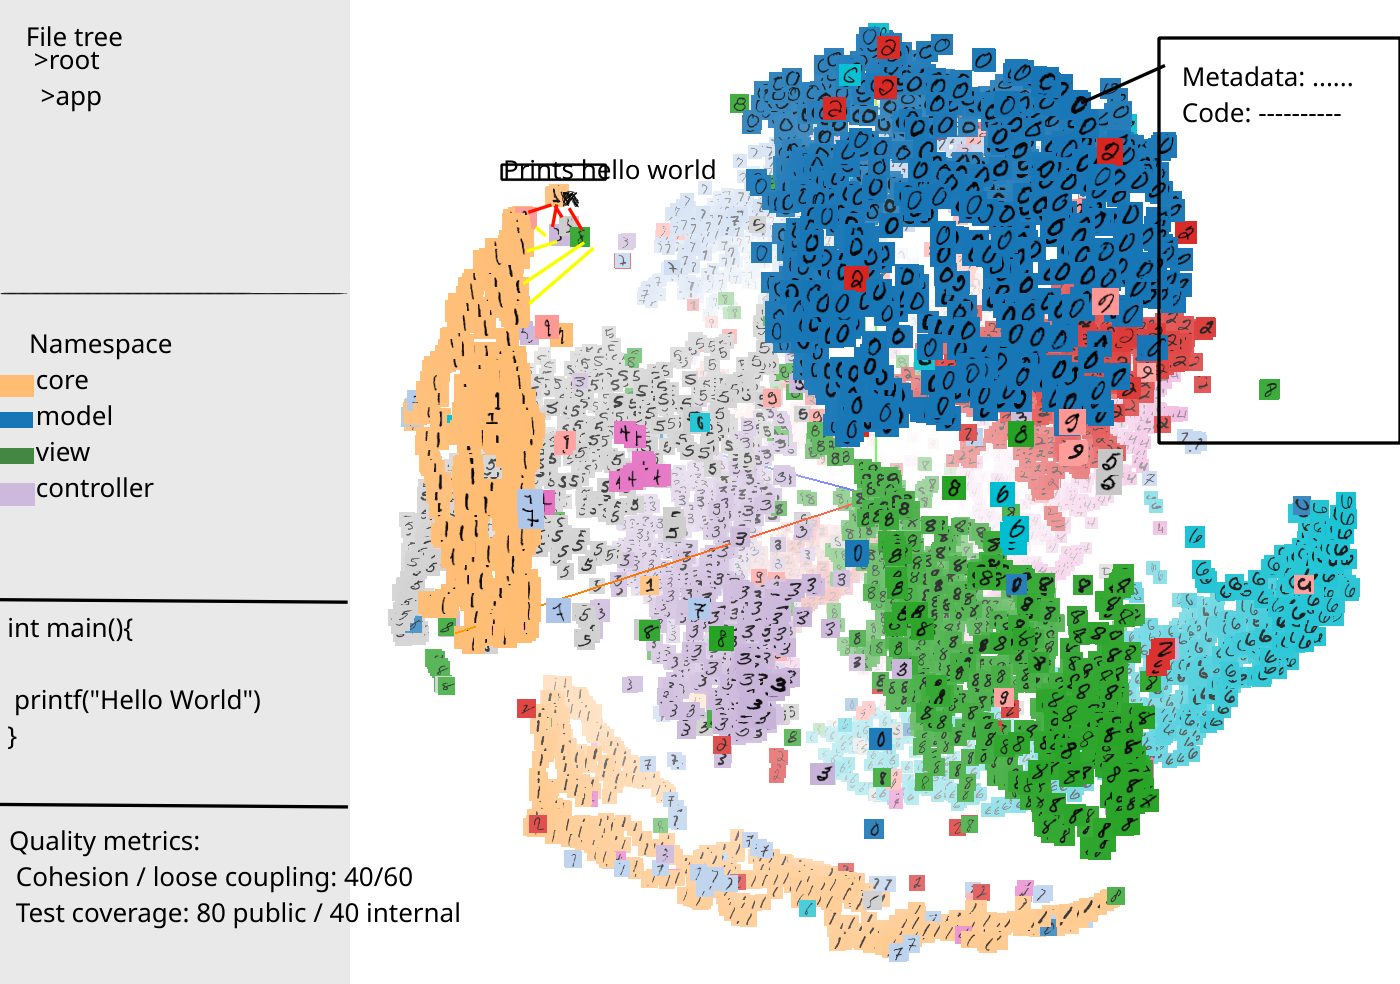
\includegraphics[width=\textwidth]{inc/images/tensorVisualization.png}
    \caption{Initial UI concept.}
    \label{fig:uiConcept}
\end{figure} \label{app:initialConcept}
\section{Logo concepts}
\begin{figure}[H]
    \centering
    
\includegraphics[width=\textwidth]{inc/images/CodeVis3D_logos.png}
    \caption{Logo for large and small format.}
    \label{fig:logos}
\end{figure}
\chapter{Jira exported decision log}    \label{appendix:decisionLog}
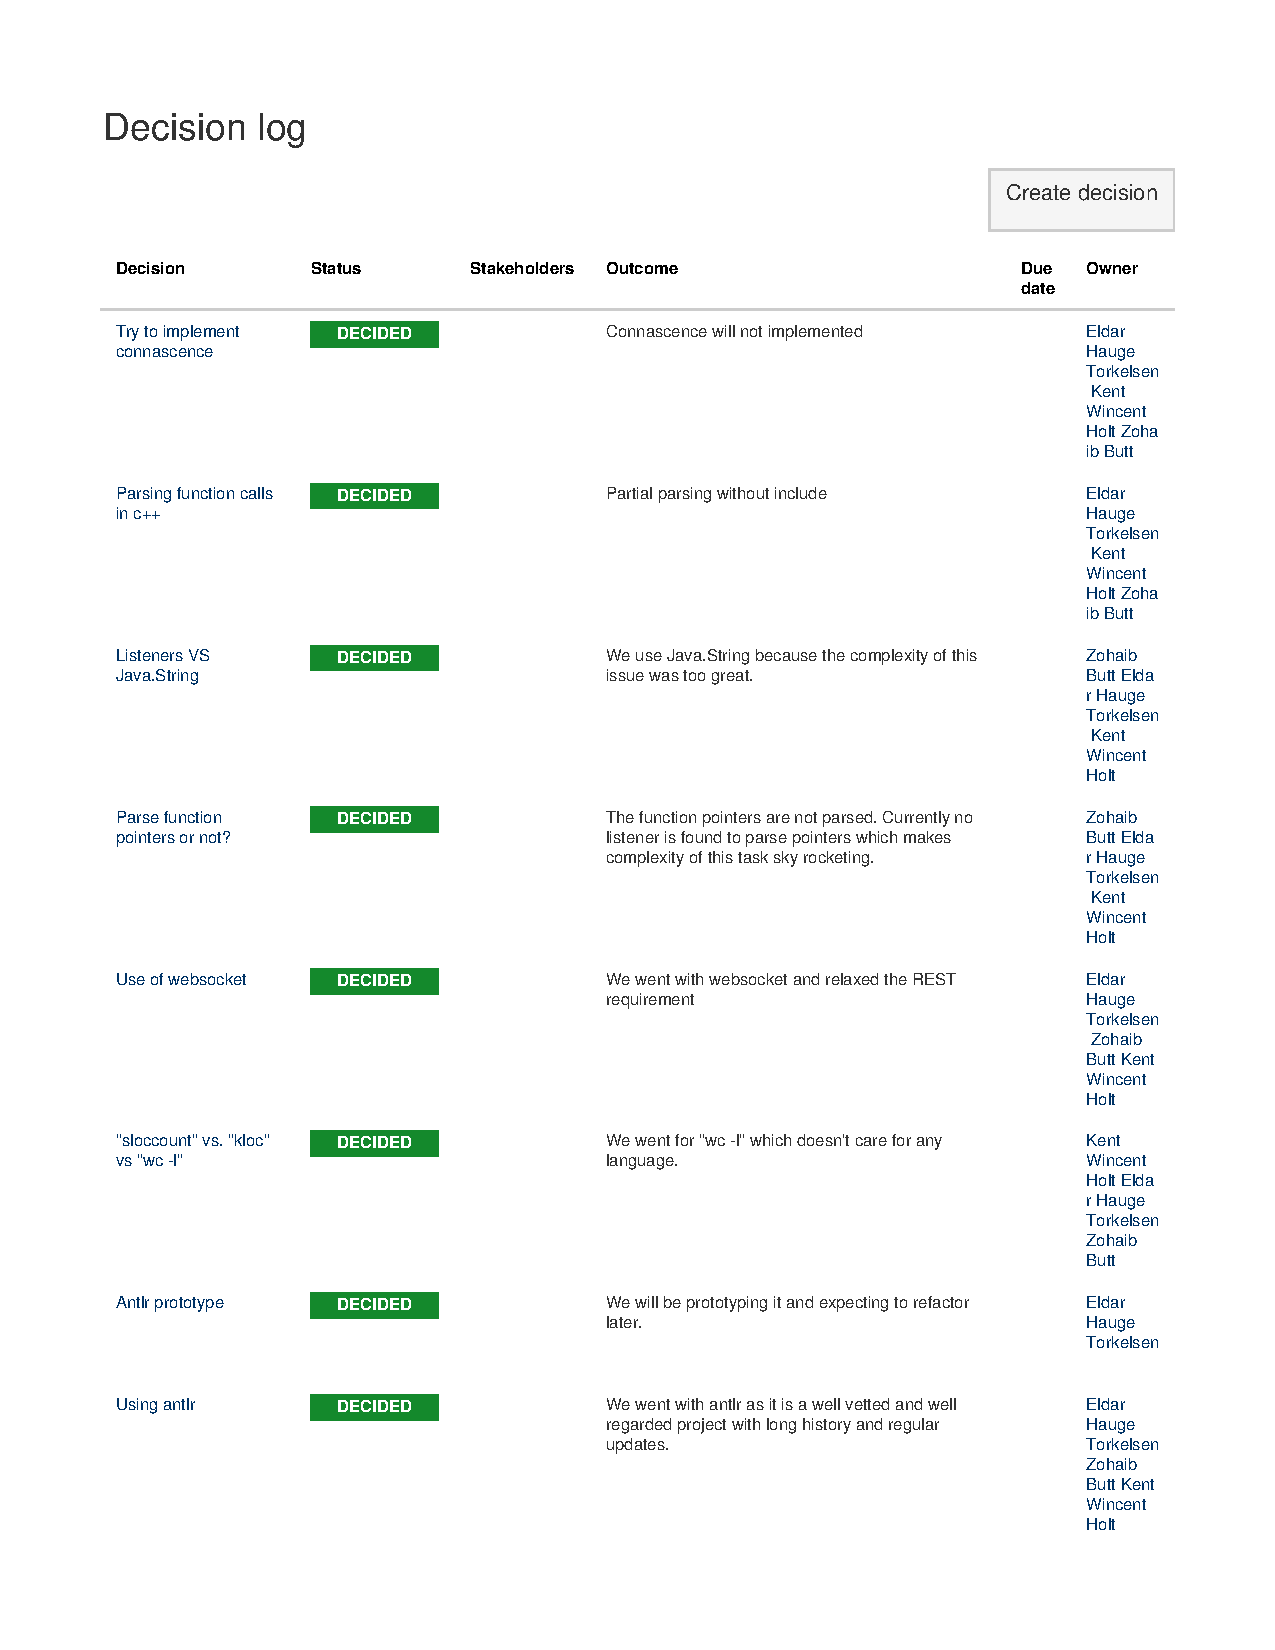
\includepdf[pages={-}]{inc/generalAppendix/jiraDecisionlog.pdf}
\chapter{Meeting Logs}
\section*{Meeting with Supervisor}

\subsection*{Participants}

\textbf{Convener}: \supervisor{} \\
\textbf{Facilitator}: \facilitator{}  \\
\textbf{Recorder}: \scrummaster{}  \\
\textbf{Others}                            \\
\textbf{Absent}: \groupleader{}

\subsection*{Agenda}
\begin{itemize}
    \item Feedback on report draft
    \item What should be the title of the development model and related topics?
    \item What should we do regarding the open task description? 
    \item What is the difference between subject area and background section?
    \item What should we do with the effect and result goals?
    \item Can we change the project plan during the development?
    \item What should be added to the apendix?
    \item What development method should we use with DevOps?
    \item do we lack any group roles?
\end{itemize}

\subsection*{Minutes}

\subsubsection*{Feedback on report draft}

Not much to say, it is overall ok. Regarding the rutines you should add what will happen if rules are broken.
An example could be 3 days without working gives a warning before talking with me (supervisor). 

\subsubsection*{What should be the title of the development model and related topics?}
You don't need to use the original title, make a new one for yourself.

\subsubsection*{What should we do regarding the open task description? }
Discuss with the product owner, try to extract more information. Talk about what you expect should be the requirements and go from there.

\subsubsection*{What is the difference between subject area and background section?}
There is not much of a difference, what you got now seem to be ok.

\subsubsection*{What should we do with the effect and result goals?}
result goals is what you deliver on the last day whilst effect goals is the effect of the program in action after delivery. You won't have the chance to verify that it's effect are good enough. Don't set error message as a result goals as those are expected anyway.

\subsubsection*{Can we change the project plan during the development?}
Yes, try to make it as specific as possible now, but as you are using an agile development method, you should change it later. Might want to have a old and new version of the plan to compare at the end.

\subsection*{What should be added to the apendix?}
You should add meeting summary and time log but not things like commit log or change log.

\subsubsection*{What development method should we use with DevOps?}
That is up to you. Scrum, as you have mentioned, is a good idea but you should look at other alternatives to.

\subsubsection*{do we lack any group roles?}
You only lack those that are specific for the development method you chose. 

\newpage
\section*{Internal meeting}

\section*{Participants}

\textbf{Convener}: \groupleader{}     \\
\textbf{Facilitator}: \facilitator{}  \\ 
\textbf{Recorder}: \scrummaster{}   \\ 
\textbf{Others}                    \\

\section*{Agenda}
\begin{itemize}
    \item Preparation for Christopher meeting
    \item Preparation for Kolloen meeting
\end{itemize}

\section*{Minutes}

\subsection*{Preparation for Christopher meeting}

We need more concrete specifications for the task in order to write a good report. The problems mostly regard requirements and risks. We should make a drawing of how we see the system and confirm with him that our vision does not contradict his. Might want to mention how the nodes in the 3d view has gravity towards each other and towards meddle based on number of connections and connections to each other.

\subsection*{Preparation for Kolloen meeting}

I will be a short meeting as we talked with him on thursday.
We need to ask about the gant diagram as we are using scrum. The risk analysis should also be discussed.  

We still have to do task devision, plan for handling important risk and development plan. We should probably have done a bit of that before the meeting.

\subsection*{Other}

We should probably work more efficiently, we spend too much time talking.

\newpage
\section*{Meeting with Supervisor}

\subsection*{Participants}

\textbf{Convener}: \supervisor{}\\
\textbf{Facilitator}: \facilitator{}  \\
\textbf{Recorder}: \scrummaster{}  \\
\textbf{Others}: \groupleader{} \\
\textbf{Absent}:

\section*{Agenda}
\begin{itemize}
    \item Feedback on report draft
\end{itemize}

\section*{Minutes}

\subsubsection*{Feedback on report draft}
Ikke lenge siden sist så det er ikke noe å si.
I forhold til raporten, si ifra hvilke seksjoner jeg skal se på.

\subsubsection{Om gant}
Det er greit å bruke burndown chart istedet for gant.

\subsubsection{Risk managment}
Vi har nevnt 10 risk managment og lurte på om du kunne i noe tilbakemelding.
Bør nok legge til hva som kommer til å skje hvis noen blir syke. 

\subsubsection*{Hva en ofte bommer på}
Ofte bruker folk for lang tid på å lære noe nytt. begynn med det en ikke kan fra før. En har bedre tid til å lære det.

\subsubsection*{Framework}
view.js som frontend rammeverk. Angular er vanskeliggere å sette se inn i. Polymer bør sjekkes ut også. 

\subsubsection*{Hva bør gjøres mer på}
Fyll ut helt på alt. Før ta dette mer på mandag når siste gjennomgang skal være.

\subsubsection*{Design i planleggings fasen}
Ikke ta med design nå. (ikke legg til bilder nå)

\subsubsection*{Other}
Skal userstudy legges til som vedlegg. Viktigste punkter fra studies kan tas med i rapporten.

\newpage
\section*{Meeting with Product owner}

\subsection*{Participants}
\textbf{Convener}: \productowner{}\\
\textbf{Facilitator}: \facilitator{}  \\
\textbf{Recorder}: \scrummaster{}  \\
\textbf{Others}: \groupleader{} \\
\textbf{Absent}: 

\subsection*{Agenda}
\begin{itemize}
    \item Specific constraints to include.
    \item Open stack for deployment.
    \item MIT License.
    \item Interactions.
    \item Expected systems effect. 
    \item Worries.
    \item other.
\end{itemize}

\subsection*{Minutes}

\subsubsection*{Specific constraints to include}

Should check out juristical constraints yourself.
should work with gitrepo but would also be nice for it to work on zip files.

\subsubsection*{Open stack for deployment}
Would not like OpenStack as a dependencies, docker would be nice. would be nice to be able to run it on "My machine". 

\subsubsection*{MIT License}

Perfect.

\subsubsection*{Interactions}

Open collapse like makes sense in 2D is most important other ideas are also good. Must always be able backtrack.

For the gathering of related datastructures we should check out force directed algorithms.
\subsubsection*{Expected systems effect}

Should be able to be used in a classroom setting where all students use the system at a time.

\subsubsection*{Worries}

You should not focus on worry, just try to learn as much as possible.

\subsubsection*{Other}

For the quality metrics we should check out cyclomatic complexity and connascence metrics. \\
We should also check out profiling and software quality tools as used by other IDEs like visual studio. 
\\
\\
Kotlin would be nice for mobile programming. \\
Would be nice to have an exposed POSIX API for accessing data without visualizations and be able to choose what information these requests should contain, in the sense of static analysis data, quality metrics data and/or connectivity data.

\newpage
\section*{Meeting with Supervisor}

\subsection*{Participants}

\textbf{Convener}: \supervisor{}\\
\textbf{Facilitator}: \facilitator{}  \\
\textbf{Recorder}: \scrummaster{}  \\
\textbf{Others}: \groupleader{}                         \\
\textbf{Absent}: 

\subsection*{Agenda}
\begin{itemize}
    \item Feedback on report draft

\end{itemize}

\subsection*{Minutes}

\subsubsection*{Feedback on the report}
The introduction should be more general, making it more specific later on. Changing it from "Finding libraries or frameworks" to "analyzing source code". 
There is too much use of the word "Should". The report is meant to be binding and contain what must be done. If additional should be added, then that should be clearly separated.

% fixed
There is a grammatical error in 2.3.1. 


In 3.1, when talking about the development process, it gets a bit too loose. You should add where in this section your project acts. Don't just add this in "bounds".

When you mention that the system can be useful for documenting, this conflicts with the usecase being for identifying good libraries and framework.

It's a bit confusing when you use the words "Data structure" and "function" interchangeably. 

In terms of risk analysis, you have set that one or more members of group are unavailable for a long period of time as priority 7, but have not set up a mitigation for this. 
Add priority column on "mitigation table". 

Version Lava lizard and version 1.0, before "all development should be done in the middle of April"; It's ok to have time to write on the report. But the quantity you have added is more than usual. Usually one only allocates 2-4 weeks.

Your user studies have been set up with a lot of other stuff. It would be better if it was mentioned how much time is used on that part, as now it looks like there is not enough time.

This is a complex thesis, It is important to do user study in correct manners. User studies is a hard process and we as developers do not have much experience in this topic. Usually the user studies requires 5 - 20 users and more than a week to be properly planned and conduct.

It seems strange that we will be doing all analysis ourselves. Could look into "Sonar qube" for a part of analysis.

It would be better if its added that you will find software to do part of the features for us.

Supervisor will find out the delivery data of bachelor thesis.

Supervisor does not know any automatic usability and accessibility tool.

\newpage
\section*{Meeting with Product owner}

\subsection*{Participants}
\textbf{Convener}: \productowner{}\\
\textbf{Facilitator}: \facilitator{}  \\
\textbf{Recorder}: \scrummaster{}  \\
\textbf{Others}: \groupleader{} \\
\textbf{Absent}: 

\subsection*{Agenda}
\begin{itemize}
    \item Feedback
\end{itemize}

\subsection*{Minutes}
Its ok to say "you don't have webgl, good luck".
I would suggest you try to find out what the tricky parts are and chose your libraries around that.

I think it should be made future proof, so don't use angular. Could look into react native but the focus should be on the webgl part. Do the webgl part well and the rest is not important. You need systematic decisioning to show why you went for a framework/libraries.

For the first sprint use it for trying out different things and figuring out what works.

\newpage
\section*{Meeting with Supervisor}

\subsection*{Participants}

\textbf{Convener}: \supervisor{}\\
\textbf{Facilitator}: \facilitator{}  \\
\textbf{Recorder}: \scrummaster{}  \\
\textbf{Others}: \groupleader{}                          \\
\textbf{Absent}: 

\subsection*{Agenda}
\begin{itemize}
    \item Feedback on report draft

\end{itemize}

\subsection*{Minutes}
Raporten ble godkjent og virker bra.
Viktigste er at dette  er et verktøy for dere.

Fristen for innlevering er nå riktig i studentweb, dere vet når dere skal levere.


Det som er vikti er at dere noterer alle avgjørelser underveis. Det er viktig for slutt raporten. Ja, det kan være nok med sprint review meetings for dette, i og med at dere har ukentlige sprint. Dette er den største feilen folk gjør. 


De delene av prosjektet synes er vanskelig, begynn med det. Det som er trivielt kan dere ta senere. 

Vi tenker å bruke Threejs er dette bra?
svar: Vet ikke, gjør ikke så mye med den delen av utvikling. Bare husk å skrive hvorfer dere tok dette valget. hvis det viser seg å ha svakheter er det da enklere å forklare til slutt.

Bruk produktet dere lager til å sjekke alternativer for Three.js for demonstrasjon.

\newpage
\section*{Meeting with Supervisor}

\subsection*{Participants}

\textbf{Convener}: \supervisor{}\\
\textbf{Facilitator}: \facilitator{}  \\
\textbf{Recorder}: \scrummaster{}  \\
\textbf{Others}:                           \\
\textbf{Absent}: \groupleader{}

\subsection*{Agenda}
\begin{itemize}
    \item Feedback on report draft

\end{itemize}

\subsection*{Minutes}
Dere ligger bak, men det er ikke unormalt etter første sprint. Det er ikke så stort problem hvis dere kan hente dere inn og når dere bruker 1 ukes sprint. 

Det at devops delen ikke er oppe er ikke noe stort problem, det kommer. 

\newpage
\section*{Meeting with Product owner}

\subsection*{Participants}
\textbf{Convener}: \productowner{}\\
\textbf{Facilitator}: \facilitator{}  \\
\textbf{Recorder}: \scrummaster{}  \\
\textbf{Others}: \groupleader{} \\
\textbf{Absent}: 

\subsection*{Agenda}
\begin{itemize}
    \item Feedback
\end{itemize}

\subsection*{Minutes}
As an opening, we estimate that we are 1 day behind.
response: Thats not a worry, there will be more like that. 

We had some problems with imgui, The functionality is there but the boxes are black. 
We should talk to Per Morten as he has experience with imgui, but not with js binding.

We had problems with antlr, it was made in java but has golang target but that is in development. We went with java version. 

We have set up the server, no testing yet and it took longer than expected. 

We will have problems that others don't as your project is entierly different from the other projects. Don't worry too much. 

next sprint will be "representation of complex datastructures". Seems good, don't get too discuraged if you can't make too complex structures. Would be nice with multilevel structures and trees. 


Not a fan of npm. Breaks often. Its a possibility but would prefer a lightweight option for important dependencies. 

\newpage
\section*{Meeting with Supervisor}

\subsection*{Participants}

\textbf{Convener}: \supervisor{}\\
\textbf{Facilitator}: \facilitator{}  \\
\textbf{Recorder}: \scrummaster{}  \\
\textbf{Others}                            \\
\textbf{Absent}: \groupleader{}

\subsection*{Agenda}
\begin{itemize}
    \item Feedback on report draft

\end{itemize}

\subsection*{Minutes}

\subsubsection*{Feedback on report draft}
Ligger fremdeles back, har hentet in en god del av det vi tapte på første sprint. Ikke brenn all kruttet nå. 70 timers uker greier dere ikke hele veien. 

Under sprinten fikk vi problemer med csp/ origin policy. 

Hvis vi styrer både server og client, kan vi sette i headeren en ip range. Så det skal være overkommelig.
Vi har brukt.

Vi bruker nå en frontend server og en rest api. 
Vi må fike opp i bruken av http og https. 

Vi har ikke fått skrevet noe på raporten men det skal gå bra hvis vi bare skiver ned viktige avgjørelser.
Status raportene sendes bare til 

\newpage
\section*{Meeting with Product owner}

\subsection*{Participants}
\textbf{Convener}: \productowner{}\\
\textbf{Facilitator}: \facilitator{}  \\
\textbf{Recorder}: \scrummaster{}  \\
\textbf{Others}: \groupleader{} \\
\textbf{Absent}: 

\subsection*{Agenda}
\begin{itemize}
    \item Feedback
\end{itemize}

\subsection*{Minutes}
Update from last sprint, we were 3 days behind. now we are 1 day behind after 212 hours. We can now display somthing, but currently broken by backend changes. 

Currently the 3D force directed graph works, but we dont use backend data yet (soon).  The algorithm is not a library, we implemented it but we might change and make it a dependency due to some limitations. 

The force is calculated as individual links between each node, other implementations use a global force instead. 

There could be complications with this as larger systems might collapse. Will probably need to be revisited often throughout the project. Interesting. "Can of worms". Should bear in mind that attraction change over distance. We have done this. 

The json model sendt from the backed duplicates with multiple scopes. While looking into it check how to see what you can get from parts, try to do it so you dont need to revisit the schema. We are looking into listeners and visitors. 

The parsing takes a long time, should do some chaching, and delete things that are not used for a long time.

Including imgu creates a dependency on emscripten and use of npm for now.

We should probably spend time in the upcomming sprint on working on the frontend, refactoring it as now if multiple were to work on it, there is bound to be major conflicts. The Antler scope problem is kind of a major blocker, but with data mocking we should be able to get past that.

\newpage
\section*{Retrospective meeting}
\subsection*{Participants}

\textbf{Convener}:\scrummaster{} \\
\textbf{Facilitator}: \facilitator{}  \\
\textbf{Recorder}: \scrummaster{} \\
\textbf{Others}: \groupleader{} \\
\textbf{Absent}: 

\subsection*{Agenda}
\begin{itemize}
    \item What went well?
    \item What could have been done better?
    \item Is there something new that the team wants to start doing?
    \item Is there something that puzzles us?
\end{itemize}

\subsection*{Retrospective}

\noindent

\par

\begin{Parallel}[v]{0.48\textwidth}{0.48\textwidth}
\ParallelLText{\noindent

\textbf{What did we do well?}
\begin{itemize}[rightmargin=.52\textwidth]
\item{The group worked well and was able to make of for much of the time lost in the last sprint.}
\item{The group was able to integrate GUI framework ahead of schedule.}
\item{Backend was refactored to a stage where it could be used for the sprint.}
\item{The team learnt about antlr quicker than anticipated.}
\end{itemize}
}
\ParallelRText{\noindent

\textbf{What should we have done better?} 
\begin{itemize}[rightmargin=.52\textwidth]
  \item{The group was forced to work overtime to the point of exhaustion.}
  \item{Could not immediately find a good force directed graph library/algorithm that would take the input data we required.}
  \item{There was very little time to document code or creating tests.}
  \item{The group realized late that their parser implementation was not sufficient.}
  \item{The estimations of time reacquired per task was significantly off.}
  \item{The tasks conflicted forcing members to do pair programming on relatively simple programming components.}
\end{itemize}

}
\ParallelPar
\end{Parallel}

\subsection*{Is there something new that the team wants to start doing?}
The team will divide the stories further so that each member can be expected to finish several by the end of the sprint and prevent working in the same part of the code base. The tasks should also be clarified better and be more concise.

\subsection*{ Is there something that puzzles us?}
We need to look into Antlr visitor versus Antlr listeners. 
We should look into professional frontend and file structure as well as programming patterns.
We might have problems with latency and computational complexity.
\newpage

\section*{Meeting with Supervisor}

\subsection*{Participants}

\textbf{Convener}: \supervisor{}\\
\textbf{Facilitator}: \facilitator{}  \\
\textbf{Recorder}: \scrummaster{}  \\
\textbf{Others}:\groupleader{}    \\
\textbf{Absent}: 

\subsection*{Agenda}
\begin{itemize}
    \item Feedback on report draft

\end{itemize}

\subsection*{Minutes}

\subsubsection*{Feedback on report draft}
Nåværende status er at vi fremdeles er 1 dag etter. Dette er ikke noen krise, men tenk på hvor mye dere legger i sprinten. Er nok mer interessant med arbeidsvekten. 

Ligger nok litt bak på raportskriving

\newpage
\section*{Meeting with Product owner}

\subsection*{Participants}
\textbf{Convener}: \productowner{} \\
\textbf{Facilitator}: \facilitator{}  \\
\textbf{Recorder}: \scrummaster{}  \\
\textbf{Others}: \groupleader{} \\
\textbf{Absent}: 

\subsection*{Agenda}
\begin{itemize}
    \item Feedback
\end{itemize}

\subsection*{Minutes}
We have less to talk about this time as its mostly re factoring. We did not change much in the general structure, we looked up how to structure with a module pattern and android studio  like approach with string localization and style. We found a solution for figuring out where in the scope we are using a simple stack and a tree structure. We should document our decisions.

We currently have scopes working for only namespaces and there is duplication on cpp files. 

Could have a force directed graph on the captions of the nodes (The name labels). 

The size of the objects could be based on the number of lines and complexity. 

We should check for informal user-studies or ethic's board for formal user-studies. We need concrete feedback. It seem to be more on the side of informal studies. 

We don't need compliance form if we don't collect user-data or want to cite a person directly. 

For the next sprint we had planned meta-data and multidimensional variables, we won't be able to finish this but we will go in this direction. We should focus on the meta-data and cohesion, make it easier for users to understand what is happening.

\newpage
\section*{Retrospective meeting}
\subsection*{Participants}

\textbf{Convener}:\scrummaster{} \\
\textbf{Facilitator}: \facilitator{}  \\
\textbf{Recorder}: \scrummaster{} \\
\textbf{Others}: \groupleader{} \\
\textbf{Absent}: 

\subsection*{Agenda}
\begin{itemize}
    \item What went well?
    \item What could have been done better?
    \item Is there something new that the team wants to start doing?
    \item Is there something that puzzles us?
\end{itemize}

\subsection*{Retrospective}

\noindent

\par

\begin{Parallel}[v]{0.48\textwidth}{0.48\textwidth}
\ParallelLText{\noindent

\textbf{What did we do well?}
\begin{itemize}[rightmargin=.52\textwidth]
    \item{The stories were divided into multiple small tasks, which made development very efficient.}
    \item{The group improved with holding 8 hours limit for work day.}
    \item{Code quality became better, as we learned JavaScript and did not care about backwards compatibility beyond WebAssembly.}
    
\end{itemize}
}
\ParallelRText{\noindent

\textbf{What should we have done better?} 
\begin{itemize}[rightmargin=.52\textwidth]
    \item{We should have worked more efficiently with the front-end refactoring.}
    \item{The slow refactoring made it hard to complete other tasks.}
    \item{The refactoring covered a lot of files and made for a difficult merge.}
\end{itemize}

}
\ParallelPar
\end{Parallel}

\subsection*{Is there something new that the team wants to start doing?}
We will focus heavier on setting up sub-tasks as smaller tasks proved use-full in previous sprint.

\subsection*{ Is there something that puzzles us?}
We should look more into user-studies, as we had not considered the ethics board required for formal user-studies.

\newpage
 
\section*{Meeting with Supervisor}

\subsection*{Participants}

\textbf{Convener}: \supervisor{}        \\
\textbf{Facilitator}: \facilitator{}    \\
\textbf{Recorder}: \scrummaster{}       \\
\textbf{Others}                         \\
\textbf{Absent}: \groupleader{}

\subsection*{Agenda}
\begin{itemize}
    \item Feedback on report draft
    \item What should be the title of the development model and related topics?
    \item What should we do regarding the open task description? 
    \item What is the difference between subject area and background section?
    \item What should we do with the effect and result goals?
    \item Can we change the project plan during the development?
    \item What should be added to the apendix?
    \item What development method should we use with DevOps?
    \item do we lack any group roles?
\end{itemize}

\subsection*{Minutes}

Hva skal vi gjøre for status raporten?
Veldig uformelt dokument. Bare skriv om hvordan dere ligger an. skir om diskusjoner dere har hatt, problemer og aha oplevelser. 
Vi har fulgt rådet med websocket, det virker som det går greit annet enn at coden virker mye mer uoversiktlig, vi vet ikke hellt hvordan vi kan fikse det. Det er et krav om at vi bruker REST, skal snakke med arbeidsgiver for å sjekke om dette er greit. Vi forbedrer oss med scrum via å dele opp oppgaver bedre, men estimering er fremdeles ikke bra.
\newpage
\section*{Meeting with Product owner}

\subsection*{Participants}
\textbf{Convener}: \productowner{}      \\
\textbf{Facilitator}: \facilitator{}    \\
\textbf{Recorder}: \scrummaster{}       \\
\textbf{Others}: \groupleader{}         \\
\textbf{Absent}: 

\subsection*{Agenda}
\begin{itemize}
    \item Feedback
\end{itemize}

\subsection*{Minutes}
We have used a websocket witch is in conflict with the requirement for REST api.
REST api criteria has been loosened, the idea is to have it available at all times.

We found that figuring out what functions call what won't be trivial. It can contain nested structures recursively. We will be able to solve it, but it might take a long time to add this feature. We work on seperate tasks, but have a low threshold for getting help from other groupmembers. 

We should look into interpreter pattern. 

If we use external parties for quality metrics, then we need to make sure we can submit code snippets(function level) and not whole projects. 
\newpage
\section*{Retrospective meeting}
\subsection*{Participants}

\textbf{Convener}:\scrummaster{} \\
\textbf{Facilitator}: \facilitator{}  \\
\textbf{Recorder}: \scrummaster{} \\
\textbf{Others}: \groupleader{} \\
\textbf{Absent}:

\subsection*{Agenda}
\begin{itemize}
    \item What went well?
    \item What could have been done better?
    \item Is there something new that the team wants to start doing?
    \item Is there something that puzzles us?
\end{itemize}

\subsection*{Retrospective}

\noindent

\par

\begin{Parallel}[v]{0.48\textwidth}{0.48\textwidth}
\ParallelLText{\noindent

\textbf{What did we do well?}
\begin{itemize}[rightmargin=.52\textwidth]
    \item{The team worked in average 8 hours a day.}
    \item{Team was able to finish most of the issues for the sprint.}
    \item{Team is getting better in dividing big stories into sub small stories.}

\end{itemize}
}
\ParallelRText{\noindent

\textbf{What should we have done better?} 
\begin{itemize}[rightmargin=.52\textwidth]
    \item{We should have estimated sub stories to manage time better.}
    \item{We should have completed informal user studies.}
\end{itemize}

}
\ParallelPar
\end{Parallel}

\subsection*{Is there something new that the team wants to start doing?}
We will start estimating sub-tasks as well as stories and epics.

\subsection*{Is there something that puzzles us?}
We might have problems relating function declaration to function call and definition when they are in different parts of the program. 

\newpage

\section*{1st Statusreport}

\section*{Participants}

\textbf{Convener}: \groupleader{}     \\
\textbf{Facilitator}: \facilitator{}  \\ 
\textbf{Recorder}: \scrummaster{}   \\ 
\textbf{Others}                    \\

\section*{Summary}
As of the \nth{8} of March, we are behind schedule due to the complexity of parsing and quantity of new technologies the team had to learn. 

We haven't been able to write tests for any functionality, due to functionality taking precedence over tests and the misestimation of stories. Stories have in most cases been underestimated and not divided or concrete enough. 

Despite this, the progression is still good and we expect to have a good product by the end of the development phase. 

So far we parse and handle namespaces, functions, packages/using namespaces and partially classes for both Java version 9 and C++ version 14.

\section*{Challenges}
Parsing programming languages turned out to be more complicated than expected. We were using Antlr, but could not use its generated go code due to embedded Java being required in the grammar file to describe the programming language. As an example of Antlr complexity, if you want to find the function identifier/name through a class declaration, then you might have to go through a structure with 10 distinct contexts where 4 are called recursively. Simplifying this was done through handling scopes separately. It was difficult to make the parser in such a way that we could separate scopes and refactored several times ending with us using a stack based implementation. Where stack will give us what scope model we are parsing so we can add the data found in the scope model.

We also underestimated the effort required to do user-studies, so this has been postponed for now. Every time we intended to follow through with our user-studies schedule, we found that slight changes would make the studies significantly informational and help-full. One such slight change was to add links for calls in the 3D representation, but this proved significantly more difficult than expected as to identify overloaded functions and class member functions, we were required to also parse name-spaces and variables with their types.

The adding and parsing took a lot of time for multi-file repositories. The user would see the loading circle without any feedback on status of the system. To fix this we decided to send the API request using websocket protocol so that client and server could communicate while server is parsing.

\section*{Accomplishment}
We have a working minimum viable product that partially parses functions, namespaces, classes and variables of the submitted repository and displays basic information about the project. 

The API is currently partially implemented. It has 4 possible endpoints which is Adding of repository, initial request, Listing of stored repositories and fetching implementation of a function.

For visualization of different data structures we decided to use forced directed graph to show the strong/weak relations between nodes. We are also thinking to apply level of detail, where one can zoom in to a node on the graph and a seperate 3D space will be initialized showing a graph containing data structures within the node scope. This will require rework on current implementation of forced directed graph.

\section*{Upcoming}
We are currently looking into more complicated quality metrics, like Connascence metrics, Halstead complexity measures, Cyclic complexity and programs like Sonarqube that might help us calculate these metrics easier.
Later we will change the 3D representation to better reflect scopes in the parsed code and window management to make it easier for end-user to navigate and control the application. 
\newpage
\section*{Meeting with Product owner}

\subsection*{Participants}
\textbf{Convener}: \productowner{}\\
\textbf{Facilitator}: \facilitator{}  \\
\textbf{Recorder}: \scrummaster{}  \\
\textbf{Others}: \groupleader{} \\
\textbf{Absent}: 

\subsection*{Agenda}
\begin{itemize}
    \item Feedback
\end{itemize}

\subsection*{Minutes}
We have added a front page with description and supported browsers and current features handled. 
We have websocket finished and giving more info about status user.

Would be nice to make it possible to compare different repositories. Would be nice to be able to change between different repos and retain state. 
We need to consider memory at this point.

We will continue with function calls and class parsing. In addition we would like to represent the scopes on front end. In addition we have looked at connacence and cliometric, metrics. Found a related one for Halstead complexity measures. 

If we do user studies, we need to try to get around gdpr and have it offline. It would be difficult to go for the entirely formal approach requiring questions to be submitted and confirmed through a process taking over a month. 

We are worried about the complexity of figuring out functions as in c++ its tightly connected to the data. 


\newpage
\section*{Retrospective meeting}
\subsection*{Participants}

\textbf{Convener}:\scrummaster{} \\
\textbf{Facilitator}: \facilitator{}  \\
\textbf{Recorder}: \scrummaster{} \\
\textbf{Others}: \groupleader{} \\
\textbf{Absent}:

\subsection*{Agenda}
\begin{itemize}
    \item What went well?
    \item What could have been done better?
    \item Is there something new that the team wants to start doing?
    \item Is there something that puzzles us?
\end{itemize}

\subsection*{Retrospective}

\noindent

\par

\begin{Parallel}[v]{0.48\textwidth}{0.48\textwidth}
\ParallelLText{\noindent

\textbf{What did we do well?}
\begin{itemize}[rightmargin=.52\textwidth]
    \item{Stories were described better.}
\end{itemize}
    
}
\ParallelRText{\noindent

\textbf{What should we have done better?} 
\begin{itemize}[rightmargin=.52\textwidth]
    \item{Should have focused more on the stories at hand}
    \item{Estimates were far off and the complexity turned out to be significantly higher than expected}
    \item{Several stories were set as sub-tasks that should have been stories}
\end{itemize}
    
}
\ParallelPar
\end{Parallel}

\subsection*{Is there something new that the team wants to start doing?}
Better division between epics, stories and sub-tasks. 


\subsection*{Is there something that puzzles us?}
Complexity and flexibility of languages is scary and puzzles us a lot.
Amount nested if/else if statements increase day by day and this might cause a problem for unit testing.

\newpage

\section*{Meeting with Product owner}

\subsection*{Participants}
\textbf{Convener}: \productowner{}\\
\textbf{Facilitator}: \facilitator{}  \\
\textbf{Recorder}: \scrummaster{}  \\
\textbf{Others}: \groupleader{} \\
\textbf{Absent}: 

\subsection*{Agenda}
\begin{itemize}
    \item Feedback
\end{itemize}

\subsection*{Minutes}
We are still struggling with parsing functions, we have refactored from multiple conditionals to instead use listeners. We also try to debug by using reflection to find out what we have available and what it will return. 

At this point we can think about standardizing a middle layer to make it easier to add new languages later.

We are thinking to only parse one language from now as we have found that our approach would work for multiple languages without problem. If we continue with only one language from now we could focus on other aspects. 

The java grammar is very good and made by the one who made antlr and follow the specifications. 

We will still make as much as possible language independent. 
\newpage
\section*{Retrospective meeting}
\subsection*{Participants}

\textbf{Convener}:\scrummaster{} \\
\textbf{Facilitator}: \facilitator{}  \\
\textbf{Recorder}: \scrummaster{} \\
\textbf{Others}: \groupleader{} \\
\textbf{Absent}:

\subsection*{Agenda}
\begin{itemize}
    \item What went well?
    \item What could have been done better?
    \item Is there something new that the team wants to start doing?
    \item Is there something that puzzles us?
\end{itemize}

\subsection*{Retrospective}

\noindent

\par

\begin{Parallel}[v]{0.48\textwidth}{0.48\textwidth}
\ParallelLText{\noindent

\textbf{What did we do well?}
\begin{itemize}[rightmargin=.52\textwidth]
    \item{We managed to refactor the back-end to use listeners instead of huge nested if statements code blocks.}
    \item{We managed to change the structure on front-end to use trees instead of arrays for force directed graph and parsing.}
\end{itemize}
    
}
\ParallelRText{\noindent

\textbf{What should we have done better?} 
\begin{itemize}[rightmargin=.52\textwidth]
    \item{At no point should the group be expected to work for 200 hours in one week.}
    \item{Estimation was far off, the stories that were expected to be almost done from previous sprint are still a problem.}
\end{itemize}
    
}
\ParallelPar
\end{Parallel}
\subsection*{Is there something new that the team wants to start doing?}
The team wants to have a sprint that focuses heavily on testing as that has not been prioritized. 

\subsection*{Is there something that puzzles us?}
\label{appendix:retrospective2019-03-18}
Parsing function has puzzled us for the past 3 weeks, as C++ target functions are very flexible and can have anything in the body. We need a way to differentiate the function calls from the pointers assignment. Also keyword such as "this" is considered a function call no matter if the keyword is used to set a member variable or call a member function.
Function calls are difficult because they can be overloaded (so the parameter types are important), scoped (so what is in front of the identifier is important), and can be called with objects whose scope is declared elsewhere. 
\newpage

\section*{Meeting with Product owner And supervisor}
\subsection*{Participants}
\textbf{Convener}: \productowner{}\\
\textbf{Facilitator}: \facilitator{}  \\
\textbf{Recorder}: \scrummaster{}  \\
\textbf{Others}: \groupleader{} \\
\textbf{Absent}: 

\subsection*{Agenda}
\begin{itemize}
    \item Feedback
\end{itemize}

\subsection*{Minutes}
Life is good, yet bachelor is going slowly. We have used the week for testing. It goes slower than expected partially because we are using multiple systems with multiple testing environments, (AVA .js, go test .go and j-unit .java). We have some problems with j-unit as its difficult to mock with antlr. We have found a few bugs as a result of testing, like URI validation and unnecessary Fatal instead of error call. 
We have productively 2 weeks of development left which can cause a problem for the amount of work left. 
We want to Finnish scoping on front end, function calls, class parsing and cyclomatic complexity. Would be nice with cashing as well and  possibility of only saving last "x" repose.

We should structure the report to show the testing as a quality assurance and note that everything before the point of test-writing is likely to work.

Both supervisor should probably be on the list, but it should be noted when Christopher became supervisor.

About unfinished quality metrics (connacense), we could mention the possible with definition in the background and mention them later and in the future work having a red thread through it. 
\newpage
\section*{Retrospective meeting}
\subsection*{Participants}

\textbf{Convener}:\scrummaster{} \\
\textbf{Facilitator}: \facilitator{}  \\
\textbf{Recorder}: \scrummaster{} \\
\textbf{Others}: \groupleader{} \\
\textbf{Absent}: 

\subsection*{Agenda}
\begin{itemize}
    \item What went well?
    \item What could have been done better?
    \item Is there something new that the team wants to start doing?
    \item Is there something that puzzles us?
\end{itemize}

\subsection*{Retrospective}

\noindent

\par

\begin{Parallel}[v]{0.48\textwidth}{0.48\textwidth}
\ParallelLText{\noindent

\textbf{What did we do well?}
\begin{itemize}[rightmargin=.52\textwidth]
    \item{The team managed to finish most of testing related issues.}
    \item{The tasks were divided well enough that unexpected hinders allow members to just change over to a different task until problems were resolved.}
    \item{The team realized that the complexity of previously written code was higher than expected.}
    
\end{itemize}
}
\ParallelRText{\noindent

\textbf{What should we have done better?} 
\begin{itemize}[rightmargin=.52\textwidth]
    \item{The team took longer than expected to setup testing environment}
    \item{Large portions of the previously written code did not lend itself to creating simple tests.}
\end{itemize}

}
\ParallelPar
\end{Parallel}

\subsection*{Is there something new that the team wants to start doing?}
The next sprint will focus on more complicated tasks so the team will hold pair programming sessions for increased productivity. Team has planned to spend about 8 hours per day on pair programming session til the issues are resolved and spend the rest of the time working on the testing related tasks individually if possible.

\subsection*{ Is there something that puzzles us?}
We are still worried about estimating the three most complicated tasks. We have tried to estimated them before and been significantly off. We hope the pair programming will help.

\newpage

\section*{Meeting with Product owner And supervisor}
\subsection*{Participants}
\textbf{Convener}: \productowner{}\\
\textbf{Facilitator}: \facilitator{}  \\
\textbf{Recorder}: \scrummaster{}  \\
\textbf{Others}: \groupleader{} \\
\textbf{Absent}: 

\subsection*{Agenda}
\begin{itemize}
    \item Feedback
\end{itemize}

\subsection*{Minutes}
For the last week we have been pair programming and gotten a lot of difficult tasks done. 
We should fix the problem where to many nameplates causing clutter. Could substitute clutters with number of nameplates or number of types. 

For setting up the thesis, we should structure it systematically like MDA (mechanics dynamics aesthetics), low level implementation or high level overview. We should also connect what we have done with the other subjects we have had.

We should think about delta-parsing but implement the "bigger fish to fry". 

We should talk about use of libraries vs standards. 

we should talk about complexity metrics and how this correlates with byte-code and not always source code/ face value.

For testing we can take names if they allow us to and quote them. 
We should allow for change in the rest api and give documentation by version.

We should talk about what we consider feature complete.
\newpage
\section*{Retrospective meeting}
\subsection*{Participants}

\textbf{Convener}:\scrummaster{} \\
\textbf{Facilitator}: \facilitator{}  \\
\textbf{Recorder}: \scrummaster{} \\
\textbf{Others}: \groupleader{} \\
\textbf{Absent}: 

\subsection*{Agenda}
\begin{itemize}
    \item What went well?
    \item What could have been done better?
    \item Is there something new that the team wants to start doing?
    \item Is there something that puzzles us?
\end{itemize}

\subsection*{Retrospective}

\noindent

\par

\begin{Parallel}[v]{0.48\textwidth}{0.48\textwidth}
\ParallelLText{\noindent

\textbf{What did we do well?}
\begin{itemize}[rightmargin=.52\textwidth]
    \item{The pair programming worked very well for parsing function calls task.}
    \item{The team managed to complete two complicated problems that had lasted for several sprints.}
    \item{The pair programming helped getting all members up to date with the different component.}
    
\end{itemize}
}
\ParallelRText{\noindent

\textbf{What should we have done better?} 
\begin{itemize}[rightmargin=.52\textwidth]
    \item{The pair programming went slowly when some group members were tired.}
    \item{The team should have followed the time stated in project plan a lot better.}
\end{itemize}

}
\ParallelPar
\end{Parallel}

\subsection*{Is there something new that the team wants to start doing?}
The team will be more open to pair programming and will let tired members work on their own tasks. 

\subsection*{ Is there something that puzzles us?}
We are still uncertain of how long the visualization of function calls will take. 

\newpage

\section*{Meeting with Product owner And supervisor}
\subsection*{Participants}
\textbf{Convener}: \productowner{}\\
\textbf{Facilitator}: \facilitator{}  \\
\textbf{Recorder}: \scrummaster{}  \\
\textbf{Others}: \groupleader{} \\
\textbf{Absent}: 

\subsection*{Agenda}
\begin{itemize}
    \item Feedback
\end{itemize}

\subsection*{Minutes}

We have gotten our Supervisor back.
We are starting on the thesis writing and won't do much with the development. 
We have gotten some pointers on structure for writing. 

For the state of the program, we are having problems with merging files, at least in c++ as it is a compiler level statement and not included in the antlr.
\newpage
\section*{Meeting with Supervisor}

\subsection*{Participants}

\textbf{Convener}: \supervisor{}        \\
\textbf{Facilitator}: \facilitator{}    \\
\textbf{Recorder}: \scrummaster{}       \\
\textbf{Others}  \groupleader{}         \\
\textbf{Absent}: 

\subsection*{Agenda}
\begin{itemize}
    \item Hvordan referere til programm beskrivelse?
    \item Hvordan referere til ntnu-template?
    \item Hvordan kan vi oppdatere overleaf cache? 
    \item Hvor skal vi skrive om bruken av module pattern?
    \item Hvordan minimere kodesnutter?
    \item Max lengde av kodesnutt?
    \item Oppset av neste møte?
\end{itemize}

\subsection*{Minutes}
\subsubsection{Hvordan referere til program beskrivelse?}
De er ikke arkivert på web, så det kan være vanskelig. Gjør så godt dere kan, bruk beskrivelse på nett. Author er emneansvarlig etterfuøgt av institutt. 

\subsubsection{Hvordan referere til ntnu-template?}
Normal gruppe referering mot github. Authors er man contributers, ikke ha med publisher.

\subsubsection{Hvordan kan vi oppdatere overleaf cache?}
Vet ikke, kan snakke med noen av lærerene som har mer med overleaf.

\subsubsection{Hvor skal vi skrive om bruken av module pattern?}
Module pattern er mest i implementasjon. Kan referere fra design delen ned til implementasjon.

\subsubsection{Hvordan minimere kodesnutter?}
Bruk ... med // comment, for å forkaler hva som blir gjort i delen.

\subsubsection{Max lengde av kodesnutt?}
Blir kansje litt mye når deg går over 20 linjer. Kan være det blir lengre noen ganger.

\subsubsection{Oppset av neste møte}
Onsdag kl 10.15. 

\newpage
\section*{Meeting with Supervisor}

\subsection*{Participants}

\textbf{Convener}: \supervisor{}        \\
\textbf{Facilitator}: \groupleader{}    \\
\textbf{Recorder}: \scrummaster{}       \\
\textbf{Others}                         \\
\textbf{Absent}: \facilitator{}

\subsection*{Agenda}
\begin{itemize}
    \item Feedback on report draft

\end{itemize}

\subsection*{Minutes}

Overordnet struktur ser veldig brra ut. Språket iforhold til å være akademisk er greit men det er noen sprøk blomster. Noe av det går på korrektur. 1.2 tredje avsnitt, var rett og slett vanskelig å lese. også siste avnitt under 1.2. siste setning i 1.3 er også litt tung å forstå hva som er meningen. Den er grei men unødvendig tung. Prøv å finne et annet ord for "unprofessional". 1.5 midt i avsnittet, setning med "more theorethical understanding of" prøv å omskrive. 

Når en nevner tidsbegrensing; ta med start tid, ikke bare slutt tid.
Opperasjonelle krav er veldig vanskelig å måle, må endres.  

risiko annalyse: må få riktig ordbruk for å vise hva som er sikkerhet i løsningen og hva som er sikkerhet i prosessen. Første krav nevner sikkerhetskrav, det er dette som er problemet. 

Ta sikkerhets aspectene ut av risk assessment.

31 arkitektur. første avsnitt nevner veldig mye, 

første avsnitt under backend er også veldig vanskelig å lese

under figur scrum board for test sprint, sier delt i fire når figuren viser 5 deler (Done).

Ser ikke ut til å være noen feil med forholdet mellom  implementation og development

deployment bør vøre etter implementatsjon når det er deploy på hardware.
\newpage


\chapter{Time log}
\label{app:timelog}
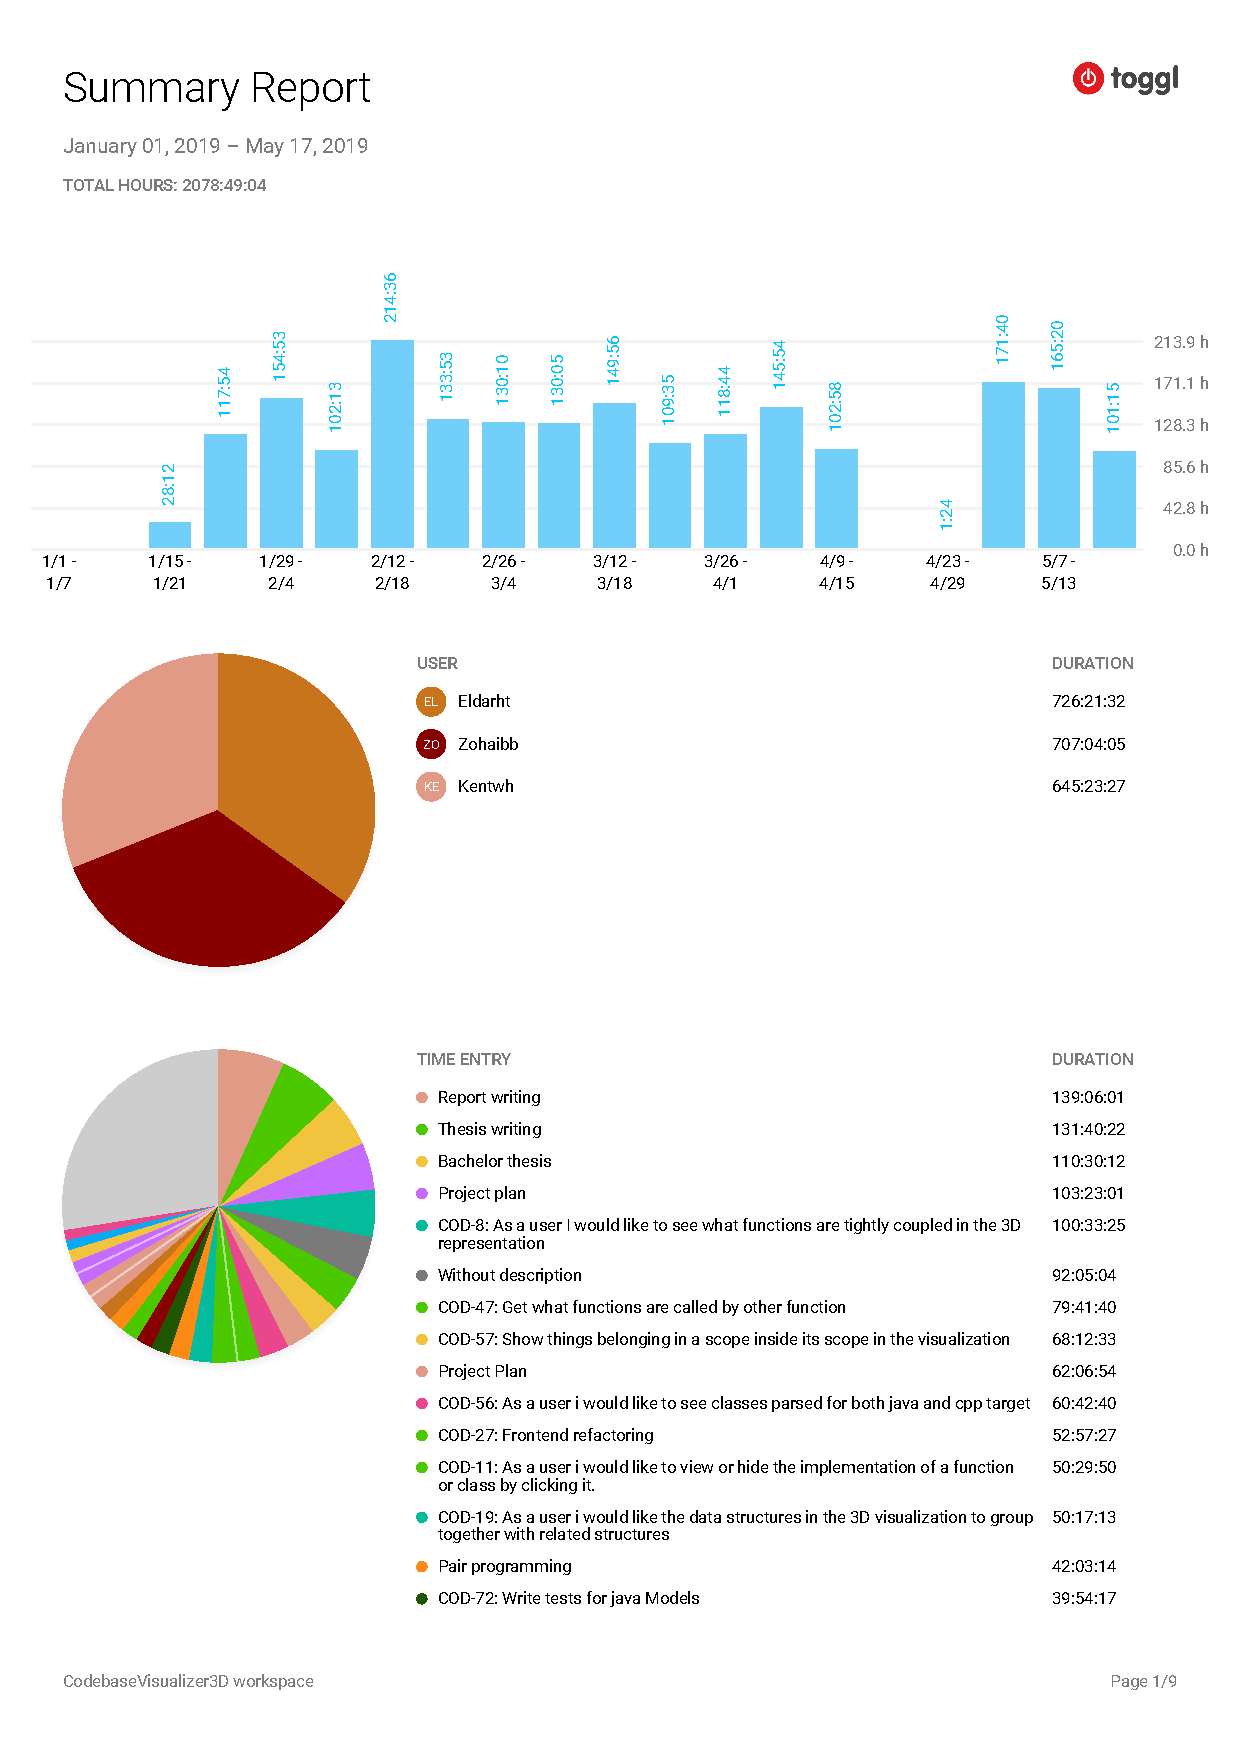
\includepdf[pages={-}]{inc/generalAppendix/togglSummary.pdf}
%\input{inc/worklog}

\end{document}
